\documentclass[10pt]{article}
\usepackage[hmargin=20mm,vmargin=20mm]{geometry}
\usepackage{amsmath, amsthm, amssymb, mathabx, verbatim, setspace, enumerate,mathtools}
\usepackage{relsize}
\usepackage[mathscr]{euscript}
\usepackage[all,cmtip]{xy}
\usepackage{relsize}
\usepackage[toc,page]{appendix}
\usepackage{arydshln}


\usepackage{tikz-cd}
\usetikzlibrary{patterns}


\xyoption{rotate}
\xyoption{pdf}


\usepackage{tikz-cd}


\linespread{1.1}

%prevents underfill for URLs in references
\usepackage{url}
\Urlmuskip=0mu plus 1mu\relax

%hyperlinked ToC
\usepackage{hyperref}



\newtheorem{thm}{Theorem}[section]
\newtheorem{prop}[thm]{Proposition}
\newtheorem{lemma}[thm]{Lemma}
\newtheorem{cor}[thm]{Corollary}

\theoremstyle{definition}
\newtheorem{exmp}[thm]{Example}
\newtheorem{defn}[thm]{Definition}
\newtheorem{rmk}[thm]{Remark}
\newtheorem{notation}[thm]{Notation}
\newtheorem{exercise}[thm]{Exercise}
\newtheorem{question}[thm]{Question}

\DeclareMathOperator{\Stab}{Stab}
\DeclareMathOperator{\Hom}{Hom}
\newcommand{\colim}{\operatornamewithlimits{colim}}
\DeclareMathOperator{\Sh}{Sh}
\DeclareMathOperator{\Pro}{Pro}
\DeclareMathOperator{\Ind}{Ind}
\DeclareMathOperator{\Ext}{Ext}
\DeclareMathOperator{\ch}{ch}
\DeclareMathOperator{\supp}{supp}
\DeclareMathOperator{\Coh}{Coh}
\DeclareMathOperator{\dmod}{-mod}
\DeclareMathOperator{\dperf}{-perf}
\DeclareMathOperator{\dcmod}{-cmod}
\DeclareMathOperator{\Spec}{Spec}
\DeclareMathOperator{\im}{im}
\DeclareMathOperator{\gr}{gr}
\DeclareMathOperator{\Td}{Td}
\DeclareMathOperator{\at}{at}
\DeclareMathOperator{\Sym}{Sym}
\DeclareMathOperator{\shHom}{\mathcal{H}\emph{om}}
\DeclareMathOperator{\shExt}{\mathcal{E}\emph{xt}}
\DeclareMathOperator{\Mod}{Mod}
\DeclareMathOperator{\DMod}{DMod}
\DeclareMathOperator{\pt}{pt}
\DeclareMathOperator{\defect}{def}
\DeclareMathOperator{\codim}{codim}
\DeclareMathOperator{\coker}{coker}
\DeclareMathOperator{\dR}{dR}
\DeclareMathOperator{\grr}{gr}
\DeclareMathOperator{\Hilb}{Hilb}
\DeclareMathOperator{\Quot}{Quot}
\DeclareMathOperator{\opp}{op}
\DeclareMathOperator{\Aff}{Aff}
\DeclareMathOperator{\Tor}{Tor}
\DeclareMathOperator{\Der}{Der}
\DeclareMathOperator{\End}{End}
\DeclareMathOperator{\Res}{Res}
\DeclareMathOperator{\QCoh}{QCoh}
\DeclareMathOperator{\tr}{tr}
\DeclareMathOperator{\DCoh}{DCoh}
\DeclareMathOperator{\Perf}{Perf}
\DeclareMathOperator{\Frac}{Frac}
\DeclareMathOperator{\IndCoh}{IndCoh}
\DeclareMathOperator{\Ho}{Ho}
\DeclareMathOperator{\Proj}{Proj}
\DeclareMathOperator{\Rep}{Rep}
\DeclareMathOperator{\cone}{cone}
\newcommand{\AAA}{\mathbb{A}}
\DeclareMathOperator{\Tot}{Tot}
\DeclareMathOperator{\ICoh}{ICoh}
\DeclareMathOperator{\Gal}{Gal}
\DeclareMathOperator{\Tate}{Tate}
\DeclareMathOperator{\rk}{rk}
\DeclareMathOperator{\Pic}{Pic}
\DeclareMathOperator{\Map}{Map}
\DeclareMathOperator{\Fun}{Fun}
\DeclareMathOperator{\LMod}{LMod}


%Complicated commands
\newcommand{\leftexp}[2]{{\vphantom{#2}}^{#1}{#2}}

%Sheafy commands
\newcommand{\sEnd}{\mathcal{E}\emph{nd}}


%Shorthand commands
\newcommand{\dd}{\partial}
\newcommand{\ra}{\rightarrow}
\newcommand{\la}{\leftarrow}
\newcommand{\mf}{\mathfrak}
\newcommand{\bs}{\backslash}
\newcommand{\cat}{\mathbf}
\newcommand{\wh}{\widehat}
\newcommand{\mc}{\mathcal}
%mathbb
\newcommand{\PP}{\mathbb{P}}
\newcommand{\Z}{\mathbb{Z}}
\DeclareMathOperator{\Gr}{Gr}
\DeclareMathOperator{\kchar}{char}
\newcommand{\C}{\mathbb{C}}
\newcommand{\R}{\mathbb{R}}
\newcommand{\N}{\mathbb{N}}
\DeclareMathOperator{\Ann}{Ann}
\newcommand{\A}{\mathbb{A}}
\newcommand{\G}{\mathbb{G}}
\newcommand{\Q}{\mathbb{Q}}
%mathcal
\newcommand{\OO}{\mathcal{O}}
\newcommand{\DD}{\mathcal{D}}
\newcommand{\LL}{\mathcal{L}}
\newcommand{\LLf}{\widehat{\LL}}
%mathfrak
\newcommand{\h}{\mf{h}}
\newcommand{\g}{\mf{g}}


\DeclareMathOperator{\Aut}{Aut}
%Typo correction
\newcommand{\tidle}{\tilde}
\newcommand{\rightarrw}{\rightarrow}
\newcommand{\alhpa}{\alpha}
\newcommand{\rigtarrow}{\rightarrow}
\newcommand{\emoh}{\emph}
\newcommand{\codts}{\cdots}
\newcommand{\shEnd}{\sEnd}
\newcommand{\rihgtarrow}{\rightarrow}


%Markup
\newcommand{\todo}[1]{\textbf{\textcolor{red}{TODO #1}}}

\newcommand{\loccit}{\emph{loc. cit. }} 

\setcounter{tocdepth}{2}


\title{Algebraic Geometry II notes}
\author{Harrison Chen}


\begin{document}
\maketitle
\tableofcontents

\newpage




\section{Differentials}

\subsection{Affine (algebraic) definition}


We will give three definitions of differentials.

\begin{defn}[Algebraic definition]
We will give the definition when $X = \Spec(R)$ and $S = \Spec(k)$ are affine, and leave it to the reader to glue.  We define $\Omega^1_{X/S}$ to be the free $R$-module with basis $\{dx \mid x \in R\}$ modulo the relations $ds = 0$ for $s \in k$, $d(x+y)=dx + dy$ and $d(xy) = xdy + ydx$ for $x,y\in R$.  We define the universal derivation by
$$d: \OO_X \rightarrow \Omega^1_X \;\;\;\;\;\; x \mapsto dx.$$
Note that $d$ is only $k$-linear, not $R$-linear.
\end{defn}

\begin{exmp}
Here are some of the basic examples to work out
\begin{enumerate}
\item $X = \mathbb{A}^n$; for $n=1$, it may be worthwhile to work out what the universal derivation $d$ is explicitly using the power rule,
\item if $k \rightarrow R$ is surjective, then $\Omega^1_{R/k} = 0$, 
\item if $k \rightarrow R$ is a localization, then $\Omega^1_{R/k} = 0$
\item if $R = k[x, y]/y^2 - x(x+1)(x-1)$, i.e. a smooth elliptic curve, check that $\Omega^1_{R/k}$ is a line bundle (it is only a locally free module, so you will have to remove points; interpret the differentials $dx$ and $dy$ on each open)
\item if $R = k[x,y]/y^2 - x^3$, i.e. a cuspidal curve, show it is not locally free.
\end{enumerate}
\end{exmp}

\begin{defn}[Pullback of differentials]
Given a commutative square
$$\begin{tikzcd}
X' \arrow[r, "f"] \arrow[d] & X \arrow[d] \\
S' \arrow[r] & S
\end{tikzcd}$$
we have a natural map $f^* \Omega^1_{X/S} \rightarrow \Omega^1_{X'/S'}$ defined by $dx \mapsto d(f^*x)$.  If the square is Cartesian then the map is an isomorphism.
\end{defn}


\begin{rmk}
Of particular interest is the case when $S' = S$, i.e.
$$\begin{tikzcd}
X \arrow[r, "f"] \arrow[d] & Y \arrow[d] \\
S \arrow[r] & S
\end{tikzcd}$$
where we obtain a natural pullback of $S$-relative forms $f^* \Omega^1_{Y/S} \rightarrow \Omega_{X/S}$.  Also of interest is the case $X'=X$, i.e.
$$\begin{tikzcd}
X \arrow[r, "f"] \arrow[d] & X \arrow[d] \\
Y \arrow[r] & S
\end{tikzcd}$$
where we obtain a natural ``quotient by vertical forms along $f$'' map $\Omega^1_{X/S} \rightarrow \Omega^1_{X/Y}$.  These two assemble into a sequence
$$f^* \Omega^1_{Y/S} \rightarrow \Omega^1_{X/S} \rightarrow \Omega^1_{X/Y}$$
\end{rmk}




\begin{prop}
Let $X \rightarrow Y$ be a map of $S$-schemes.  The sequence
$$f^* \Omega^1_{Y/S} \rightarrow \Omega^1_{X/S} \rightarrow \Omega^1_{X/Y}$$
is right exact.%  If the Jacobian (see below) for $f: X \rightarrow Y$ has nonvanishing maximal minor, then it is left exact.
\end{prop}
\begin{proof}
Left as exercise in the affine case.  Later we will define the sheaf of differentials in the non-affine case, and the claim will follow from the affine calculation.
\end{proof}


\begin{rmk}
The intuition here is that cotangent vectors relative $f: X \rightarrow Y$ are the quotient by those pulled back from $Y$, i.e. the ``vertical'' ones.  This is dual to the intuition for tangent vectors, where the relative tangent vectors are those which vanish under pushforward.
\end{rmk}

\begin{exmp}[Not left exact]
If we take $X = S = \pt$, then the sequence will not be left-exact in general.
\end{exmp}



\begin{exmp}
If $R = k[x_1, \ldots, x_n]/(f_1, \ldots, f_r)$, then we define the (dual\footnote{This is the transpose of the usual Jacobian matrix from multivariable calculus, since that matrix is used to push forward tangents whereas ours is the pullback on cotangents.}) \emph{Jacobian matrix} to be
$$J_f = \begin{pmatrix} \frac{df_1}{dx_1} & \cdots & \frac{df_r}{dx_1} \\ 
\vdots & \ddots & \vdots \\
\vdots & \ddots & \vdots \\
 \frac{df_1}{dx_n} & \cdots & \frac{df_r}{dx_n} \end{pmatrix}$$
Let $Q = k[x_1, \ldots, x_n]$ and $I = (f_1, \ldots, f_r)$ so that $R = Q/I$.  The Jacobian is a matrix $J: Q^{\oplus r} \rightarrow Q^{\oplus n}$, and is a realization of the pullback map along the map $f: \mathbb{A}^n \rightarrow \mathbb{A}^r$ defined by $f = (f_1, \ldots, f_r)$, i.e.
$$J_f: f^* \Omega^1_{\mathbb{A}^r_k/k} \rightarrow \Omega^1_{\mathbb{A}^n_k/k}$$
By right exactness of the relative differentials sequence, we have that $\coker(J_f) \simeq \Omega^1_{\mathbb{A}^n_k/\mathbb{A}^r_k}$.  In particular, since we have a Cartesian square
$$\begin{tikzcd}
X \arrow[r, "i"] \arrow[d] & \mathbb{A}^n_k \arrow[d, "f"] \\
\Spec(k) \arrow[r, "0"] & \mathbb{A}^r_k
\end{tikzcd}$$
we find that $i^*\coker(J_f) = \coker(i^* J_f) \simeq \Omega^1_{X/k}$.  Practically speaking, what this tells us is that $\Omega^1_{X/k}$ is the $R$-module generated by the $dx_i$ modulo the relations $d(f_j)$.
%In fact this is a more general fact.  \todo{functoriality map, and also when is it an iso?}  i.e. $\Omega^1_{\mathbb{A}^n_S/\mathbb{A}^r_S} \simeq \Omega^1_{X/S}$.  This is a Cartesian diagram, and the LHS is comptued by the usual exact sequence (only get cokernel!)
\end{exmp}



\begin{exmp}
Although we won't discuss how to glue, let us do an example of how to do it in practice.  Let $X = \mathbb{P}^1_k$.  Cover $X$ with affine opens $U_0 = \Spec k[x]$ and $U_\infty = \Spec k[y]$, where $xy = 1$ on the intersection $U_{0\infty}$.  Then, we have (noting that $d(xy - 1) = x\;dy + y\;dx$):
$$\Omega^1_{U_0} = k[x] \; dx, \;\;\;\;\;\;\; \Omega^1_{U_\infty} = k[y] \; dy, \;\;\;\;\;\;\; \Omega^1_{0\infty} = \frac{k[x,y]}{xy-1} \; dx, dy / \langle x\; dy + y \;dx \rangle.$$
In particular, the gluing relation on the intersections is $dy = -x^{-2} \; dx$, so $\Omega^1_{\mathbb{P}^1_k} \simeq \OO_{\mathbb{P}^1_k}(-2)$.
\end{exmp}



\begin{prop}
If $R$ is a finitely generated (resp. presented) $k$-algebra, then $\Omega^1_{R/k}$ is a finitely generated (resp. presented) $R$-module.
\end{prop}
\begin{proof}
The argument for finitely presented is essential our discussion of the Jacobian above.  For finite generation, we can replace $\mathbb{A}^r_k$ with $\prod \mathbb{A}^1_k$.
\end{proof}



\begin{defn}
Let $X$ be a scheme and $i: Z \subset X$ a closed subscheme with ideal sheaf $\mathcal{I}$.  We define the \emph{conormal bundle} $\mathcal{N}^\vee_{Z/X}$ of $Z$ to be $\mathcal{I}/\mathcal{I}^2 = i^* \mathcal{I}$.
\end{defn}

\begin{rmk}
Let's motivate this.  Recall that in calculus, a power series at $0 \in \mathbb{A}^1$ is given by
$$a_0 + a_1 t + \frac{a_2}{2!} x^2 + \frac{a_3}{3!} + \cdots \in \lim_n k[x]/x^n$$
and in particular, if $R = k[x]$ and $I = (x)$ is the ideal sheaf, lives in $\lim_n R/I^n$.  

Given a function $f$, its Taylor series is such a power series.  However, in order to be coordinate independent, one should really write
$$f(0) + \frac{df}{dx}(0) \, dx + \frac{1}{2!}\frac{d^2f}{dx}(0) \, (dx)^2 + \cdots$$
and in particular, the first order term comprises of the normal covectors to $Z \subset X$, and corresponds to $I/I^2 \subset R/I^2$ in the infinitesimal neighborhood.
\end{rmk}

The proof of the following in the affine case is left as an exercise.
\begin{thm}
Let $Z \hookrightarrow X$ be a closed immersion.  There is an exact sequence
$$i^* \mathcal{N}^\vee_{Z/X} \rightarrow \Omega^1_{X/S} \rightarrow \Omega^1_{Z/Y} \rightarrow 0$$
\end{thm}

\begin{rmk}
Proving this theorem can also serve as motivation for the definition of conormal bundle.  The normal bundle to a submanifold $Z \subset X$ consists of the tangents in $X$ modulo tangents pushed forward from $Z$.  It really is a quotient and not a sub, because in the absence of an inner product on tangents there is no way to say what it means to be perpendicular.  The above sequence can be thought of as the dual to the corresponding sequence for tangents.
\end{rmk}

\begin{exmp}
This does not have to be exact.  For example, if $Z = \Spec k[x]/x^2$ and $X = \Spec k[x]$, then $I/I^2 = (x^2)/(x^4)$ where $x^3 \mapsto 3x^2 \; dx = 0$.
\end{exmp}



\subsection{Local complete intersections} 


\begin{prop}
Let $X$ be a Noetherian scheme, and $Z \hookrightarrow X$ a local complete intersection of codimension $r$.  Then, $\mathcal{N}^\vee_{Z/X}$ is locally free of rank $r$.

Locally, if $X = \Spec(R)$ and $Z = \Spec(R/I)$ where $I = (f_1, \ldots, f_r)$ is generated by a regular sequence (i.e. is a complete intersection), then $I/I^2$ is free with basis $f_1, \ldots, f_r$.
\end{prop}


We will use the following theorem in an essential way.  Recall that a sequence $f_1, \ldots, f_r \in R$ is \emph{regular} if $f_k$ is a non-zerodivisor in $R/(f_1, \ldots, f_{k-1})$.
\begin{thm}
Let $(A, \mf{m})$ be a Noetherian local ring.  Any permutation of a regular sequence of elements in $\mf{m}$ is regular.
\end{thm}
\begin{proof}
It suffices to consider the case when $r=2$.  Consider the the total complex of the double complex
$$\begin{tikzcd}
R \arrow[r, "x"] & R \\
R \arrow[r, "x"] \arrow[u, "y"] & R \arrow[u, "y"]
\end{tikzcd}$$
Denote the chain complex by $C$.  We claim that $H^{-1} = H^{-2} = 0$ if and only if $x, y$ is a regular sequence.    The backwards direction we will leave as an exercise.  For the forward direction, note that $\Ann(x) \oplus 0 \subset Z^{-1}$.  The restriction of the map $d: C^{-2} \rightarrow C^{-1}$ induces a map $\Ann(x) \rightarrow \Ann(x) \oplus 0$, which is surjective since $H^{-1} = 0$.  By Nakayama, since $y \in \mf{m}$, we have that $\mf{m}\Ann(x) = \Ann(x)$, i.e. $\Ann(x) = 0$.  Thus, $x$ is a non-zerodivisor.

Next, suppose $(a, b) \in Z^{-1}$, i.e. $xa = yb$.  It must be killed by a coboundary, say $c \in C^{-2}$ so that $yc = a$ and $xc = b$.  Taking everything modulo $x$, this means that if $yb \equiv 0 \pmod{x}$ then $b \equiv 0 \pmod{x}$, i.e. $y$ is a non zerodivisor modulo $x$.
\end{proof}

We now prove the result.
\begin{proof}
First, note that regular sequences are preserved under localization (i.e. if $f$ is a non-zerodivisor in $R$, then $f$ is a non-zerodivisor in $S^{-1}R$).  Next, note that $S^{-1}I/S^{-1}I^2 = S^{-1}(I/I^2)$, as localization is exact.  We've reduced to the case when $R$ is a local ring.

Now, suppose $\sum a_i f_i = 0$ for $a_i \in R$.  Since $f_r$ is a non-zerodivisor in $R/(f_1, \ldots, f_{r-1})$, then $a_r f_r \equiv 0 \pmod{f_1, \ldots, f_{r-1}}$ implies that $a_r \equiv 0 \pmod{f_1, \ldots, f_{r-1}}$.  In particular, $a_r \in I$.  Permuting the sequence, find that all $a_i \in I$, so $\sum a_i f_i \in I^2$.  Thus, the map $R/I^{\oplus r} \rightarrow I/I^2$ taking  $(a_1, \ldots, a_r) \mapsto \sum a_i f_i$ is injective.  It is surjective by construction.
\end{proof}


\subsection{Definition by universal property}

\begin{defn}[Differentials by universal property]
Let $X$ be a scheme over $S$.  Let $\mathcal{M}$ be a quasicoherent sheaf on $X$.  An $S$-linear $\mathcal{M}$-valued \emph{derivation} is an $f^{-1}\OO_S$-linear map $D: \OO_X \rightarrow \mathcal{M}$ such that $D(xy) = xD(y) + D(x)y$.  Denote by $\Der_{X/S}(\mathcal{M})$ the sheaf of $\OO_S$-modules of $S$-linear $\mathcal{M}$-valued derivations on $X$.

We define $\Omega^1_{X/S}$ to be the quasicoherent sheaf on $X$ representing the functor $\Der_{X/S}$.  Equivalently, such that $\Hom_X(\Omega^1_{X/S}, \mathcal{M}) = \Der_{X/S}(\mathcal{M})$.  Equivalently, such that for any derivation $D$ as above, there is a natural factorization
$$\begin{tikzcd}
\OO_X \arrow[dr, "d"] \arrow[rr, "D"] & & \mathcal{M} \\
& \Omega^1_{X/S} \arrow[ur, dotted] &
\end{tikzcd}$$
\end{defn}

\begin{rmk}
The sheaf of ($\OO_X$-valued) derivations is an algebraic analogue of the sheaf of vector fields on $X$.  The universal vector field on $\Omega^1_{X/S}$ is, in local coordinates $x_1, \ldots, x_n$, given by $f \mapsto \sum \frac{d}{dx_i} \; dx_i$.
\end{rmk}

\begin{prop}
This definition is equivalent to the algebraic definition.
\end{prop}
\begin{proof}
We will prove this for affines; the global result follows by taking an open affine cover.  On affines, simply define the dotted arrow by $dx \mapsto D(x)$.  We leave as an exercise that such a map is well-defined.
\end{proof}

\subsection{Global definition by conormals}

We now arrive at our third definition.   The intuition comes from complex geometry, i.e. if $X$ is a complex manifold, then $\Omega^1_{X \times X} = \Omega^1_X \oplus \Omega^1_X$, and the restriction to the diagonal takes $(\omega_1, \omega_2) \mapsto \omega_1 + \omega_2$.  Then, the conormal is isomorphic to $\Omega^1_X$ realized as a (split) submodule given by $(\omega, -\omega)$.  \emph{Note the choice of sign in choosing an isomorphism.}

This definition will seem deceptively elegant; it will take a bit more work to define the universal derivation than before.
\begin{defn}[Differentials by conormal bundles]
Let $\mathcal{I}_\Delta$ denote the ideal sheaf\footnote{We do not assume that $X$ is separated.  The diagonal is always locally closed, and the definition of ideal sheaf still makes sense by gluing over an open affine cover.} of the diagonal $\Delta: X \rightarrow X \times_S X$ (which is always locally closed).  We define
$$\Omega^1_{X/S} := \mathcal{I}_\Delta/\mathcal{I}_\Delta^2.$$
\end{defn}

\begin{defn}[Principal parts and universal derivation]
Let $\mathcal{P}^1_{X/S}$ denote the \emph{sheaf of principal parts to first order}, which we define to be:
$$\mathcal{P}^1_{X/S} := \Delta^{-1} \OO_{X \times_S X}/\mathcal{I}^2_{\Delta}.$$
A priori, this is just a sheaf on $X$, not a sheaf of $\OO_X$-modules.  There are two $\OO_X$-module structures on $\mathcal{P}^1_{X/S}$, coming from the $\pi_i^{-1}\OO_X$-module structures on $\OO_{X \times_S X}$ for $i=1,2$ (where $\pi_i$ are the projections) and the identity $\Delta^{-1} \pi_i^{-1} \OO_X = \OO_X$.  \emph{We declare, once and for all, that we take the $\OO_X$-module structure by taking $i=1$.  Taking $i=2$ would amount to a sign change.}

We define the universal derivation $d: \OO_X \rightarrow \Omega^1_X$ to be $\pi_2^* - \pi_1^*: \OO_X \rightarrow \mathcal{P}^1_{X/S}$ where $\pi_i^*$ is given by the action of $f \in \OO_X$ on $1 \in \Delta^{-1}\OO_{X \times_S X}$ under the corresponding $\OO_X$-module structure.  Note that $d$ always lands in $\Delta^{-1} \mathcal{I}_\Delta \subset \Delta^{-1} \OO_{X \times_S X}$, so this makes sense.
\end{defn}

\begin{rmk}
Equivalently, we can identify
$$\mathcal{P}^1_{X/S} := \pi_{i,*}(\OO_{X \times_S X}/\mathcal{I}^2_{\Delta})$$
which gives two different $\OO_X$-module structures for $i=1,2$.  
\end{rmk}

\begin{rmk}[Principal parts exact sequence]
By definition, there is a short exact sequence (the extension of principal parts):
$$0 \rightarrow \Omega^1_{X/S} \rightarrow \mathcal{P}^1_{X/S} \rightarrow \OO_{X/S} \rightarrow 0.$$
This defines the \emph{Atiyah class} $\mathrm{at}_X \in H^1(X, \Omega^1_{X/S})$ when $X \rightarrow S$ is smooth (otherwise, it is not the right notion, though it is well-defined).
\end{rmk}

\begin{exmp}
Let us unwind this definition in the case $S = \Spec k$ for $k$ a field, and $X = \mathbb{A}^1_k = \Spec k[x]$.  We will use the notation $x_1 := x \otimes 1$ and $x_2 := 1 \otimes x$.  Then, $P^1_{X/S} = k[x_1, x_2]/(x_2 - x_1)^2$ and $\Omega^1_{X/S} = (x_2 - x_1)/(x_2-x_1)^2$.  The universal derivation takes
$$x \mapsto x_2 - x_1$$
$$x^2 \mapsto x_2^2 - x_1^2 \equiv 2x_2(x_2-x_1) \equiv -2x_1(x_2 - x_1)$$
We leave the computation of $d(x^n)$ as an exercise.  Note the dependence of choice: if we let $\OO_X$ act through $\pi_2$ instead, we get a difference in sign.
\end{exmp}

\begin{prop}
The global definition is equivalent to the algebraic definition on affines.
\end{prop}
\begin{proof}
We define a map $\Omega^1_{X/S} \rightarrow I_\Delta/I^2_\Delta$ by sending $dx \mapsto 1 \otimes x - x \otimes 1$.  It is clearly additive and $k$-linear.  It satisfies the Leibniz rule since
$$d(xy) \mapsto 1 \otimes xy - xy \otimes 1$$
$$x d(y) + y d(x) \mapsto x \otimes y - xy \otimes 1 + y \otimes x - xy \otimes 1$$
and the difference is
$$(1 \otimes x - x \otimes 1)(1 \otimes y - y \otimes 1) = 1 \otimes xy + xy \otimes 1 - x \otimes y - y \otimes x.$$

To see that it is surjective, we claim that $I$ is generated by elements of the form $1 \otimes x - x \otimes 1$.  Suppose that we have $\sum x_i \otimes y_i$ such that $\sum x_i y_i = 0$.  Then, $\sum x_i \otimes y_i = \sum x_i \otimes y_i - x_i y_i \otimes 1 = (x_i \otimes 1) \sum 1 \otimes y_i - y_i \otimes 1$.

To see that it is injective, we define a left inverse by $x \otimes y \mapsto x \; dy$.  It is clearly a left inverse, but we need to check it is well-defined.  To this end, we need to show that the following expression maps to zero
$$(\sum x_i \otimes y_i)(\sum x_j' \otimes y_j') = \sum x_j x_j' \otimes y_j y_j'$$
where $\sum x_i y_j = \sum x_j' y_j' = 0$.  The image of the expression is
$$\sum x_i x_j d(y_i y'_j) = \sum x_i x_j' y_i d(y_j') + x_i x_j' y_j' d(y_i)$$
$$(\sum x_i y_i)(\sum y_i d(y_j') + (\sum x_i d(y_i))(\sum y_i y_j') = 0.$$
\end{proof}


\newpage

\section{Smoothness and differentials}

\subsection{Review of dimension}

Let us recall some definitions and results from the first semester.  
\begin{defn}
The \emph{dimension} of a scheme $X$, which we denote $\dim(X)$, is the maximum length of a chain of irreducible closed subsets.  Affine locally, coincides with \emph{Krull dimension}: maximal length of chain of prime ideals (which correpsond to irreducible closed subsets).  We say $X$ is \emph{pure dimension} $d$ if all of its irreducible components have dimension $d$.  A local ring $(A, \mf{m})$ is \emph{regular} if it is Noetherian and the minimal number of generators of $\mf{m}$ is equal to its Krull dimension, and we say $X$ is \emph{regular} if its local rings are regular.

Let $X$ be a scheme and $Y \subset X$ an irreducible subset.  The \emph{codimension} of $Y$ is the maximum length of irreducible closed subsets containing $Y$.  Affine locally, this coincides with the notion of \emph{height} of a prime ideal (corresponding to the generic point of the closure of $Y$), which is also the dimension of $R_{\mf{p}}$.
\end{defn}

We won't prove this.  It's Vakil Theorem 11.2.9
\begin{thm}
Let $X$ be a pure-dimensional locally of finite type $k$-scheme.  For any irreducible subset $Y$, we have $\codim_X(Y) + \dim(Y) = \dim(X)$.
\end{thm}

%\begin{exmp}
%The theorem can fail for somewhat silly reasons.  For example, take $X = \mathbb{A}^1 \coprod \mathbb{A}^3$, and take $x \in \mathbb{A}^1$.  Then $\codim_X(x) = 1$, $\dim(x) = 0$ and $\dim(X) = 3$.
%
%It can also fail for less silly reasons, essentially because localization (which produces non finite type schemes) does not ``commute'' with the notion of codimension.  Take $k[x, t]$ and consider $V(xt - 1)$.  It is dimension 1, codimension 1, which adds up to 2, which is fine.
%
%Now, let's take $k[x]_{(x)}[t]$ and consider the same variety.  The problem ehre is that $V(xt-1)$ has dimension 0, \todo{fiinish}
%\end{exmp}

See Theorems 11.3.2 and 11.3.7 in Vakil.
\begin{thm}[Krull principal ideal theorem, Krull height theorem]
Let $X$ be a locally Noetherian scheme, and $f \in \OO(X)$.  The irreducible components of $V(f)$ have codimension 0 or 1.  More generally, if $f_1, \ldots, f_r \in \OO(X)$, then the irreducible components of $V(f_1, \ldots, f_r)$ have codimension at most $r$.
\end{thm}

\begin{thm}
Let $(A, \mf{m})$ be a local ring.  Then $\dim(A) \leq \dim_k(\mf{m}/\mf{m}^2)$.
\end{thm}
\begin{proof}
Follows from Nakayama and Krull's height theorem.
\end{proof}



\subsection{Smoothness over a field}


\begin{prop}[Jacobian criterion for regularity]
Let $k$ be an algebraically closed field, $X$ a finite type $k$-scheme of pure dimension $d$, and $x \in X$ a $k$-point.  Choose an open affine neighborhood $U$ of $x$ such that $U = k[x_1, \ldots, x_n]/(f_1, \ldots, f_r)$.  Then $X$ is regular at $x$ if and only if the cokernel of the Jacobian $J$ at $x$ has dimension $d$.
\end{prop}
\begin{proof}
Since the question is entirely local, we can take $X = U$, i.e. $X = \{0\} \times_{\mathbb{A}^r_{k}} \mathbb{A}^n_{k}$.  We will define a sequence of Jacobians.  First, we have
$$J_{\mathbb{A}^n_k}: \OO_{\mathbb{A}^r_k}^{\oplus r} \rightarrow  \OO_{\mathbb{A}^r_k}^{\oplus n} $$
whose cokernel is $\Omega^1_{\mathbb{A}^n_k/\mathbb{A}^r_k}$.  Its pullback to $X$ is $\Omega^1_{X/k}$, and by right-exactness of tensor products it induces
$$J_X: \OO_{X}^{\oplus r} \rightarrow \OO_{X}^{\oplus n}$$
whose cokernel is $\Omega^1_{X/k}$.  Since localization is exact, we also have
$$J_{X, x}: \OO_{X,x}^{\oplus r} \rightarrow \OO_{X,x}^{\oplus n}$$
whose cokernel is $\Omega^1_{X/k, x}$.
Specializing at the residue fields, we have a map of vector spaces
$$J_{\kappa(x)}: \kappa(x)^r \rightarrow \kappa(x)^n$$
whose cokernel is $\Omega^1_{X/k, x} \otimes_{\OO_{X, x}} \kappa(x) = \mf{m}/\mf{m}^2$.  By Nakayama, the number of minimal generators is equal to the dimension of $\mf{m}/\mf{m}^2$, so the result follows.  Note that we need $k$ to be algebraically closed so that $\kappa(x) = k$, to apply Hartshorne Proposition II.8.7 (i.e. that the fiber of the sheaf of differentials is isomorphic to the cotangent space requires that $\kappa(x) = k$).
\end{proof}

%\begin{rmk}
%\todo{WTFFF}
%Vakil 21.2.18: fiber of $\Omega$ at $k$-point is cotangent space (no need for alg closed)
%Vakil 21.3.9: extends to $\kappa(x)$ separable over $k$
%21.1.G: Exercise that shows that Jacobian cuts out Zariski cotangent space at $k$-points \todo{MORE GENERAL???}  Yes: works for separable points too
%21.3.9 "important corollary"
%\end{rmk}



\begin{defn}[Smoothness over a field $k$]
Let $X$ be a $k$-scheme.  We say $X$ is \emph{smooth of dimension $d$} over $k$  if it is pure of dimension $d$, and if there is an open affine cover by schemes of the form $\Spec(k[x_1, \ldots, x_r]/(f_1, \ldots, f_r))$ such that the Jacobian has corank $d$ at all (possibly non-closed) points.
\end{defn}

\begin{rmk}
Under this definition, $\R[x]$ is smooth even though it has cotangent spaces of dimension greater than its dimension.  So, the Jacobian criterion is somehow ``smarter'' than the cotangent space when $k$ is not algebraically closed.
\end{rmk}

%\todo{is the following really correct??  i guess its nota sserting nonempty, or dense}
\begin{prop}
It suffices to check the above condition on closed points.
\end{prop}
\begin{proof}
Recall that a matrix has rank $r$ if there is an $r \times r$ minor which does not vanish and if all $(r+1) \times (r+1)$ minors vanish.  The former is an open condition (i.e. a union of opens) and the latter is a closed condition (i.e. intersection of closed).  The latter condition, however, is automatic -- the Jacobian can never have rank greater than $d$ at any point since $\dim(\mf{m}/\mf{m}^2) = n - \text{rank}(J)$ cannot exceed the Krull dimension $d$, so smoothness is an open condition.  The only open set containing all closed points is $X$ itself.
\end{proof}


\begin{thm}[Regular vs. smooth]
Let $k$ be a field.  Every smooth $k$-scheme is regular.  If $k$ is perfect, then every regular finite-type $k$-scheme is smooth.% \todo{why finite type...}
\end{thm}
%\begin{proof}
%\todo{insert} proof postponed???
%\end{proof}

\begin{rmk}
Note that an algebraically closed field is always perfect, so our Jacobian criterion is a special case of the above.
\end{rmk}

\begin{exmp}
The canonical example of a non-perfect field is $k = \mathbb{F}_p(t)$.  Take $X = \Spec k[x]/(x^p - t)$.  We have that $\OO(X)$ obtained by adjoining $p$th roots of $t$ to $k$, and is a field (i.e. $x^{-1} = x^{p-1}/t$).  On the other hand, the Jacobian condition fails since $\frac{d}{dx}(x^p - t) = 0$ (since $p = 0$).  Note that this is an example of a wildly ramified extension of $k$.
\end{exmp}


\begin{prop}
Let $X$ be a scheme over $k$ of finite type.  Then, $X$ is smooth over $k$ if and only if $\Omega^1_{X/k}$ is a locally free sheaf.  Furthermore, in this case, the $\dim(X) = \mathrm{rank}(\Omega^1_{X/k})$.
\end{prop}
%\begin{proof}
%We may assume that $X$ is affine, and moreover that $X = \Spec R$ where $R = k[x_1, \ldots, x_n]/(f_1, \ldots, f_r)$, and then furthermore replace $R$ with its localization at $0$.  Rearrange the equations and generators so that the ``upper left'' $(n-d) \times (n-d)$ minor has full rank.  There is a map $R^{\oplus d} \rightarrow \Omega^1_{X/k}$ sending $e_i \mapsto dx_{n-d+i}$.
%
%To see that the map is surjective, we can argue on cotangent spaces and use Nakayama.  To this end, there is an $r \times r$-matrix $E$ such that the upper left minor in $JE$ is the identity.    In particular, this expresses the $dx_j$ for $j \leq n-d$ in terms of the $dx_{n-d+i}$ for $i \geq 1$.
%
%To see that the map is injective, suppose we have $\sum a_i dx_{n-d+i} = 0$.
%
%\end{proof}



\subsection{Smoothness of a morphism}


We now seek to generalize the above to the case where $S$ is not a field.  The following definition is not the most elegant characterization of a smooth morphism, but it is the most direct and most in-line with intuition.
\begin{defn}
A map $f: X \rightarrow Y$ of schemes is \emph{smooth of relative dimension $d$} if there is an open cover $U_i$ of $X$ and a corresponding affine cover $V_i = \Spec(B_i)$ of $Y$ such that $U_i \subset f^{-1}(V_i)$, and further such that $U_i$ is an open subscheme of a scheme $W_i = \Spec(B_i[x_1, \ldots, x_{d+r}]/f_1, \ldots, f_r)$ such that there exists a maximal invertible minor of the corresponding Jacobian.
\end{defn}

\begin{exmp}
Under this definition, open immersions, and projections of the form $\mathbb{A}^n_S \times_S Y \rightarrow Y$ are smooth.  More generally, projections of the form $X \times_S Y \rightarrow Y$ are smooth where $X$ is affine over $S$ and locally has vanishing Jacobian as described above.
\end{exmp}

\begin{rmk}
Let us motivate this definition.
\begin{enumerate}
\item First, we agree that that smoothness should be a local condition on both the source and target.  This means that $f: X \rightarrow Y$ is smooth if and only if for every $x \in X$ there is an open neighborhood $U$ and an open $V \subset Y$ with $U \subset f^{-1}(V)$ such that $f|_U$ is smooth.  This is the first part of the above definition.  (Note that in the definition we could have equivalently insisted that $U, V$ are affine.)
\item Second, we agree that open immersions should be smooth.  That way, if $W \rightarrow V$ is smooth, and $U \subset W$, then $U \rightarrow V$ should be smooth.
\item Next, for affine maps $W \rightarrow V$ we use the Jacobian condition above.  Note that the Jacobian condition here is stricter; we do not allow for ``too many equations'' and test only the maximal minors.
\end{enumerate}
\end{rmk}

\begin{rmk}
There is a possible alternative definition: we say $f: X \rightarrow Y$ is smooth if for every point $x \in X$ there is are affine opens $U \subset X$ and $V \subset Y$ such that $x \in U \subset f^{-1}(V)$, such that $U $??
\end{rmk}


Because of point (3) above, it is not clear that this notion is the same as our earlier notion over a field $k$.
\begin{thm}
Let $X$ be a $k$-scheme for $k$ a field.  Then $X$ is smooth of relative dimension $d$ over $\Spec(k)$ if and only if $X$ has pure dimension $d$ and is smooth over the field $k$.
\end{thm}
%\begin{proof}
%Let us prove the forward dimension, which amounts to showing that if $X$ is smooth of relative dimension $d$ over $\Spec(k)$, then $X$ is pure of dimension $d$.  Note that requiring that $X$ is pure of dimension $d$ was necessary for us to formulate the more relaxed Jacobian condition.  Since the question is Zariski local and open immersions do not change dimension, we can assume that $X = W$ as in the definition.
%
%First, let $X_{\bar{k}}$ denote the base change to the algebraic closure.  We note (and leave as an exercise) that $X$ is pure of dimension $n$ if (and only if) $X_{\bar{k}}$ is.  Since $W$ is cut out by $n+d$ equations in $n$ variables, it has dimension $\geq d$ (this is by repeatedly applying the Krull Principal Ideal Theorem, and carefully considering the definition of codimension).  On the other hand, by the Jacobian condition, the tangent spaces have dimension $d$, so $X$ has dimension $\leq d$.  %\todo{kind of sketchy}
%
%
%
%
%For the backwards direction, we need to show the following.  Suppose $X = \Spec k[x_1, \ldots, x_{m+d}]/(f_1, \ldots, f_r)$ has pure dimension $d$, and let $p \in X$ such that the cokernel of the Jacobian has dimension $d$.  There is a $m \times m)$ invertible minor; rearrange the generators and relations such that it is the ``upper left'' minor, and note that $r \geq m$.  We claim that there is an open $U$ such that the ideal $(f_1, \ldots, f_m)$ and $(f_1, \ldots, f_r)$ cut out the same locus away from $U$ (more precisely, $U$ is affine they are equal after localization).  Equivalently, we wish to show that $(f_{m+1}, \ldots, f_r) = 0$ after localization.  This is true on cotangent spaces by assumption, so by Nakayama 
%\end{proof}




Note that it is difficult to show that a morphism is not smooth using this definition.


\begin{prop}
Let $f: X \rightarrow S$ be a morphism of schemes, smooth of relative dimension $d$.  Then, $\Omega^1_{X/S}$ is locally free of rank $d$.
\end{prop}
%\begin{proof}
%Note that both conditions are affine local on $X$ and $S$, and also preserved by restricting along closed immersions.  Therefore, it suffices to consider the case 
%$$X = W = \Spec B[x_1, \ldots, x_{d+r}]/(f_1, \ldots, f_r) \rightarrow V = \Spec(B).$$
%In this case, note that $\Omega^1_{X/S} = \coker(J)$.  \todo{???}
%
%
%\todo{counterexample to converse?}
%\end{proof}



\begin{exmp}
The converse to the above is not true.  For example, take a closed embedding.  Alternatively, take $Y = \Spec k[x,y]/xy$ and $X$ to be its normalization.  The normalization is affine, $X = \Spec k[x,y]/y \times k[x,y]/x$.  Letting $R = k[x,y]/xy$, we have that $\OO(X) = R[s]/(s^2 - s, x(s-1), ys)$ (i.e. letting $s$ stand in for $(1, 0)$ and $1-s$ stand in for $(0, 1)$.  On one hand, the sheaf of relative Kahler differentials is zero, since $\Omega^1_{X/Y}$ is generated by $ds$ with relations $(2s-1)\, ds = 0$, $x \, ds = 0$, and $y\,ds=0$.  Multiplying the second relation by $s$ gives $s \, ds = 0$, and taking a linear combination with the first relation gives $ds = 0$.

On the other hand, the dimension of the two varieties is equal, but the Jacobian  is the matrix $\begin{pmatrix} 2s-1 & x & y\end{pmatrix}$ whose cokernel has dimension 1 at $s = \frac 1 2$, $x=y=0$.
\end{exmp}




\subsection{The cotangent complex}






We wish to prove the following theorem.
\begin{thm}
Let $X, Y$ be schemes over $S$.  Suppose that $f: X \rightarrow Y$ is smooth.  Then the relative differentials exact sequence is left exact:
$$0 \rightarrow f^* \Omega^1_{Y/S} \rightarrow \Omega^1_{X/S} \rightarrow \Omega^1_{X/Y} \rightarrow 0.$$
Suppose $i: Z \hookrightarrow X$ is a closed embedding.  If $Z$ is smooth over $k$, then the conormal exact sequence is left exact:
$$0 \rightarrow \mathcal{N}^\vee_{Z/X} \rightarrow i^* \Omega^1_{X/S} \rightarrow \Omega^1_{Z/S} \rightarrow 0.$$
\end{thm}
A subcase proof of the above can be found in Vakil.  Instead, I will introduce an axiomatic introduction to the \emph{cotangent complex} which gives this result more or less automatically.

%\begin{exmp}
%It may be worthwhile to illustrate the failure of exactness in two examples. 
%
%
%For the conormal exact sequence, note that if $Z$ is the nodal curve and $X$ is $\mathbb{A}^2$, then the first map will not be injective since the normal vector at $0$ ``does not know where to go.''  \todo{???}  On the other hand, if $Z$ is smooth, then 
%
%\end{exmp}


\begin{defn}
Let $X \rightarrow S$ be a map of schemes.  The cotangent complex $\mathbb{L}_{X/S}$ is an object of $D(\QCoh(X))^{\leq 0}$ satisfying the following properties.
\begin{enumerate}
\item given a commuting square
$$\begin{tikzcd}
X' \arrow[r, "f"] \arrow[d] & X \arrow[d] \\
S' \arrow[r] & S
\end{tikzcd}$$
there is a natural morphism $Lf^* \mathbb{L}_{X/S} \rightarrow \mathbb{L}_{X'/S'}$, which is an equivalence when the square is Cartesian,
\item for $f: X \rightarrow Y$ a morphism over $S$, there is an exact triangle
$$f^* \mathbb{L}_{Y/S} \rightarrow \mathbb{L}_{X/S} \rightarrow \mathbb{L}_{X/Y}$$
inducing the usual long exact sequence,
\item there is a natural homomorphism $\gamma: \mathbb{L}_{X/S} \rightarrow \Omega^1_{X/S}$ which induces an isomorphism on $H^0$ and which is an equivalence if $f$ is smooth,
\item if $f$ is a closed embedding, then there is a natural homomorphism $\beta: \mathbb{L}_{X/S} \rightarrow \mathcal{N}^\vee_{X/Y}[1]$ which induces an isomorphism on $H^{-1}$.
\end{enumerate}
\end{defn}

We can easily prove the above theorem using this machinery.
\begin{proof}
The relative differential exact sequence is simply the zeroth level of the long exact sequence.  To prove exactness on the left, it suffices to show that $H^1(\mathbb{L}_{X/Y}) = 0$, but this follows from smoothness of $f$.  The conormal exact sequence is left exact if $H^{-1}(\Omega^1_{Z/S}) = 0$, which also follows from smoothness.
\end{proof}

%
%Using these axioms, we can conclude the following.
%\begin{prop}
%If $Z$ is a local complete intersection in a smooth scheme $X$, then $H^i(\mathbb{L}_{Z/S})$ vanishes when $i \ne 0, 1$.  In particular, the conormal exact sequence is exact to the left.
%\end{prop}
%\begin{proof}
%We can check affine locally on both $X$ and $S$.  In particular, using the usual pullback diagram $X = \mathbb{A}^n_S \times_{\mathbb{A}^r_S} \{0\}_S$ and the exact triangle, we find that
%$$\mathbb{L}_{X/S} = \mathrm{cone}(i^* \mathbb{L}_{\mathbb{A}^r_S/S} \rightarrow  \mathbb{L}_{\mathbb{A}^n_S/S})$$
%which gives the desired result.
%\end{proof}
%
%\begin{prop}
%If $f: X \rightarrow Y$ is a smooth morphism (over $S$), then the exact sequence for differentials is left exact.
%\end{prop}
%\begin{proof}
%Follows from vanishing axiom for smoothness.
%\end{proof}

%
%Note that most of the above is true for formally smooth morphisms as well.
%\begin{defn}
%
%\end{defn}

\begin{exmp}
The ring $k[x,y]/y^2 - x^3$ is not formally smooth over $k$, since we can take a $k[t, \epsilon]/t\epsilon, \epsilon^2$-point by mappling $x \mapsto t^2 + \epsilon$ and $y \mapsto t^3 + \epsilon$.  However, there is no way to extend this to a $k[t, \epsilon]/\epsilon^2$-point, since it would require $t^6 + t^3\epsilon = t^6 + t^4\epsilon$.  The idea is that one cannot extend tangents running along the smooth locus to the singular cusp point.
\end{exmp}

%\todo{is cotangent complex argument circular??}
\newpage


\section{Euler exact sequence}

We will give a geometric proof of the existence of the Euler exact sequence.  The slogan is that it arises via descent of the usual short exact sequence of relative differentials for the tautological $\G_m$-torsor $\mathbb{A}^{n+1}_S - \{0\} \rightarrow \mathbb{P}^n_S$.

\begin{thm}
Let $S$ be a scheme. Then there is an exact sequence of quasicoherent sheaves on $\mathbb{P}^n_S$:
$$0 \rightarrow \Omega^1_{\mathbb{P}^n_S/S} \rightarrow \OO_{\mathbb{P}^n_S}(-1)^{\oplus n+1} \rightarrow \OO_{\mathbb{P}^n_S} \rightarrow 0.$$
\end{thm}
\begin{proof}
We will assume that $S = \Spec k$ is affine; the general case follows by taking an affine cover and gluing.  We take the following set-up (where $i$ is the open immersion obtained by deleting the zero section):
$$\begin{tikzcd}
P := \mathbb{A}^{n+1}_S \arrow[dr, "f"] \arrow[r, hook, "i"] & E := \Tot_X(\OO_X(-1)) \arrow[d, "p"] \\
& X = \PP^n_S
\end{tikzcd}$$

We claim that the Euler exact sequence is obtained by ``descending'' the usual short exact sequence of relative differentials for the $\G_m$-torsor (and therefore smooth) $f: P \rightarrow X$:
$$0 \rightarrow f^* \Omega^1_{X/S} \rightarrow \Omega^1_{P/S} \rightarrow \Omega^1_{P/X} \rightarrow 0.$$
Let us make a few observations.
\begin{enumerate}
\item It is straightforward to check that $i_* i^* \mathcal{F} = \mathcal{F}$ for every locally free sheaf $\mathcal{F}$, essentially\footnote{See Exercise 13.1.J in Vakil: if $X$ is Noetherian and normal, then then Hartog's lemma applies to locally free sheaves as well.} because the complement of $P$ is codimension $\geq 2$ in $E$.
\item The functor $p^*: \QCoh(X) \rightarrow \QCoh^{\G_m}(P)$ defines an equivalence\footnote{The $\G_m$ superscript indicates $\G_m$-equivariant sheaves}.  Its inverse is the functor $p_*^{\G_m}: \QCoh(P) \rightarrow \QCoh(X)$, i.e. push forward and then take $\G_m$-invariants (weight zero part).   We need to fix a convention on weight: we will let the $x_i \in \OO(\mathbb{A}^n_S)$ and $\OO_X(1) \subset \OO_E$ be weight $-1$.%as follows: let $\mathcal{F} \in \QCoh(X)$.  Then, $f^* \mathcal{F} = i^* p^* \mathcal{F}$.  Let us try to recover $\mathcal{F}$ by pushing forward.  We can first form $i_* i^* p^* \mathcal{F} = p^* \mathcal{F}$, but if we push forward to $X$ we obtain $p_* p^* \mathcal{F} = \mathcal{F} \otimes_{\OO_X} \Sym_X \OO_X(1)$, whose $\G_m$-invariants vanish.  This can be fixed by twisting by $\OO_X(-1)$, i.e. the inverse to $p^*$ is given by the functor
%$$\mathcal{G} \mapsto (p_*(\mathcal{G} \otimes_{\OO_P} \OO_P(-1)))^{\G_m}$$
%where $\OO_P(k)$ is the line bundle on $P$ defined analogously to the line bundles on $X$, i.e. so that $f^* \OO_X(k) = \OO_P(k)$.
\item If we denote by $\mathcal{F} \langle k \rangle$ the $\G_m$-equivariant quasicoherent sheaf shifted up by $k$ weights, then there is the relationship $f^* \OO_X(k) = \OO_P \langle k \rangle$.
\item In a general setting, for a vector bundle $p: E \rightarrow X$ with sheaf of sections $\mathcal{E}$, we have that $\Omega^1_{E/X} = p^* \mathcal{E}^\vee$.
\item In a general setting, if $j: U \hookrightarrow X$ is an open immersion, then $j^* \Omega^1_{X/S} = \Omega^1_{U/S}$.  This works in the $\G_m$-equivariant setting as well.
\end{enumerate}




%We claim that the middle term is $\Omega^1_{\mathbb{G}^{n+1}_S/S} = \OO_{\mathbb{G}^{n+1}_S}^{\oplus n+1}$.  We have that $\mathbb{G}^{n+1}_S = \Spec_S \OO_S[x_0, \ldots, x_n]$.  We may assume $S$ is affine and glue.  Cover $\mathbb{G}^{n+1}_S$ by $U_k = D(x_k)$; we have $\Omega^1_{U_k/S}$ is generated by $dx_i$ and $dx_k^{-1}$ modulo the relation $d(x_k x_k^{-1}) = 0$, i.e. $dx_k^{-1} = - \frac{1}{x_k^2} dx_k$.  Thus, the $dx_i$ are global generators, proving the claim.

We use fact (4) and the fact that the middle term is an open subscheme of $\mathbb{A}^{n+1}_S$ to conclude that $\Omega^1_{P/S} \simeq \OO_P^{\oplus n}$, generated in weight -1 by symbols $dx_i$.  For the rightmost term, we use fact (5) to reduce to computing $\Omega^1_{E/X}$, and then we use fact (4) to find that $\Omega^1_{P/S} = f^* \OO_X(1)\langle -1 \rangle$ (since $\OO_X(1)$ has weight -1).  Thus, we write the short exact sequence
$$0 \rightarrow f^* \Omega^1_{X/S} \rightarrow \OO_{P}^{\oplus n+1}\langle -1 \rangle \rightarrow f^* \OO_X(1)\langle -1 \rangle \rightarrow 0$$
and ``descend'' via the inverse functor from fact (2) and the identification in fact (3) to get
$$0 \rightarrow \Omega^1_{X/S} \rightarrow \OO_{X}^{\oplus n+1}(-1) \rightarrow \OO_{X} \rightarrow 0.$$
\end{proof}

\begin{rmk}
It is somewhat enlightening to actually compute the middle term; fix coordinates $x_0, \ldots, x_n$ for $\mathbb{A}^{n+1}_s$.  Cover $P$ by affine opens $U_k = D(x_k)$; we have $\Omega^1_{U_k/S}$ is generated by $dx_i$ and $dx_k^{-1}$ modulo the relation $d(x_k x_k^{-1}) = 0$, i.e. $dx_k^{-1} = - \frac{1}{x_k^2} dx_k$.  Thus, the $dx_i$ are global generators.
\end{rmk}

\begin{rmk}
We can interpret the second map as contraction with respect to the Euler vector field $\partial = \sum_{i=0}^n x_i \frac{d}{dx_i}$ on $\mathbb{A}^{n+1} - \{0\}$.  On graded vector spaces, it sends $dx_i \mapsto x_i$, and $\Omega^1_{\PP^n_S/S}$ as its kernel.  That is, $\Omega^1_{\PP^n_S/S} = \ker(\iota_\partial)$ where $\iota$ denotes contraction.

Dually, we have an exact sequence
$$0 \rightarrow \OO_{\PP^n_S} \rightarrow \OO_{\PP^n_S}(1)^{\oplus n+1} \rightarrow \mathcal{T}_{\PP^n_S/S} \rightarrow 0$$
where the first map is inclusion of $\partial$, and the second map kills $\partial$.  The idea is that the Euler vector field generates the ``vertical tangents'' which we kill in the quotient.
\end{rmk}


\newpage

\section{Cech cohomology}

Question: how can we classify algebraic vector bundles on a scheme $X$ (or more generally, a topological space $X$)?  Answer: say we have a vector bundle $\mathcal{E}$.  It is (Zariski) locally trivial, i.e. there is an affine open cover $\{U_i\}$ and trivializations $\tau_i: \mathcal{E}|_{U_i} \simeq \OO_{U_i}^{\oplus n}$.  On intersections $U_{ij}$\footnote{We will take this notation from now on: $U_I = \bigcap_{i \in I} U_i$.} the identity map induces a map $\sigma_{ij}: \OO_{U_j}^{\oplus n}|_{U_{ij}} \rightarrow \OO_{U_i}^{\oplus n}|_{U_{ij}}$, i.e.
$$\begin{tikzcd}
\mathcal{E}|_{U_{ij}} \arrow[r, "\mathrm{id}"]  & \mathcal{E}|_{U_{ij}}  \\
\OO_{U_{ij}}^{\oplus n} \arrow[r, "\sigma_{ij}"] \arrow[u, "\tau_i"] & \OO_{U_{ij}}^{\oplus n}  \arrow[u, "\tau_j"] 
\end{tikzcd}$$
So, the vector bundle can be glued together given the data of the $\sigma_{ij}$, subject to a compatibility (cocycle condition) on triple intersections $\sigma_{ij} \sigma_{jk} = \sigma_{ik}$.  We also have to mod out by the choices we made, i.e. the trivializations $\tau_i$, which amount to a change in basis.

More precisely: we can build a rank $n$ vector bundle by specifying a trivializing open cover $\{U_i\}$, specifying gluings\footnote{Note that $\mathcal{A}ut_X(\OO_X^{\oplus n})(U_{ij}) = GL_n(\OO_X)(U_{ij}) = GL_n(\OO_X(U_{ij}))$.} $\sigma = (\sigma_{ij}) \in \prod_{i,j} GL_n(\OO(U_{ij}))$ satisfying the coycle condition $\sigma_{ij} \sigma_{jk} = \sigma_{ik}$.  Two such vector bundles are isomorphic if they are related by a change of basis.  That is, for a change of basis is given by $g = (g_i) \in \prod_i GL_n(\OO(U_i))$, we have an action of $g$ on $\sigma$ by
$$g \cdot \sigma = (g_i \sigma_{ij} g_j^{-1})_{ij}$$
This almost looks like something that is $H^1$ of some chain complex, but we had to choose a cover $U$.  To get something that classifies vector bundles for any trivializing cover, we take the colimit over all such choices to account for this choice of $U$.

\begin{defn}
Let $U_i$ be an open covering of a topological space $X$.  We will use the notation $U := \coprod_i U_i$ and let $p: U \rightarrow X$ be the natural atlas.  The \emph{Cech nerve} of $p$ is defined to be the augmented simplicial object\footnote{Degeneracy maps omitted.} in topological spaces:
$$\begin{tikzcd}
\cdots \arrow[r, shift left=3] \arrow[r, shift left=1] \arrow[r, shift right=1] \arrow[r, shift right=3] & U \times_X U \times_X U \arrow[r, shift left] \arrow[r] \arrow[r, shift right] & U \times_X U \arrow[r, shift left] \arrow[r, shift right] & U \arrow[r, "p"] & X
\end{tikzcd}$$
We abusively denote the unique map $U \times_X \cdots \times_X U \rightarrow X$ by $p$.  The \emph{Cech complex} of $\mathcal{F}$ with respect to $U$ is the associated chain complex  (i.e. pull back along the face maps with alternating signs) of the global sections of $p^* \mathcal{F}$
$$\Gamma(U, p^* \mathcal{F}) \rightarrow \Gamma(U \times_X U, p^* \mathcal{F}) \rightarrow \Gamma(U \times_X U, p^* \mathcal{F}) \rightarrow \cdots$$
The cohomology of this complex is \emph{Cech cohomology with respect to $U$}, which we denote $\check{H}^\bullet(U, \mathcal{F})$.  Note that if $U'$ is a refinement of $U$, then we have a natural functoriality $\check{H}^\bullet(U, \mathcal{F}) \rightarrow \check{H}^\bullet(U', \mathcal{F})$that allows us to define the \emph{Cech cohomology} as
$$\check{H}^\bullet(X, \mathcal{F}) = \colim_U \check{H}^\bullet(U, \mathcal{F})).$$
\end{defn}

\begin{rmk}
Unwinding the Cech complex, the terms (e.g. at the second level) are given by $\prod_{i,j} \Gamma(U_i \cap U_j, \mathcal{F})$.  Note this includes terms where $i=j$ and therefore the complex is infinite.  We leave it as an exercise to verify that this is an acyclic summand of the complex, so we can delete it.  This gives us the \emph{alternating Cech complex} which is smaller.  In particular, if $U$ is a cover by $k$ open sets, then the reduced Cech complex for this cover lives in degrees $[0, k]$.
\end{rmk}

The main theorem is the following, which allows us to avoid taking colimits in algebraic geometry (i.e. on schemes).
\begin{thm}
Assume $X$ is separated, and $\mathcal{F}$ a quasicoherent sheaf on $X$.  If $U$ is an affine cover of $X$, then $\check{H}(X, \mathcal{F}) \simeq \check{H}(U, \mathcal{F})$.
\end{thm}
\begin{proof}
See Vakil 18.2.2.
\end{proof}

\begin{rmk}
Returning to the original discussion of vector bundles, we warn that $GL_n(\OO_X)$ is not quasicoherent. Therefore, the above theorem does not apply.  However, if we can find a cover $U$ on which $GL_n(\OO_X)$ has vanishing higher Cech cohomology (equivalently, an open cover $U$ on which every vector bundle is trivial), then we can compute the Cech cohomology using this cover.  This happens, for example, when $X$ is covered by the spectrum of PIDs (i.e. all projective $R$-modules are free).
%Note also that $GL_n(\OO_X)$ is not an abelian group.  As far as I know there isn't a theory of sheaf cohomology (which we haven't defined yet) for non-abelian groups.  However, one can still define Cech cohomology all the same.
\end{rmk}


\begin{rmk}
Vakil 18.1 contains a list of properties of Cech cohomology.  An important exercise is to work out the Cech cohomology of line bundles on $\mathbb{P}^n_k$.
\end{rmk}



\newpage

\section{Some derived formalism}

\subsection{Dg categories and triangulated categories}

We are going to introduce a bit of theory: derived categories.  Why?  
\begin{enumerate}
\item A vague reason: why do de Rham, singular, cellular, Cech et cetera cohomology all compute the same thing?  Other than producing a map of chain complexes for each case, is there some abstract context which they all live in? \item Later, when we discuss the dualizing sheaf, we will see that if we want to define it in the highest generality then it must live in some kind of derived category.
\end{enumerate}

We want: (1) a category $D(Sh(X))$ and $D(R-mod)$ where the latter is something to do with chain complexes, up to quasi-isomorphism, (2) An object $C \in D(Sh(X))$ which is the ``avatar'' for all these cohomology theories, (3) a functor $f: D(Sh(X)) \rightarrow D(R)$ such that $F(C)$ ``is'' the cohomology.


\begin{defn}
Define $C(\cat{A})$ to be the category of chain complexes, i.e. the objects are chain complexes of objects in $\cat{A}$, and homomorphisms are commuting maps.
\end{defn}

\begin{question}
What question does this category have?  First obvious guess is it is an abelian category.  But this might not be the right thing -- we are interesting in the operation of taking homology, and the abelian structure has little to no meaningful interaction with this.  That is, if $f: A^\bullet \rightarrow B^\bullet$ is a map of complexes, then $H^\bullet(\ker(f))$ is almost never $\ker(H^\bullet(f))$.
\end{question}

Let's just list out some of the features of this category we want to capture.
\begin{enumerate}
\item Complexes can be shifted.
\item Exact sequences of complexes have associated long exact sequences.
\item Taking cohomology.  That is, for every $i \in \Z$, there is a functor $H^i: C(\cat{A}) \rightarrow \cat{A}$.
\end{enumerate}

A traditional structure to capture (1) and (2) is that of a \emph{triangulated category}.  We will take a different more modern viewpoint: we want a dg enhancement of the triangulated structure, or more accurately, we will just take dg categories as the starting point.  The structure (3) is given by a $t$-structure on top of either the triangulated structure or the dg structure.

\begin{defn}
A \emph{dg category} over a ring $k$ is a category enriched in the monoidal category of chain complexes over $k$ (denoted $\cat{Ch}_k$) under the standard tensor product.
\end{defn}

\begin{defn}
The category $C(\cat{A})$ is naturally a dg category (over $k$ if $\cat{A}$ is $k$-linear).  Namely, the objects are the same but we take the Hom-complex to be
$$\Hom^k(A^\bullet, B^\bullet) = \prod_{i\in \Z} \Hom(A^i, A^{i+k}) \;\;\;\;\;\;\; d(f) = d_{B} \circ f - (-1)^{|f|} f \circ d_{A}.$$
A way to remember this differential is that $d(f) = [d, f]$ with a dg-type sign adjustment.
\end{defn}

\begin{defn}
Dg categories enhance ordinary categories in that there is a way to go from a dg category to an ordinary category.  We define the \emph{homotopy category} $\Ho(\cat{C})$ to be the ordinary category with the same objects as $\cat{C}$, and $\Hom_{\Ho(\cat{C}}(X, Y) = H^0(\Hom^\bullet_{\cat{C}}(X, Y))$.
\end{defn}

Before defining the triangulated structure realizing long exact sequences, let us first describe a case when the connecting homomorphism is canonical.
\begin{defn}
Let $f: A^\bullet \rightarrow B^\bullet$ be a map of chain complexes.  The \emph{mapping cone}, denoted $\cone^\bullet(f)$, is the chain complex
$$\left( B^\bullet \oplus A^\bullet[1], \begin{pmatrix} d_B & f \\ 0 & d_A \end{pmatrix} \right).$$
\end{defn}

\begin{rmk}
Observe that $0 \rightarrow A^\bullet \rightarrow B^\bullet \rightarrow \cone^\bullet(f) \rightarrow 0$ is not generally a short exact sequence of complexes.  Nonetheless, there is an associated long exact sequence in cohomology.  This can be viewed as the motivation for a notion of derived category: we need a more general notion than the strict one of what it means to be an ``exact sequence of complexes.''
\end{rmk}

\begin{rmk}
If $f: A^\bullet \rightarrow B^\bullet$ is levelwise injective, then $\cone(f)$ is quasi-isomorphic to the levelwise cokernel of $f$.  If $f$ is surjective, then $\cone(f)$ is quasi-isomorphic to a shift of the levelwise kernel of $f$.
\end{rmk}

Let us now define what it means for a category to have a triangulated structure, and how this gives us shifts and long exact sequences.
\begin{defn}
A \emph{triangulated category} is an additive category $\cat{C}$ equipped with two pieces of extra structure: (1) a \emph{shift functor} $T: \cat{C} \rightarrow \cat{C}$ and (2) a class of exact triangles.  We will essentially always denote shifts by $X[n] = T^n(X)$ (``shift down'' or ``shift left'' by $n$).  A triangle consists of a diagram (where $X,Y,Z$ are objects)
$$\begin{tikzcd}
X \arrow[r, "f"] & Y \arrow[r, "g"] & Z \arrow[r, "h"] & X[1].
\end{tikzcd}$$
The class of exact triangles must satisfy certain axioms:
\begin{enumerate}
\item[(TR1)] (i) $A \rightarrow A \rightarrow 0 \rightarrow A[1]$ is exact, (ii) exact triangles are closed under isomorphism, and (iii) the (non-canonical!) existence of cones, i.e. for a morphism $f: X \rightarrow Y$ there is an object $Z$ and maps such that $X \rightarrow Y \rightarrow Z \rightarrow X[1]$ is exact.
\item[(TR2)] Exact triangles are closed under rotation, i.e. in the sequence 
$$X \rightarrow Y \rightarrow Z \rightarrow X[1] \rightarrow Y[1],$$
the first four terms are an exact triangle if and only if the last four are.
\item[(TR3)] The ``two-out-of-tree'' axiom, i.e. the dotted arrow can always be filled in given commuting solid arrows:
$$\begin{tikzcd}
X \arrow[r] \arrow[d] & Y \arrow[r] \arrow[d] & Z \arrow[r] \arrow[d, dotted] & X[1] \arrow[d] \\
X' \arrow[r] & Y' \arrow[r] & Z' \arrow[r] & X'[1]
\end{tikzcd}$$
\item[(TR4)] A confusing axiom called the octahedral axiom, which I will not reproduce.
\end{enumerate}
\end{defn}



\begin{question}
How is a dg category an enhancement of triangulated categories?  How do we see the triangulated structure?
\end{question}

\begin{defn}
Let $\cat{C}$ be a $k$-linear dg category.  There is a \emph{Yoneda embedding} $$h: \cat{C} \rightarrow \cat{C}\dmod := \Fun_{dg}(\cat{C}^{op}, \cat{Ch}_k) \;\;\;\;\;\;\; X \mapsto \Hom_{\cat{C}}(-, X).$$
Note that $\cat{C}\dmod$ has shifts and cones inherited from the structure on $\cat{Ch}_k$.  We define the \emph{pretriangulated hull} or \emph{pretriangulated envelope} to be the closure of $\cat{C}$ under shifts and cones.  We say $\cat{C}$ is \emph{pretriangulated} if the Yoneda embedding is essentially surjective onto its pretriangulated hull.
\end{defn}

\begin{rmk}
Note that Bondal and Kapranov give an explicit construction of the pretriangulated hull in \cite{BK} via \emph{twisted complexes}.  The twisted complex $((E_i)_{i \in \Z}, q_{ij}: E_j \rightarrow E_i)$ is meant to represent the formal complex $(\bigoplus_{i \in \Z} E_i, \sum d_{E_i} + \sum q_{ij})$.  Note that the conditions on twisted complexes essentially follow from this intuition.
\end{rmk}

\begin{thm}
If $\cat{C}$ is a pretriangulated dg category, then there is a canonical triangulated structure on $\Ho(\cat{C})$.
\end{thm}
\begin{proof}
We will outline the construction.  Let $\Delta^1$ denote the dg category with two objects $[0]$ and $[1]$ and the only nontrivial morphisms are given by $f \in \Hom_{\Delta^1}([0], [1]) \simeq k$.  Let $\triangle_{uni}$ denote the full subcategory of $\Delta^1\dmod$ with objects $h_{[0]}, h_{[1]}, \cone(h_f)$.  Check that the data of a functor on homotopy categories $\Ho(\triangle_{uni}) \rightarrow \Ho(\cat{C})$ defines a triangle in $\Ho(\cat{C})$, and define an exact triangle to be one coming from a dg map $\triangle_{uni} \rightarrow \cat{C}$.  Check that this satisfies the axioms.  Note there is a ``rotationally symmetric'' model $\triangle_{rot}$ for the same category with objects $X, Y, Z$, morphisms $f: X \rightarrow Y$, $g: Y \rightarrow Z$, $h: Z \rightarrow X[1]$ and $F: Y \rightarrow X[1]$, $G: Z \rightarrow Y$ and $H: Y \rightarrow X$ such that $d(f) = d(g) = d(h) = 0$ and $d(F) = hg$, $d(G) =fh, d(H)= gf$.  This category has an evident $C_3$-action.  Construct a dg functor $\triangle_{uni} \rightarrow \triangle_{rot}$ which is a quasi-equivalence.  This may be useful in proving the rotation axiom.
\end{proof}


\begin{rmk}
We prefer dg categories for a few reasons when studying derived categories.
\begin{enumerate}
\item Dg categories have functorial cones in their triangulated closure (triangulated categories only have functorial shifts).
\item There is enough structure in dg categories to compute homotopy limits and colimits, whereas extra structure (\emph{Grothendieck derivators}) is needed in triangulated categories to do so (roughly, one needs to take the derived category of $I$-shaped diagrams, which is not the category of $I$-shaped diagrams in the derived category).
\item Abelian categories of quasicoherent sheaves glue.  The derived categories do not, as ordinary categories.  However, the dg derived categories do glue under a homotopy limit.
\end{enumerate}
\end{rmk}


Finally, we remark on $t$-structures.
\begin{defn}
A \emph{$t$-structure} on a dg category $\cat{C}$ is a pair of full subcategories $\cat{C}^{\geq 0}$ and $\cat{C}^{\leq 0}$ such that (1) Hom-sets vanish from $\cat{C}^{\leq 0}$ to $\cat{C}^{\geq 1}$, (2) the category $\cat{C}^{\geq 0}$ is closed under the shift $[-1]$ and $\cat{C}^{\leq 0}$ is closed under the shift $[1]$, (3) for every object $Y \in \cat{C}$, there is a distinguished triangle $X \rightarrow Y \rightarrow X'$ where $X \in \cat{C}^{\leq 0}$ and $X' \in \cat{C}^{\geq 0}$.
\end{defn}

\begin{exmp}
For $\cat{C} = C(k)$, we can take the category $\cat{C}^{\geq 0}$ to be complexes whose cohomology is in the given degrees. 
\end{exmp}


\subsection{Derived categories and localization}



Let us define the triangulated structure on $C(\cat{A})$ and $K(\cat{A})$.
\begin{defn}
A \emph{standard triangle} in $C(A)$ is a triangle isomorphic to $\begin{tikzcd} A^\bullet \arrow[r, "f"] & B^\bullet \arrow[r] & \cone^\bullet(f)\end{tikzcd}$.
\end{defn}



\begin{prop}
The category $C(\cat{A})$ is pretriangulated and has a $t$-structure.  In particular, $K(\cat{A})$ is naturally a triangulated category with a $t$-structure.
\end{prop}

\begin{rmk}
Note that $C(\cat{A})$ is not a triangulated category; its notion of isomorphism is too strict.  That is, $A^\bullet \rightarrow A^\bullet \rightarrow 0 \rightarrow A^\bullet[1]$ is never isomorphic to a standard triangle.
\end{rmk}

\begin{rmk}
The notion of an exact triangle in $K(\cat{A})$ is still too strict for our purposes.  Namely, an exact sequence of complexes does not always induce an exact triangle.  For example, taking $\cat{A} = \Z\dmod$, consider the exact sequence $0 \rightarrow \Z/2 \rightarrow \Z/4 \rightarrow \Z/2 \rightarrow 0$.  If $\Z/2 \rightarrow \Z/4 \rightarrow \Z/2$ were an exact triangle, we should be able to induce a map from $\Z/2 \rightarrow \cone(\Z/2 \rightarrow \Z/4)$ by the 2-out-of-3 axiom, but this is impossible.  There is, however, a map going the other way which is a quasi-isomorphism.  We fix this problem by formally inverting quasi-isomorphisms.
\end{rmk}

\begin{defn}[Gabriel-Zisman localization]
Note that there are set theoretic issues which we will ignore.  Let $W$ be a set of morphisms in a category $\cat{C}$.  The \emph{Gabriel-Zisman localization} is a category $\cat{C}[W^{-1}]$ which is initial amongst categories with a map from $\cat{C}$ which inverts morphisms in $W$.
\end{defn}

\begin{rmk}
Some authors require that $W$ is multiplicative.  There is always a minimal multiplicative closure $W'$ of any set of morphisms, and the localization with respect to $W$ and $W'$ will coincide.
\end{rmk}

\begin{rmk}
If $\cat{C}$ is a triangulated category, we say $W$ is compatible with the triangulated structure if (a) it is closed under shifts and (b) it has the ``2-out-of-3'' property\footnote{What we want to say is that it is closed under cones... but triangulated categories do not have functorial cones!}, i.e. in a map of triangles, if two of the maps is in $W$ then the third is.  In this case, $\cat{C}[W^{-1}]$ has a triangulated struture where the exact triangles are those isomorphic to the image of an exact triangle in $\cat{C}$.
\end{rmk}

\begin{rmk}
In general, the morphisms in such a category are difficult to describe (they are given by zig-zags of morphisms, such that the ``wrong way'' morphisms in the zig-zag are in $W$).  However, if $W$ admits a calculus of fractions, a simpler description is possible: namely, every morphism in $\cat{C}[W^{-1}]$ is of the form $q^{-1}f$ where $q \in W$ and $f$ is a morphism in $\cat{C}$ (or also, $fq^{-1}$).
\end{rmk}

\begin{defn}[Dg localization]
A version of localization for dg categories was defined explicitly by Drinfeld in ``DG quotients of DG categories'' and in a homotopy theoretic way by To\"en in ``Lectures on DG-categories.''  Both roughly use the same idea: Drinfeld formally and freely adjoints a morphism of degree -1 killing the identity map for any object which is isomorphic to a cone of a morphism which should be made invertible.  To\"en freely adds 2-cells to the category in a universal way witnessing the invertibility of invertibility of the desired morphisms.
\end{defn}

\begin{defn}
We define the \emph{derived category} $D(\cat{A}) = C(\cat{A})[Q^{-1}] = K(\cat{A})[Q^{-1}]$, where $Q$ is the set of quasi-isomorphisms.  It is triangulated with $t$-structure.
\end{defn}


\begin{prop}
SES gives LES
\end{prop}
\begin{proof}
Define connecting morphisms by $f: X \rightarrow Y$, then $Z \leftarrow C(f) \rightarrow X[1]$ where the first map is a quasi-iso.  Rest is exercise.
\end{proof}


\subsection{Derived functors}

\begin{question}
Suppose we have a functor $F: \cat{A} \rightarrow \cat{B}$ of abelian categories.  When does this descend to a functor $F: D(\cat{A}) \rightarrow D(\cat{B})$?
\end{question}

One easy case is when $F$ preserves the class of morphisms $Q$ (i.e. quasi-isomorphisms).  In other words, when $F$ is an exact functor.
\begin{prop}
If $F$ is exact, then it descends to the derived category.
\end{prop}

In general, we only have partial results.  For the remainder, I will discuss the injective side of the story; everything I say here holds by replacing injective with projective, left with right, below with above, swapping signs, et cetera.  First, some notation.
\begin{defn}
Let $\cat{C}$ be a dg or triangulated category with a $t$-structure.  Then, we define the subcategory of \emph{eventually connective} or \emph{bounded below} or \emph{left bounded} objects by
$$\cat{C}^+ = \bigcup_{n \in \Z} \cat{C}^{\geq n}$$
and likewise for the category of eventually coconnective, bounded above, or right bounded objects, denoted $\cat{C}^-$.  We define the \emph{bounded} objects $\cat{C}^b = \cat{C}^+ \cap \cat{C}^-$.
\end{defn}

\begin{rmk}
Note that by definition of the $t$-structure, the category $C^+(\cat{A})$ consists of complexes whose terms are all zero to the left, whereas the category $D^+(\cat{A})$ consists of complexes whose cohomologies are all zero to the left, and likewise for $-, b$.  Note that in the latter case of the derived category, there is not much difference in insisting strict boundedness vs. cohomological boundedness due to the existence of truncation functors.
\end{rmk}


We will take two approaches.  The first is more direct and close to how we calculate in practice, but requires us to make choices.  Recall the following fact from homological algebra.
\begin{prop}
Let $\cat{A}$ be an abelian category with enough injectives.  Then, given $A^\bullet \in C^+(\cat{A})$ there is an injective complex $I^\bullet \in C^+_{inj}(\cat{A})$ and a quasi-isomorphism $A^\bullet \rightarrow I^\bullet$.  Furthermore, any two choices of $I^\bullet$ are homotopy equivalent.
\end{prop}

\begin{cor}
The natural dg functor $\iota: C^+_{inj}(\cat{A}) \rightarrow D^+(\cat{A})$ is an equivalence of dg categories.
\end{cor}
\begin{proof}
To see that the functor is fully faithful, we need to check that the natural map $\Hom_{C(\cat{A})}(I^\bullet, J^\bullet) \rightarrow \Hom_{D(\cat{A})}(I^\bullet, J^\bullet)$ is a quasi-isomorphism.  By utilizing shifts, it suffices to prove this for $H^0$, which in turns follows from the fact that quasi-isomorphisms between injective complexes are homotopy equivalences.  That the functor is essentially surjective follows from existence of injective resolutions of bounded below complexes.
\end{proof}

\begin{rmk}
Because of the above corollary, we have that $\Ho(\iota)$ has a quasi-inverse.  This quasi-inverse does not necessarily lift to dg categories.
\end{rmk}

\begin{defn}
Let $\cat{A}$ be an abelian category with enough injectives, and $F: \cat{A} \rightarrow \cat{B}$ a left exact functor.  Then, there is a canonical \emph{right derived functor} $RF: D^+(\cat{A}) \rightarrow D(\cat{B})$ defined by
$$\begin{tikzcd}
D^+(\cat{A}) \arrow[r, "\iota^{-1}"] & K^+_{inj}(\cat{A}) \arrow[r, "F"] & K^+(\cat{B}) \arrow[r] & D^+(\cat{B}).
\end{tikzcd}$$
We denote by $R^iF$ the composition $H^i \circ RF: \cat{A} \rightarrow \cat{B}$.
\end{defn}

Injective objects are difficult to understand.  If we have a specific left-exact $F$ in mind, it is often possible to compute $RF$ with a different class of objects, mimicing the proof of the above which uses the fact that (a) ``resolutions'' exist and (b) $R^iF(I) = 0$ for $I$ injective and $i > 0$.

\begin{defn}
We say the full dg subcategory $\cat{K}_F \subset C^+(\cat{A})$ is \emph{$F$-adapted} if (i) objects in $\cat{C}_F$ are $F$-acyclic, i.e. $F$ sends acyclic objects to acyclic objects, and (ii) any $A^\bullet \in C^+(\cat{A})$ is quasi-isomorphic to a complex in $\cat{K}_F$.
\end{defn}


The second approach, which we mention briefly, is universal.  The observation is that since injective complexes are ``terminal'' in the category, we can attempt to define the derived functor via colimits.
\begin{defn}
Let $\cat{C}$ be a dg category; we define the \emph{ind-completion} (or dually, the pro-completion) to be the closure under filtered colimits (resp. cofiltered limits) of $\cat{C}$ inside the Yoneda embedding $\cat{C}\dmod = \Fun(\cat{C}, \cat{Ch}_k)$.  


We define a functor
$$RF: D(\cat{A}) \rightarrow \Ind(D(\cat{B})) \;\;\;\;\;\;\;RF(A^\bullet) = \colim_{q: A^\bullet \rightarrow B^\bullet} F(B^\bullet)$$
 where the colimit is taken in the ind-completion (i.e. one can think of it as a formal diagram) whose diagram category consists of pairs $(q, B^\bullet)$ such that $q$ is a quasi-isomorphism.  We say that $RF$ is \emph{defined} at $A^\bullet \in D(\cat{A})$ if its value at $A^\bullet$ is in $D(\cat{B})$.
\end{defn}


\begin{rmk}
The derived functor is an example of a \emph{left Kan extension}.  Namely, in our set-up above, we have
$$\begin{tikzcd}
C(\cat{A}) \arrow[r, "F"] \arrow[d, "L"'] & D(\cat{B}) \\
D(\cat{A}) \arrow[ur, dotted, "RF"'] &
\end{tikzcd}$$
where $F$ denotes the composition of $F: C(\cat{A}) \rightarrow C(\cat{B})$ and the localization functor $C(\cat{B}) \rightarrow D(\cat{B})$, and the dotted arrow indicates the functor we would like to define.  Left and right Kan extensions provide universal ways to do this.

More precisely, there is a natural transformation $\eta$ which witnesses the commuting of the diagram of functors above.  We say $(RF, \eta: F \rightarrow RF \circ L)$ is a \emph{left Kan extension} if $(RF, \eta)$ is initial amongst all such data.  Even if such a extension does not exist, we can define attempt to define it pointwise by
$$RF(X) = \colim_{X \rightarrow LX'} F(LX') = \colim_{X \rightarrow X'} F(X')$$
where the diagram runs over \emph{all} objects $X' \in D(\cat{A})$ and morphisms in $D(\cat{A})$.  If the codomain $D(\cat{B})$ contains has all small colimits, then this expression always makes sense and the left Kan extension is always well-defined.


The relationship between this point of view and our universal definition of derived functor is as follows.  By the calculus of fractions alluded to earlier, every morphism $f: X \rightarrow X'$ in $D(\cat{A})$ can be written $f = q^{-1}f'$, where $q$ is a quasi-isomorphism.  In particular, there is a map
$$\colim_{X \rightarrow X' \mathrm{qis}} F(X') \rightarrow \colim_{X \rightarrow X''} F(X'')$$
since every 
\end{rmk}


\begin{rmk}
Right Kan-extensions are defined in the same way, except $\eta$ goes the other way and is required to be final.  Right Kan-extensions can be used to define left adjoint functors.  
\end{rmk}

\subsection{K-injective and K-projective complexes}

Derived functors can be defined on unbounded derived categories using K-injective complexes, and Grothendieck abelian categories have K-injective resolutions.  Many categories we are interested will be Grothendieck abelian categories.

\begin{defn}
Let $\cat{A}$ be an abelian category.  A complex $I^\bullet \in C(\cat{A})$ is \emph{K-injective} if for every acyclic complex $M^\bullet$, we have $\Hom_{K(\cat{A})}(M^\bullet, I^\bullet) = 0$.
\end{defn}

\begin{exmp}
Any bounded below complex of injectives is K-injective.  Cones of K-injective complexes are K-injective.
\end{exmp}

\begin{exmp}
Not all complexes of injective objects are K-injective.  For example, take $I^\bullet = (\cdots \rightarrow R \rightarrow R \rightarrow \cdots)$ where $R = k[x]/x^2$ and the maps are multiplication by $x$.  But $\Hom_{K(\cat{A})}(I^\bullet, I^\bullet)$ is nonzero, since $I^\bullet$ is not homotopy equivalent to zero.
\end{exmp}

The point is the following.
\begin{prop}
Suppose $\cat{A}$ is an abelian category that has K-injective resolutions.  Then  for any functor $F: \cat{A} \rightarrow \cat{B}$ of abelian categories, the right derived functor $RF: D(\cat{A}) \rightarrow D(\cat{B})$ is well-defined on unbounded derived categories.
\end{prop}
%\begin{proof}
%We need to show that for $Q^\bullet$ K-injective, any quasi-isomorphism $M^\bullet \rightarrow Q^\bullet$ is an homotopy equivalence.  Given this, we find that (the isomorphism class of) $F(Q^\bullet)$ is final in the category consisting of $F(-)$ where $-$ is quasi-isomorphic to $Q^\bullet$.
%
%Now, let us prove the claim.  We know that \todo{???}
%\end{proof}

There are some conditions on abelian categories that guarantee the existence of K-injective resolutions.
\begin{defn}
A \emph{Grothendieck abelian category} is an abelian category $\cat{A}$ which has all (possibly infinite) direct sums, where directed colimits of exact sequences are exact, and which has a generator, i.e. an object $E$ such that $\Hom_{\cat{A}}(E, -)$ is a faithful functor\footnote{Equivalently, every object $X$ admits a epimorphism $G^{\bigoplus I} \rightarrow X$.}
\end{defn}

\begin{exmp}
The canonical example is $R\dmod$ for $R$ an associative ring.
\end{exmp}

We will skip the proof of the following theorem, which is very technical.  See Theorem 19.12.6 in the Stacks Project (see also Section 13.30, 19.2, 19.11, 19.12).
\begin{thm}
Let $\cat{A}$ be a Grothendieck abelian category.  Every complex in $C(\cat{A})$ has a functorial K-injective resolution whose terms are injective objects and such that the map is term-wise injective.
\end{thm}


The dual notion to K-flat complexes are K-projective complexes.  The definition is similar.
\begin{defn}
Let $\cat{A}$ be an abelian category.  A complex $P^\bullet \in C(\cat{A})$ is \emph{K-projective} if for every acyclic complex $M^\bullet$, we have $\Hom_{K(\cat{A})}(I^\bullet, M^\bullet) = 0$.
\end{defn}

We will see shortly that we barely use this notion in algebraic geometry.  However, we have the following, which we do not use and will not prove.  For a proof, see ``Resolutions of unbounded complexes'' by N. Spaltenstein.
\begin{thm}[Spaltenstein]
Let $R$ be an associative ring.  Then $R\dmod$ has K-projective resolutions.
\end{thm}


\subsection{Generators of triangulated categories}

\begin{defn}
Let $\cat{C}$ be a pretriangulated dg category, and $E \in \cat{C}$ an object.  We say that $E$ is a \emph{classical generator} of $\cat{C}$ if every object of $\cat{C}\dmod$ can be realized as an iterated (possibly infinite) direct sum, cone, shift, or retract (i.e. summand) of $E$.  We say that $E$ is a \emph{weak generator} if $\Hom^\bullet_{\cat{C}}(E, X) \simeq 0$ implies that $X = 0$.  


Let $\cat{C}$ be a cocomplete dg category, i.e. has all coproducts.  An object $E \in \cat{C}$ is \emph{compact} if
$$\Hom(E, \bigoplus X_i) = \bigoplus \Hom(E, X_i).$$
\end{defn}


\begin{prop}
An object $E$ is a classical generator of $\cat{C}^\omega$ and $\cat{C}$ is compactly generated if and only if $E$ is a weak generator of $\cat{C}$
\end{prop}

\begin{thm}[Keller]
If $E$ is a weak generator, then the functor $\cat{C} \rightarrow \End^\bullet_{\cat{C}}(E)^{op}\dmod$ is a Morita equivalence.
\end{thm}

\begin{exmp}
Let $X = \PP^n_k$.  The object 
$$E = \OO_X(-n) \oplus \OO_X(-n+1) \oplus \cdots \oplus \OO_X(-1) \oplus \OO_X$$
is a compact generator for $\Coh(X)$.
\end{exmp}


\newpage



\section{Derived categories in algebraic geometry}


First, we have to get a few annoying things out of the way.
\begin{defn}
Let $D_{qcoh}(\OO_X\dmod)$ denote the full subcategory of $D(\OO_X\dmod)$ consisting of complexes with quasicoherent cohomology.  There is a natural functor $D(\QCoh(X)) \rightarrow D_{qcoh}(\OO_X\dmod)$.  Likewise, we define $D_{coh}^b(\OO_X\dmod)$ to be the full sobcategory consisting of complexes with bounded and coherent cohomology.  There is a natural functor $D^b(\Coh(X)) \rightarrow D_{coh}^b(\OO_X\dmod)$.
\end{defn}

\begin{prop}
Both functors are equivalences.
\end{prop}
%\begin{proof}
%It is fully faithful since $\QCoh(X) \rightarrow \OO_X\dmod$ is.  It is essentially surjective beceause of the existence of K-injective resolutions. \todo{????}
%\end{proof}


\subsection{The derived category of coherent sheaves on $\PP^n_k$}

\subsection{Derived pushforward}




Sheaf cohomology is defined using injective resolutions.  In practice, they are computed using Cech resolutions.  We will leave Cech resolutions as an exercise and mostly discuss the theoretical point of view.  We will see that pushforward are ``topological'' in that they are defined somewhat independently of $\OO_X$-module structure\footnote{That is, Cech complexes make sense independently of $\OO_X$-module structure; affine covers are nice for schemes merely because of the fact that Cech cohomology is trivial for quasicoherent sheaves on affine schemes.}.

\begin{defn}
Let $\cat{C}$ be an abelian category.  An \emph{injective object} is an object $Q \in \cat{C}$ satisfying the property that for any injection $i: X \hookrightarrow Y$, the pullback $i^*: \Hom(Y, Q) \rightarrow \Hom(X, Q)$ is surjective.  Equivalently, one can fill in the diagram
$$\begin{tikzcd}
X \arrow[rr, hook, "i"] \arrow[dr] & & Y \arrow[dl, dotted] \\ 
& Q & 
\end{tikzcd}$$
\end{defn}

\begin{exmp}
For $\cat{C} = \cat{Ab}$, $\Q$ is injective.  It is easy to verify directly: if $i: N \hookrightarrow M$ is an injection of abelian groups and $\phi: N \rightarrow \Q$ is a map of abelian groups, then we define $\psi: M \rightarrow \Q$ by
$$\psi(x) = \begin{cases}  \frac 1 n \phi(y) & nx = i(y) \\ 0 & \mathrm{else} \end{cases}$$
This map is well defined since if $nx$ and $my$ are in the image of $i$, then so is $(nm)(x+y)$ is as well.  More generally, every injective $R$-module is divisible, and for $R$ a PID every divisible module is injective.
\end{exmp}


\begin{thm}
Let $(X, \OO_X)$ be a ringed space.  Then the category $\OO_X\dmod$ has enough injectives.
\end{thm}
\begin{proof}
First, note that if $Q_x$ is an injective $\OO_{X, x}$-module, then $i_{x,*}Q_x$ is an injective $\OO_X$-module.  To see this, note that $\Hom_{\OO_X}(\mathcal{F}, i_{x,*}Q_x) = \Hom_{\OO_{X, x}}(i_x^{-1} \mathcal{F}, Q_x) = \Hom_{\OO_{X, x}}(\mathcal{F}_x, Q_x)$ and verify the lifting property.  Next, note that products of injectives are injective using the universal property of products.  Finally, note that we can choose an injective hull $Q_x$ for each $\mathcal{F}_x$, and take $\mathcal{F} \hookrightarrow \prod_{x \in X} Q_x$.
\end{proof}

\begin{prop}
If $X$ is a Noetherian scheme, then $\QCoh(X)$ has enough injectives.
\end{prop}
\begin{proof}
Take a finite cover $U_i$ of Noetherian affine schemes, and define $p: U = \coprod_i U_i \rightarrow X$.  By the same adjunction as above, $p_* \mathcal{I}$, where $\mathcal{I}$ is an injective, is also an injective.  Further, $\QCoh(U)$ has enough injectives since $U$ is affine.  Finally, note that for an injective morphism $p^*\mathcal{F} \rightarrow \mathcal{Q}$ and $p$ an open covering, the map $\mathcal{F} \rightarrow p_* p^* \mathcal{F} \rightarrow p_* \mathcal{Q}$ is injective, and we can choose $\mathcal{Q}$ to be an injective object of $\QCoh(U)$.
\end{proof}

\begin{rmk}
Something more general is true for locally Noetherian schemes, but it is harder to prove.
\end{rmk}

There is a larger class of sheaves that can compute derived pushforwards, the main benefit being that there is a canonical flabby resolution to any sheaf.  The other benefit is that flabby sheaves make sense for any type of sheaf, not just $\OO_X$-modules.
\begin{defn}
A sheaf is \emph{flasque} or \emph{flabby} if the restriction maps are all surjective.
\end{defn}

\begin{prop}
Flabby sheaves are $f_*$-adapted, and injective sheaves are flabby.  Furthermore, there is a canonical flabby  \emph{Godement resolution} associated to any sheaf $\mathcal{F}$.
\end{prop}
\begin{proof}
The first two statements are left as an exercise.  For the third statement, we give the construction but leave verification to the reader.  It is sufficient to show there is a canonical injection into a flabby sheaf: simply take $\mathcal{F} \hookrightarrow \prod_{x \in X} \mathcal{F}_x$.
\end{proof}

\begin{rmk}
The Godement resolution is convenient for proving that the derived pushfoward is well-defined in the equivariant setting.  That is, if $\mathcal{F}$ is a $G$-equivariant sheaf, then the Godement resolution has a natural $G$-equivariant structure.
\end{rmk}

The consequence of the above is the following.
\begin{thm}
Let $X$ be a Noetherian scheme, and $f: X \rightarrow Y$ a quasicompact morphism of schemes.  Then the right derived functor $Rf_*: D^+(\QCoh(X)) \rightarrow D^+(\QCoh(Y))$ is defined.
\end{thm}
\begin{proof}
The only thing to check is that the pushforward has quasicoherent cohomology.  This can be seen by using the Cech complex.
\end{proof}

In fact, we can do better.  We will not prove the following, as we will not use it.  The proofs are somewhat technical.  See Section 27.23 in the Stacks Project.
\begin{prop}
Let $(X, \OO_X)$ be a ringed space.  Then $\OO_X\dmod$ is a Grothendieck abelian category.
\end{prop}

\begin{prop}
Let $X$ be a quasicompact quasiseparated scheme.  Then $\QCoh(X)$ is a Grothendieck abelian category.  In particular, $\QCoh(X)$ has enough K-injectives.
\end{prop}
%\begin{proof}
%We will check that $\QCoh(X)$ has a generator and leave the verification of the rest of the axioms to the reader.  Choose an open affine cover $U_i$  and an open affine cover $U_{ij,k}$ of each $U_{ij} = U_i \cap U_j$ (since $X$ is not separated).  Choose a cardinal $\kappa$ greater than the cardinality of either $\{U_i\}$ and $\{U_{ij,k}\}$. 
%\end{proof}
%\begin{proof}
%We will prove the result in the special case where $X$ is quasiprojective over an affine scheme $S$ (the proof is much simpler in this case).  Choose an embedding $X \hookrightarrow \mathbb{P}^n_S$.  We know that $\mathbb{P}^n_S$ is generated by line bundles, and by the calculation of cohomology of line bundles we know $\mathcal{E} = \bigoplus_{k=0}^n \OO_{\mathbb{P}_S^n}(k)$ is a generator of $\QCoh(\mathbb{P}^n_S)$, so $X$ is generated by $i^* \mathcal{E}$.
%\end{proof}

As a consequence, we have the following strengthening of the earlier theorem.  Note that we still need the assumption that $X$ is Noetherian in order to get a quasicoherent sheaf on $Y$.
\begin{thm}
Let $X$ be a Noetherian scheme, and $f: X \rightarrow Y$ a quasicompact morphism of schemes.  Then $RF: D(\QCoh(X)) \rightarrow D(\QCoh(Y))$ is defined.  
\end{thm}


\begin{rmk}
Cech complexes still compute derived pushforward for unbounded complexes (along quasicompact morphisms); however, we need to take the direct product totalization.  See Section 20.35 in the Stacks Project.
\end{rmk}




We won't prove the following.  Morally, it says that derived pushforwards are functorial.
\begin{thm}[Serre-Leray spectral sequence]
Let $f: X \rightarrow Y$ and $g: Y \rightarrow Z$.  Then, there is a spectral sequence
$$E_2 = R^qg_* R^p f_* \mathcal{F} \Rightarrow R^{p+q}(g \circ f)_* \mathcal{F}.$$
\end{thm}

%We will also not prove the following.
%\begin{lemma}[Chow's lemma]
%Let $X$ be a scheme over Noetherian $S$.  There exists a projective $S$-scheme $X'$ and a surjection $X' \twoheadrightarrow X$ over $S$ inducing an isomorphism for a dense open $U \subset X$.
%\end{lemma}

Recall that $\DCoh(X)$ is the subcategory of $D(\QCoh(X))$ which have bounded and coherent cohomology, and that the natural functor $D(\Coh(X)) \rightarrow \DCoh(X)$ is an equivalence if $X$ is Noetherian.
\begin{thm}
Let $X, Y$ be locally Noetherian schemes and $f: X \rightarrow Y$ be a proper map.  Then, $Rf_*$ takes $\DCoh(X)$ to $\DCoh(Y)$.
\end{thm}
\begin{proof}
Since the question is local on $Y$, we can assume that $Y = S = \Spec(R)$ for $R$ a Noetherian ring, and since proper morphisms are quasicompact we can assume that $X$ is Noetherian.
%
%Let $\mathcal{F} \in \Coh(X)$.  Let us take $g: X' \rightarrow X$ as in Chow's lemma, and let us assume for now that we can find a $\mathcal{F}' \in \Coh(X')$ such that $Rg_* \mathcal{F}' \simeq \mathcal{F}$ (i.e. the derived functors vanish in higher degrees).  
We will prove the theorem in the special case that $f$ is projective.  In this case, there is a surjection from a finite sum of line bundles $\mathcal{E} \twoheadrightarrow \mathcal{F}$ with finitely generated kernel $\mathcal{K}$.  This induces a long exact sequence
$$\cdots \rightarrow R^{k+1} f_* \mathcal{F} \rightarrow R^k f_* \mathcal{K} \rightarrow R^k f_* \mathcal{E} \rightarrow R^k f_* \mathcal{F} \rightarrow R^{k-1} f_* \mathcal{K} \rightarrow \cdots$$
Since $X$ is Noetherian and $Y$ is affine, $R^k f_*(-) = H^k(X, -)$ as abelian groups, and since the cohomological dimension of $f$ is finite, $R^k f_* \mathcal{F} = 0$ for sufficiently large $k$.  

To see that the higher pushforwards are coherent, note that if we have an exact sequence $\mathcal{G}' \rightarrow \mathcal{G} \rightarrow \mathcal{G}''$ of quasicoherent sheaves on a Noetherian scheme such that the terms on the end are coherent, then the middle term is coherent.  By a calculation in the homework, we know that $R^k f_* \mathcal{E}$ is coherent for all $k$.  Suppose there exists a minimal $N$ such that $R^k f_*(-)$ is not coherent for some coherent $-$ and $k \geq N$.  Taking $- = \mathcal{F}$ above, we see that $R^k f_* \mathcal{F}$ sits in between $R^k f_* \mathcal{E}$ and $R^{k-1} f_* \mathcal{K}$, both of which are coherent by assumption, so in fact $R^k f_* \mathcal{F}$ must have been coherent.
\end{proof}

\begin{exmp}
Let $R$ be an infinite-dimensional $k$-algebra, and take $X = \Spec(R) \rightarrow Y = \Spec(k)$.  Then $f_* M = M$, and note that if $M$ is finitely generated it does not have to be finite-dimensional over $k$.
\end{exmp}

\begin{prop}
Suppose that $f: X \rightarrow Y$ is proper and Tor-finite.  Then, $Rf_*$ takes $\Perf(X)$ to $\Perf(Y)$.
\end{prop}
\begin{proof}

\end{proof}



\subsection{Derived pullback}

Whereas derived pushforwards were about topology, derived pullbacks are about algebra.  Recall that $f^* \mathcal{F} = f^{-1} \mathcal{F} \otimes_{f^{-1} \OO_Y} \OO_X$, and that while $f^{-1}$ is exact, $\otimes$ is only right exact.  In particular, the ``topological'' inverse image functor $f^{-1}$ is already exact so we only need to derived the ``algebraic'' part of the pullback.


There is a problem with computing the derived functor here: $\OO_X$-mod does not have enough projectives!
\begin{prop}
Let $(X, \OO_X)$ be a ringed space such that the set of opens in $X$ is not linearly ordered.  The only projective object in $\OO_X$-mod is $0$.
\end{prop}
\begin{proof}
Let $\mathcal{P}$ be a projective object.  Let $U$ be any open set; we will show that $\mathcal{P}(U) = 0$, implying that $\mathcal{P} = 0$.  The strategy is to note that a splitting of the surjection $f: \mathcal{F} \twoheadrightarrow \mathcal{P}$ implies surjectivity of $f$ on \emph{all} open neighborhoods, whereas a surjective morphism of sheaves only needs to be surjective on stalks (i.e. locally).

Let us continue with the proof.  Choose any open cover $X = U_1 \cup U_2$ such that $U \not\subset U_i$ ($i=1,2$), and let $j_i$ denote the open immersions.  Since the $U_i$ form a cover, we have a surjection of sheaves
$$\mathcal{F} = j_{1,!} j_1^* \mathcal{P} \oplus j_{2,!} j_2^* \mathcal{P} \twoheadrightarrow \mathcal{P}.$$
Since $\mathcal{P}$ is projective there is a splitting, implying surjectivity on $U$-sections, and taking sections on $U$ we find that $\mathcal{F}(U) = 0$, so that $\mathcal{P}(U) = 0$.
\end{proof}

Restricting to quasicoherent sheaves does not improve things.
\begin{prop}
Let $X$ be a scheme containing a projective subvariety $Z$ of positive dimension.  The only projective object of $\QCoh(X)$ is 0.
\end{prop}
\begin{proof}
Let $\mathcal{P}$ be a projective object in $\QCoh(X)$, and let $\OO_Z(1)$ be an ample line bundle on $Z$ and $x \in Z$ a closed point.  Then, there is a surjection $\OO_Z(n) \twoheadrightarrow k_x$.  Suppose we have a nonzero map $\mathcal{P} \rightarrow k_X$.  But, we also have
$$\Hom_X(\mathcal{P}, i_* \OO_Z(n)) = \Hom_Z(i^* \mathcal{P}, \OO_Z(n)) = 0$$
for $n \ll 0$.  Since it is required that the map lifts, we have $\mathcal{P} = 0$.% \todo{???}
\end{proof}

\begin{rmk}
If $X$ is affine, then $\QCoh(X) = \OO(X)\dmod$, which has enough projectives.
\end{rmk}

%\begin{exmp}
%Take $X = \PP^1$.  First, note that locally free sheaves are not projective, since there is no map filling in the diagram
%$$\begin{tikzcd}
%& \OO(1) \arrow[dl, dotted] \arrow[dr] & \\
%\OO \arrow[rr] & & k
%\end{tikzcd}$$
%Furthermore, suppose $\mathcal{P}$ is projective.  Then there is a surjection $\bigoplus \OO(n) \twoheadrightarrow \mathcal{P}$ which must split, so $\mathcal{P}$ is a finite sum of $\OO(n)$, but we just showed that these cannot be projective.
%\end{exmp}

However, our intuition is not too far off, at least for quasiprojective schemes.
\begin{thm}
Let $f: X \rightarrow Y$ be a map of schemes with $Y$ quasiprojective.  The class of locally free sheaves on $Y$ is $f^*$-adapted.
\end{thm}
\begin{proof}
Essentially, we use the fact that for quasiprojective $Y$ one can find surjections from locally free sheaves.
\end{proof}

We can do better.
\begin{defn}
Let $(X, \OO_X)$ be a ringed space.  We say $\mathcal{F}$ is \emph{flat} if the functor
$$- \otimes_{\OO_X} \mathcal{F}: \OO_X\dmod \rightarrow \OO_X\dmod$$
is exact.
\end{defn}

\begin{thm}
Let $f: X \rightarrow Y$ be a map of schemes.  The class of flat sheaves on $Y$ is $f^*$-adapted.
\end{thm}
\begin{proof}
We need to show that the ringed space $(X, f^{-1}\OO_Y)$ has flat resolutions.  We will abuse notation and just say $(X, \OO_X)$ -- here $\OO_X$ is not the structure sheaf of the scheme but just any sheaf of rings.
\end{proof}

The consequence of the above is the following.  Note that this is a nice example of why it's good to have a choice-free definition of derived functors; it allows us to be flexible with what kinds of resolutions we compute with in different settings.
\begin{thm}
Let $f: X \rightarrow Y$ be a map of schemes.  Then, the left derived functor $Lf^*: D^-(\QCoh(Y)) \rightarrow D^-(\QCoh(X))$ is well-defined.
\end{thm}
\begin{proof}
The only thing to show is that $Lf^*$ takes complexes with quasicoherent cohomology to complexes with quasicoherent cohomology.  Restricting to opens is exact and commutes with $Lf^*$, so we can reduce to the case when the source and target are affine opens.  There, $Lf^*$ can also be computed using projective resolutions, which have quasicoherent cohomology.
\end{proof}

Like with pushforwards, we can do better.  We can take \emph{flat resolutions}.  Unfortunately, $\OO_X\dmod$ and $\QCoh(X)$ rarely have K-projective resolutions (they don't even have projective resolutions).  The replacement notion is that of a K-flat complex.
\begin{defn}
Let $(X, \OO_X)$ be a ringed space.  A complex of $\OO_X$-modules $\mathcal{K}^\bullet$ is \emph{K-flat} if for every acyclic complex $\mathcal{M}^\bullet$, the total complex of $\mathcal{M}^\bullet \otimes_{\OO_X} \mathcal{K}^\bullet$ is acyclic.
\end{defn}

One has to show that K-flat resolutions exist; see the Stacks Project section 20.26.  This leads to the following upgraded theorem.
\begin{thm}
Let $f: X \rightarrow Y$ be a map of schemes.  Then, the left derived functor $Lf^*: D(\QCoh(Y)) \rightarrow D(\QCoh(X))$ is well-defined.
\end{thm}


Let's do some examples.
\begin{exmp}
When $X  = \Spec(A) \rightarrow Y = \Spec(B)$, we have that $L^k f^* M \simeq \Tor_k^B(A, M)$.
\end{exmp}

\begin{exmp}
%If $Z \hookrightarrow X$ is a complete intersection of codimension $r$ with ideal sheaf $\mathcal{I}$ and chosen global generators $f_1, \ldots, f_r$, then there is a resolution of $\OO_Z$ as an $f^{-1} \OO_X$-module by a dg resolution 
%$$\bigwedge^r_{f^{-1}\OO_X} f^{-1} (\mathcal{I}/\mathcal{I}^2) \rightarrow \bigwedge^{r-1}_{f^{-1}\OO_X} f^{-1} (\mathcal{I}/\mathcal{I}^2) \rightarrow \cdots \rightarrow \bigwedge^1_{f^{-1}\OO_X} f^{-1} (\mathcal{I}/\mathcal{I}^2) \rightarrow \bigwedge^0_{f^{-1}\OO_X} f^{-1} (\mathcal{I}/\mathcal{I}^2)$$
Let $X$ be a scheme, $E$ a rank $r$ vector bundle over $X$ with sheaf of sections $\mathcal{E}$, and $\sigma: X \rightarrow E$ a regular global section (i.e. locally, $\sigma = (\sigma_1,\ldots, \sigma_r)$ is a regular sequence).  Take $i: Z = X \times_{z, X, \sigma} X \hookrightarrow X$ be the intersection of the image of $\sigma$ with the zero section $z: X \rightarrow E$.  Then, we have the following resolution $\mathcal{K}^\bullet$ of $\OO_Z$ as an $i^{-1} \OO_X$-module:
$$\bigwedge^r_{i^{-1}\OO_X} i^{-1} \mathcal{E}^\vee \rightarrow \bigwedge^{r-1}_{i^{-1}\OO_X} i^{-1} \mathcal{E}^\vee \rightarrow \cdots \rightarrow \bigwedge^1_{i^{-1}\OO_X} i^{-1} \mathcal{E}^\vee \rightarrow \bigwedge^0_{f^{-1}\OO_X} i^{-1} \mathcal{E}^\vee$$
where the differentials are given by contraction with the section $\sigma \in \mathcal{E}$.  In particular, by the usual Tor-balancing spectral sequence we can compute $Lf^*(-) = \mathcal{K}^\bullet \otimes_{i^{-1} \OO_X} i^{-1} -$.
\end{exmp}



%\begin{exmp}
%Sometimes $Lf^*$ can have unbounded cohomology.  For example, take $R = k[x]/x^2$, $X = \Spec(R/x)$ and $Y = \Spec(R)$, and compute $Lf^*(R/x)$.
%\end{exmp}


%\begin{exmp}
%Take $f: X \rightarrow Y$ the normalization of the cusp.  Note that $f_* \OO_X$ is a torsion-free sheaf that is not locally free.  Compute $f^*$ of the cusp point. \todo{wahts the pt?}
%\end{exmp}

Does $Lf^*$ take coherent sheaves to coherent sheaves?  
\begin{exmp}
Sometimes $Lf^*$ can have unbounded cohomology.  For example, take $R = k[x]/x^2$, $X = \Spec(R/x)$ and $Y = \Spec(R)$, and compute $Lf^*(R/x)$.
\end{exmp}
\begin{rmk}
If $X$ and $Y$ are Noetherian and $f: X \rightarrow Y$ is finite type, then $L^k f^* \mathcal{F}$ is coherent for coherent $\mathcal{F}$.
\end{rmk}

We can put a condition on $f$ so that $Lf^*$ takes coherent sheaves to coherent sheaves.
\begin{defn}
We say $f: X \rightarrow Y$ is \emph{Tor-finite} if there is a $N$ such that $\Tor_{f^{-1}\OO_Y}^k(\OO_X, f^{-1} -) = 0$ for all $k > N$.
\end{defn}

The following is almost tautological.
\begin{prop}
If $f: X \rightarrow Y$ is a map of Noetherian schemes of finite Tor dimension, then $Lf^*$ takes $\DCoh(Y)$ to $\DCoh(X)$.
\end{prop}

There is a subcategory of $D(\QCoh(X))$ that is preserved by $Lf^*$.
\begin{defn}
Let $X$ be a scheme.  We define $\Perf(X)$ to be the subcategory of $D(\QCoh(X)))$ of complexes which are locally quasi-isomorphic to a bounded complex of finite rank locally free sheaves.
\end{defn}

\begin{rmk}
Note that the above is not the same as the 
\end{rmk}

\begin{prop}
If $f: X \rightarrow Y$ is a map of schemes.  Then $Lf^*$ takes $\Perf(Y)$ to $\Perf(X)$.
\end{prop}



\subsection{Base change and projection formula}

\begin{thm}[Projection formula]
Let $f: X \rightarrow Y$ be a quasi-compact separated morphism of schemes.  Let $\mathcal{F} \in D(\OO_Y)$ and $\mathcal{G} \in D(\OO_X)$. There is a natural transformation (in both inputs):
$$p: \mathcal{F} \otimes^L_{\OO_Y} Rf_* \mathcal{G} \rightarrow Rf_*(Lf^* \mathcal{F} \otimes_{\OO_X}^L \mathcal{G})$$
which is an isomorphism if $\mathcal{F} \in D_{qc}(\OO_X)$ and $\mathcal{G} \in D_{qc}(\OO_Y)$.
\end{thm}
\begin{proof}
Essentially formal, using the adjunction $(Lf^*, Rf_*)$ and the fact that perfect complexes are (strongly) dualizable objects, and that $Lf^*$ is (strongly) monoidal.
\end{proof}

\newpage




\section{Serre duality, local duality}


Recall from the topological setting that for $f: X \rightarrow Y$, there are adjoint functors on derived categories of abelian sheaves $(f^*, f_*)$ and $(f_!, f^!)$ where $f_*$ is ``sections with closed (arbitrary) support'' and $f_!$ is ``sections with compact support.''  Furthermore, these functors are related by a \emph{Verdier duality}: there is a \emph{covariant} functor $\mathbb{D}_X: \Sh(X) \rightarrow \Sh(X)$ which exchanges $!$ and $*$, i.e. $\mathbb{D}_Y f_* \mathbb{D}_X = f_!$, and vice versa and for pullbacks.

One might hope for an analogous duality in algebraic geometry, where we also have a pair of adjoint functors $(Lf^*, Rf_*)$.  However, we immediately run into problems: it is too much to naively ask for compact (proper) support in algebraic geometry.  For example, there are no functions in $\mathbb{A}^n$ (for $n \geq 2$) which have proper (compact) support.  We are saved by the following observation in the topological setting:
\begin{itemize}
\item If $f$ is proper, then $f_! = f_*$.
\item If $f$ is an open immersion (more generally, a covering map), then $f^* = f^!$.  
\end{itemize}

We can attempt to do the following using the (very deep and difficult) Nagata compactification theorem: if $Y$ is Noetherian and $f: X \rightarrow Y$ is separated and finite-type, then there is a factorization
$$\begin{tikzcd}
X \arrow[d, "f"] \arrow[r, "j", hook] & \overline{X} \arrow[dl, "p"] \\
Y
\end{tikzcd}$$
where $j$ is an open immersion and $p$ is proper.  We then define $j^! = j^*$ and $p^!$ to be the right adjoint to $Rp_*$ (which we can show, using abstract nonsense, exists).  We then have to show that the functor we get is independent of the choice of compactification.  In any case, this is all beyond the scope of this course; we will restrict ourselves to the case when $f$ is proper.


\begin{rmk}
One can define $f_!$ as well using Nagata compactification.  Namely, since we have an adjunction $(j_!, j^*)$ for $j$ an open immersion, we can apply the extension by zero functor $j_!$ and then apply $p_! = p_*$.  This requires us to leave the realm of quasicoherent sheaves and work instead with $\OO_X$-modules, whereas our definition of $f^!$ did not.
\end{rmk}




%\subsection{A review of $\Ext$ groups}
%
%Let us briefly discuss $\Ext$ groups.  There are two functors we are interested in deriving:
%$$\Hom_{\OO_X}(\mathcal{F}, -): \OO_X\dmod \rightarrow \OO(X)\dmod$$
%$$\shHom_{\OO_X}(\mathcal{F}, -): \OO_X\dmod \rightarrow \OO_X\dmod$$
%
%\begin{prop}
%We record the following useful facts.
%\begin{enumerate}
%\item If $\mathcal{Q}$ is injective in $\OO_X\dmod$, then $\mathcal{Q}|_U$ is injective in $\OO_U\dmod$.
%\item 
%\end{enumerate}
%\end{prop}
%\begin{proof}
%If $j: U \hookrightarrow X$ then there is an adjunction $(j!, j^*)$.  Use the adjunction and apply it to the definition of injective object.
%\end{proof}

\subsection{Statements of Serre duality}


We start with the most classical statement of Serre duality.
\begin{defn}[Serre duality]
Let $k$ be a field.  Let $X$ be a proper $k$-scheme, pure of dimension $n$.  We say that a pair $\omega_X \in \QCoh(X)$ and $\tr: H^n(X, \omega_X) \rightarrow k$ is a \emph{dualizing sheaf} if the natural map
$$\Ext^{n-i}(\OO_X, \mathcal{F}) \otimes_k \Ext^i(\mathcal{F}, \omega_X) \rightarrow \Ext^n(\OO_X, \omega_X) = H^n(X, \omega_X) \rightarrow k$$
is a functorial perfect pairing for all $\mathcal{F} \in \Coh(X)$.
\end{defn}

\begin{rmk}
We leave it to the reader to check that the pairing is functorial in the following sense: if $\phi: \mathcal{F} \rightarrow \mathcal{G}$ is a morphism of coherent sheaves, then $\langle \phi_* x, y \rangle = \langle x, \phi^* y \rangle$ for $x, y$ appropriately defined $\Ext$ classes.  We also leave it to the reader to verify that this induces a functorial isomorphism
\end{rmk}

\begin{rmk}
Let us examine some special cases of the statement of Serre duality.
\begin{itemize}
\item Taking $i=0$, the natural map
$$H^n(X, \mathcal{F}) \otimes_k \Hom(\mathcal{F}, \omega_X) \rightarrow H^n(X, \omega_X) \rightarrow k$$
is a functorial perfect pairing for all $\mathcal{F} \in \Coh(X)$.
\item For a vector bundle $\mathcal{E}$, we have a functorial ``Poincar\'{e} duality''-type isomorphism
$$H^{i}(X, \mathcal{E}) \simeq H^{n-i}(X, \mathcal{E}^\vee \otimes \omega_X)^\vee.$$
\end{itemize}
\end{rmk}


\begin{prop}
If $(\omega_X, \tr)$ is a dualizing sheaf, then $\tr$ is an isomorphism.  If $X$ has a dualizing sheaf, it is unique up to unique isomorphism.
\end{prop}
\begin{proof}
For the first claim, take $\mathcal{F} = \omega_X$.  Taking the identity in $\Hom(\omega_X, \omega_X)$, the claim follows.  For the second claim, suppose $(\omega_X, \tr)$ and $(\omega_X', \tr')$ are two dualizing sheaves.  Using the perfect pairing, we have natural isomorphism
$$\Hom(\mathcal{F}, \omega_X) \simeq H^n(X, \mathcal{F})^\vee, \;\;\;\;\;\;\; \Hom(\mathcal{F}, \omega_X') \simeq H^n(X, \mathcal{F})^\vee$$
and in particular, a natural isomorphism of functors $\Hom(-, \omega_X) \simeq \Hom(-, \omega_X')$.  The trace maps are equal as well.

\end{proof}

\begin{rmk}
The trace map is an essential part of the data, and is required to define things uniquely.  In this sense, Serre duality does not give a canonical isomorphism, but only canonical up to choice of trace.
\end{rmk}


%\begin{thm}[Serre duality]
%Assume that $X$ has a dualizing sheaf.  Then, there is a perfect pairing
%$$\Ext^i_{\OO_X}(\OO_X, \mathcal{F}) \otimes_k \Ext^{n-i}_{\OO_X}(\mathcal{F}, \omega_X) \rightarrow H^n(X, \omega_X) \rightarrow k.$$
%More generally, let $f: X \rightarrow \Spec(k)$.  Then, the functor $Rf_*$ has a right adjoint $f^!$ defined by 
%$$f^!(V) = \omega_X[n] \otimes_{f^{-1} k} f^{-1}V.$$
%\end{thm}
%As one might expect given the very slight difference between the assumption (having a dualizing sheaf) and the consequence, the proof is fairly formal, and the hard part is to show the existence of a dualizing sheaf.
%\begin{proof}
%%Note that the first claim follows from the second, i.e. if we have the claimed adjunction, then applying it to $V = k$ gives a natural	
%%$$\Hom_{D(k)}(Rf_* \mathcal{F}, k) \simeq \Hom_{D(\QCoh(X))}(\mathcal{F}, \omega_X[n])$$
%%\todo{???}
%\end{proof}


\begin{defn}
There is a generalization of dualizing sheaf, which is a \emph{dualizing complex}, which is an object $\omega_X \in D(\Coh(X))$ and a map $R\Gamma(X, \omega_X) \rightarrow k$ such that the natural map
$$R\Hom_X(\OO_X, \mathcal{F}) \otimes_k R\Hom(\mathcal{F}, \omega_X) \rightarrow R\Gamma(X, \omega_X) \rightarrow k$$
is an equivalence.  It will turn out to be a tautology that every scheme admits a dualizing complex; the difficult thing is to compute and understand it.
\end{defn}

\subsection{Easiest non-affine: $X = \mathbb{P}^n$}


Let's work out the example of $\mathbb{P}^n_k$.  In this subsection, let $f: \mathbb{P}^1_k \rightarrow \Spec(k)$.  We first compute the dualizing complex.
\begin{defn}
Let $X$ be a smooth proper scheme over a field $k$ pure of dimension $n$.  The \emph{canonical bundle} $\omega_{X/k}$ is defined to be $\det(\Omega^1_{X/k}) := \bigwedge^n \Omega^1_{X/k}$.  %In this section, we will define a functor $f^!: D(\QCoh(\Spec k)) \rightarrow D(\QCoh(X))$ by
%$$f^! V = \omega_{X/k}[n] \otimes_{f^{-1} k} f^{-1} V.$$
\end{defn}

\begin{exmp}
Let $X = \PP^n_k$.  We have the Euler exact sequence
$$0 \rightarrow \Omega^1_{X/k} \rightarrow \OO_X(-1)^{\oplus n+1} \rightarrow \OO_X \rightarrow 0$$
which induces an equivalence
$$\omega_{X/k} \simeq \det(\OO_X(-1)^{\oplus n+1}) = \OO_X(-n-1).$$
\end{exmp}

We claim that the canonical bundle is a dualizing sheaf for $X = \PP^n_k$.  We need to define trace map, which we will do so as follows.
\begin{defn}
Take the class
$$\alpha = \left( \frac{x_0}{x_1} \right) \cdots \left( \frac{x_0}{x_n} \right) \cdot d\left( \frac{x_1}{x_0} \right) \wedge \cdots \wedge d\left( \frac{x_1}{x_0} \right)$$
Unwinding the symbols, we can realize it as the alternating sum
$$\alpha = \sum_{i=0}^n (-1)^i \frac{dx_0 \cdots \widehat{dx_i} \cdots dx_n}{x_0 \cdots \widehat{x_i} \cdots x_n}$$
\end{defn}

\begin{rmk}
Writing down the Cech complex depends on fixing a choice of hyperplanes $H_i = \{x_i = 0\}$; however, the normalizer of a torus $N(T) \subset GL_{n+1}$ still acts on the Cech cohomology.  The normalizer $N(T)$ is the semidirect product of the torus $T$ and the permutation group $S_{n+1}$; the class $\alpha$ is $T$-invariant but $S_{n+1}$ acts through the sign representation.
\end{rmk}

\begin{rmk}
The trace is given morally by the Cauchy integral formula and residue theorem.  Let $U$ be an open neighborhood of $\C$ and $D \subset U$ a closed disk with boundary $\gamma$ oriented counterclockwise, $f$ a holomorphic function on $\C$.  Then, for every $a \in D$, we have
$$f(a) = \frac{1}{2 \pi i} \oint_\gamma \frac{f(z)}{z-a} \; dz.$$
In particular, we define the \emph{residue} of a meromorphic function by
$$\Res_f(a) = \frac{1}{2 \pi i} \oint_\gamma f(z) \; dz$$
where $\gamma$ is a small circle around $a$ containing no poles away from $a \in \C$.  In particular, when $f$ is holomorphic, $\Res_f(a) = 0$.  %, and when $f$ has a simple pole, $\Res_f(a)$ is the unique $r$ such that $f(z) - r\frac{1}{z-a}$ is holomorphic.
There is a generalization of the Cauchy integral formula to $\C^n$ as follows.  If $f$ is holomorphic on $U$ containing a polydisk $D = D(r_1) \times \cdots \times D(r_n)$ at 0, then
$$f(a) = \frac{1}{(2\pi i)^n} \oint_{|z_1| = r_1} \cdots \oint_{|z_n| = r_n} \frac{f(z_1, \ldots, z_n)}{(z-a_1) \cdots (z - a_n)} \; dz_1 \cdots dz_n.$$
The theorem is remarkable in that one does not have to integrate along the entire boundary of $D$, which has dimension $2n - 1$, but rather along a $n$-dimensional submanifold.  For example, when $n = 2$ one integrates along a torus in $S^3$.  This allows us to define a higher dimensional \emph{residue} %of a meromorphic function $f$ at a \emph{normal crossings divisor} $Z$ (i.e. a point which, in local coordinates, \todo{????} ) by
$$\Res_f(a) = \frac{1}{(2\pi i)^n} \oint_{|z_1| = r_1} \cdots \oint_{|z_n| = r_n} f(z_1, \ldots, z_n) \; dz_1 \cdots dz_n.$$
Finally, there is a natural generalization to complex manifolds.  Now, the point for us is that the choice of hyperplanes $H_0, \ldots, H_n$ defines a normal crossings divisor in $\PP^n$ which is the complement of the open $U_{0,\ldots, n}$ corresponding to the final term of the Cech complex.  There are $n+1$ distinguished points $p_0, \ldots, p_n$ in $Z$, where $p_i$ is the intersection of all the hyperplanes except $H_1$, and the trace is the alternating sum of the residues:
$$\tr(\omega) = \sum_{i=0}^n (-1)^i \Res_\omega(p_i).$$
\end{rmk}

We now give an explicit presentation of the Serre duality pairing for line bundles on $\PP^n_k$.
\begin{thm}
Let $V$ be an $n+1$-dimensional vector space over $k$, and consider $\mathbb{P}(V) \simeq \mathbb{P}^{n}_k$.  Then, we have
$$H^0(\PP(V), \OO(k)) = \begin{cases} \Sym^k V^* & k \geq 0 \\ 0 & \mathrm{else} \end{cases}, \;\;\;\;\; H^n(\PP(V), \OO(-n - 1 - k)) = \begin{cases} \Sym^k V & k \geq 0 \\ 0 & \mathrm{else} \end{cases}$$
and cohomology vanishes everywhere else.  %Furthermore, the Yoneda pairing
%$$R\Hom_{\PP(V)}(\OO, \OO(k)) \otimes_k R\Hom_{\PP(V)}(\OO(k), \OO(-n-1)) \longrightarrow R\Hom_{\PP(V)}(\OO, \OO(-n-1))$$
%is perfect.
\end{thm}
\begin{proof}
This is a standard exercise all students should do.  The hint is to choose a basis $x_0, \ldots, x_n$ of $V^*$, corresponding to hyperplanes $H_0, \ldots, H_n$ with complements $U_0, \ldots, U_n$.  Then, identify $\Gamma(U_I, \OO(r))$ with degree $r$ monomoials in $k[V][\frac{1}{x_i} \mid i \in I]$.  This can be a little confusing, since $\Gamma(U_I, -)$ consists of degree 0 monomials with a ``preferred'' index $s$ (i.e. to get an affine scheme, we need to delete the hyperplane $H_s$ first), and the identifiation between the two is given by multiplication by $x_s^r$.





Instead, we will give a visual presentation for $n=1, 2$, with a connection to representation theory and the Borel-Weil-Bott theorem.  For $\PP^1$, choose a basis $x, y$ of $V^*$ with dual basis $x^\vee, y^\vee$ of $V$, and consider the following lattice, where each node represents a basis element of $k[V][x^{-1}, y^{-1}]$.  Let $H_x$ and $H_y$ denote the corresponding hyperplanes in $\PP^1$, and let $U_x$ and $U_y$ denote the corresponding open complements.  The green half-plane (including the boundary) $\sigma_x$ is the plane $x^\vee(-) \geq \deg(-)$ and shades a basis of $k[U_y]$, and the yellow half-plane $\sigma_y$ is given by $y^\vee(-) \geq \deg(-)$ and shades a basis of $U_x$.  The reader should interpret $H^0$ as the intersection of the two half-planes, and $H^1$ as the complement of the union.  Readers familiar with the representation theory of $SL_2$ or $GL_2$ will observe the appearance of the weight diagrams for $\Sym^k V^*$ of $SL_2$ (or $GL_2$) appear in $H^0$, and for $\Sym^k V$ in $H^1$.  Finally, observe that the lattice has ``period'' 2 in the sense that as we increment $r$, the lattice undergoes a shift with period 2.  This, in particular, explains the ``gap'' between $\OO(0)$ and $\OO(-2)$ (of line bundles with no cohomology).
\begin{center}
  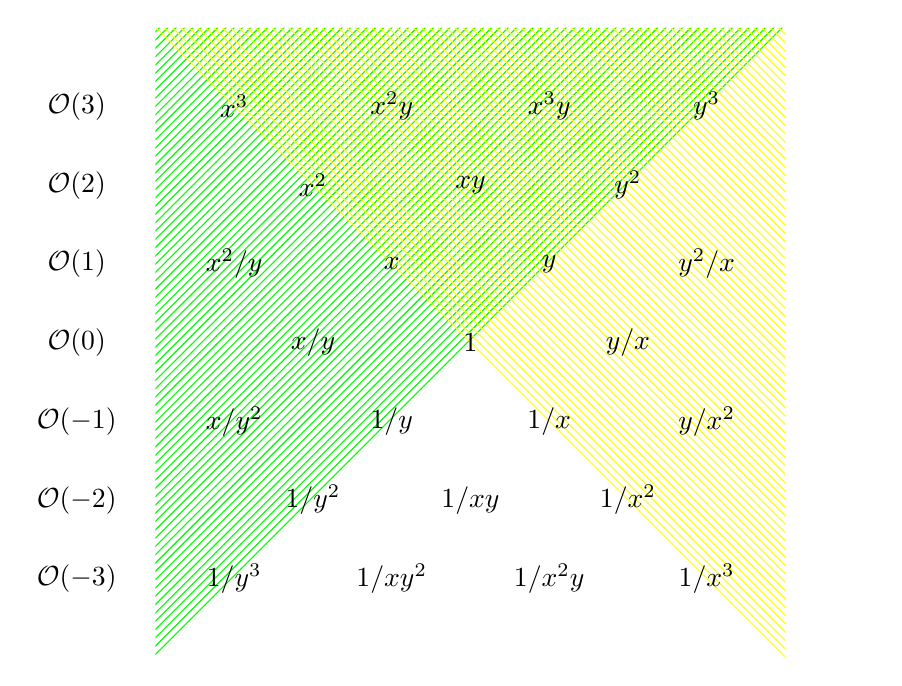
\begin{tikzpicture}
%    \foreach\ang in {60,120,...,360}{
%     \draw[->,blue!80!black,dotted] (0,0) -- (\ang:3cm);
%    }
%    \foreach\ang in {60,180, 300}{
%     \draw[->,black!80!black] (0,0) -- (\ang:1cm);
%    }

%    \draw[->,green!80!black,dotted] (-2,-2) -- (2,2);
%    \draw[->,yellow!80!black,dotted] (2,-2) -- (-2,2);
    \fill[pattern=north east lines, pattern color=green]    (-4,-4) -- (4,4) -- (-4,4) -- (-4,-4);
    \fill[pattern=north west lines, pattern color=yellow]    (4,-4) -- (-4,4) -- (4,4) -- (4,-4);
    \node at (0,0) {$1$};
    \node at (-1,1) {$x$};
    \node at (1,1) {$y$};
    \node at (1,-1) {$1/x$};
    \node at (-1,-1) {$1/y$};
    \node at (2,0) {$y/x$};
    \node at (-2,0) {$x/y$};
    \node at (3,1) {$y^2/x$};
    \node at (-3,1) {$x^2/y$};
    \node at (-3,-1) {$x/y^2$};
    \node at (3,-1) {$y/x^2$};
    \node at (0,2) {$xy$};
    \node at (2,2) {$y^2$};
    \node at (-2,2) {$x^2$};
    \node at (-2,-2) {$1/y^2$};
    \node at (2,-2) {$1/x^2$};
    \node at (0,-2) {$1/xy$};
    \node at (-3, -3) {$1/y^3$};
    \node at (-1,-3) {$1/xy^2$};
    \node at (1,-3) {$1/x^2y$};
    \node at (3,-3) {$1/x^3$};
    \node at (-3, 3) {$x^3$};
    \node at (-1,3) {$x^2y$};
    \node at (1,3) {$x^3y$};
    \node at (3,3) {$y^3$};
    \node at (-5,3) {$\OO(3)$};   
    \node at (-5,2) {$\OO(2)$};   
    \node at (-5,1) {$\OO(1)$};   
    \node at (-5,0) {$\OO(0)$};   
    \node at (-5,-1) {$\OO(-1)$};   
    \node at (-5,-2) {$\OO(-2)$};   
    \node at (-5,-3) {$\OO(-3)$};   
    \node at (5,3) {};   
    \node at (5,2) {};   
    \node at (5,1) {};   
    \node at (5,0) {};   
    \node at (5,-1) {};   
    \node at (5,-2) {};   
    \node at (5,-3) {};   
  \end{tikzpicture}
\end{center}

We wish to do the same for $\PP^2$; because of the increased dimension, we will draw each monomal degree one at a time.  Fix a basis $x, y, z$ of $V^*$, and a dual basis $x^\vee, y^\vee, z^\vee$ of $V$.  There are corresponding hyperplanes $H_x, H_y, H_z$ and corresponding opens $U_x, U_y, U_z$.  The half-planes $\sigma_x, \sigma_y, \sigma_z$ in the lattice will correspond to the opens $U_{yz}, U_{xz}, U_{xy}$.  Further, the opens $U_x, U_y, U_z$ will correspond to  the cones $\sigma_{yz} = \sigma_y \cap \sigma_z, \sigma_{xz}, \sigma{xy}$.

We will restrict ourselves to thinking about $H^0$ and $H^2$.  The student should interpret $H^0$ as the intersection of the cones $\sigma_{yz}, \sigma_{xz}, \sigma_{xy}$ and $H^2$ as the complement of the union of the cones $\sigma_x, \sigma_y, \sigma_z$.

This picture will be more complicated.  We let the below be our ``key.''  Those familiar will notice the root system for $SL_3$ or $GL_3$ appearing as the allowed ``lattice shifts.''  We will draw the cones $\sigma_x$ (green) and $\sigma_{yz}$ (yellow).  Note that this lattice has period 3; we can see this because the smallest degree monomial that lands back on top of the center $1$ is $xyz$, explaining the ``gap'' between $\OO(0)$ and $\OO(-3)$.
\begin{center}

  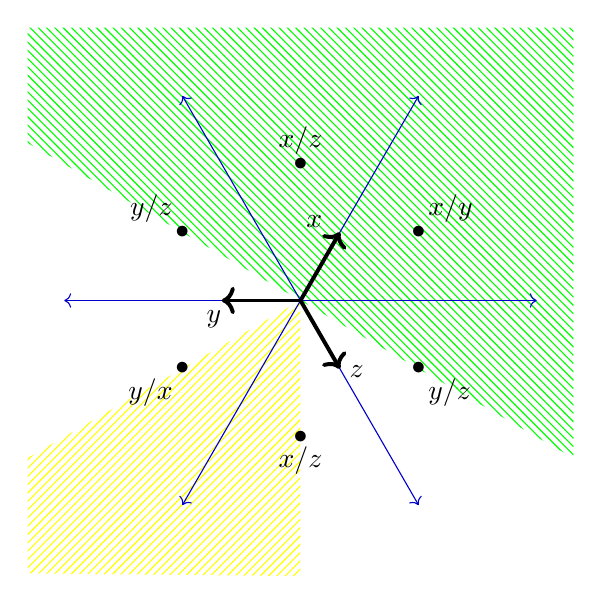
\begin{tikzpicture}
 
    \fill[pattern=north west lines, pattern color=green]    (0,0) -- (-30:4cm) -- (45:4.9cm) -- (135:4.9cm) -- (150:4cm); 
    
        \fill[pattern=north east lines, pattern color=yellow]    (0,0) -- (-150:4cm) -- (-135:4.9cm) -- (-90:3.5cm) -- (0,0); 
 
    \foreach\ang in {60,120,...,360}{
     \draw[->,blue!80!black] (0,0) -- (\ang:3cm);
    }
    \foreach\ang in {60,180, 300}{
     \draw[->,black!80!black, line width=0.5mm] (0,0) -- (\ang:1cm);
    }
    \node[anchor=east] at (.4,1) {$x$};
    \node[anchor=north] at (-1.1,0) {$y$};
    \node[anchor=south west] at (.5,-1.1,0) {$z$};
    \node at (30:1.732cm) {$\bullet$};
    \node[anchor=south west] at (30:1.732cm) {$x/y$};
    \node at (-30:1.732cm) {$\bullet$};
    \node[anchor=north west] at (-30:1.732cm) {$y/z$};
    \node at (-90:1.732cm) {$\bullet$};
    \node[anchor=north] at (-90:1.732cm) {$x/z$};
    \node at (-150:1.732cm) {$\bullet$};
    \node[anchor=north east] at (-150:1.732cm) {$y/x$};
    \node at (150:1.732cm) {$\bullet$};
    \node[anchor=south east] at (150:1.732cm) {$y/z$};
    \node at (90:1.732cm) {$\bullet$};
    \node[anchor=south] at (90:1.732cm) {$x/z$};    
\end{tikzpicture}
\end{center}
%
%Let us show $\OO(1)$ and $\OO(2)$.
%\begin{center}
%
%  \begin{tikzpicture}
% 
%%    \fill[pattern=north west lines, pattern color=green]    (0,0) -- (-30:4cm) -- (45:4.9cm) -- (135:4.9cm) -- (150:4cm); 
%    
%        \fill[pattern=north east lines, pattern color=yellow]    (60:1cm) -- +(-150:4cm) -- +(-135:4.9cm) -- +(-90:3.5cm) -- (60:1cm); 
% 
%    \foreach\ang in {60,120,...,360}{
%     \draw[->,blue!80!black] (0,0) -- (\ang:3cm);
%    }
%    \foreach\ang in {60,180, 300}{
%     \draw[->,black!80!black, line width=0.5mm] (0,0) -- (\ang:1cm);
%    }
%    \node[anchor=east] at (.4,1) {$x$};
%    \node[anchor=north] at (-1.1,0) {$y$};
%    \node[anchor=south west] at (.5,-1.1,0) {$z$};
%    \node at (30:1.732cm) {$\bullet$};
%    \node[anchor=south west] at (30:1.732cm) {$x/y$};
%    \node at (-30:1.732cm) {$\bullet$};
%    \node[anchor=north west] at (-30:1.732cm) {$y/z$};
%    \node at (-90:1.732cm) {$\bullet$};
%    \node[anchor=north] at (-90:1.732cm) {$x/z$};
%    \node at (-150:1.732cm) {$\bullet$};
%    \node[anchor=north east] at (-150:1.732cm) {$y/x$};
%    \node at (150:1.732cm) {$\bullet$};
%    \node[anchor=south east] at (150:1.732cm) {$y/z$};
%    \node at (90:1.732cm) {$\bullet$};
%    \node[anchor=south] at (90:1.732cm) {$x/z$};    
%\end{tikzpicture}
%\end{center}

The reader is encourage to try to doodle out the cones for $\OO(r)$, where $r=-4,-3,-2,-1,0,1,2,3$.  As we increase $r$, the yellow and green cones move toward each other.  We find that $H^0(\PP(V), \OO(r))$ corresponds to the weight diagram for $\Sym^k V^*$, and $H^2(\PP(V), \OO(-3-r)$ corresponds to the weight diagram for $\Sym^k V$.  \footnote{This is not an accidental phenomenon; $\PP^n$ is an example of a partial flag variety, and Serre duality is a degenerate case of Borel-Weil-Bott.  In Lurie's proof of Borel-Weil-Bott he uses Serre duality in an essential way to compute higher cohomologies.  The student may observe that the vertex of the cones lie on the reflection hyperplanes of the weight lattice, and changing $r$ corresponds to moving them along these hyperplanes.}  In the above example, if we examine only the $T$-weights, we find strong evidence that $H^n(\PP^2, \OO(-3-r))$ should be identified with $\Sym^r V$, but note that $GL_n$ does not act on $H^n(X, \OO(-n-1-r))$.  Note that $N(T)$ \emph{does} act, with $T$ acting by the weights pictured and the symmetric group $W = N(T)/T = S_{n+1}$ acting by reflecting across hyperplanes.


Now, let us discuss the general case.  What I would like to draw attention to now is the appearance of the dual space $(V^*)^* = V$.  This is quite odd; it is clear from the exercise that the $GL_n$ action on $V^*$ will induce the corresponding $GL_n$ action on $H^0(X, \OO(r)) = \Sym^r V^*$.  But it's not clear how this works for $H^n(X, \OO(-n-1-r))$ since it depends on a choice of Cech cover.  This choice can be formulated in the following equivalent ways:
\begin{itemize}
\item by choosing hyperplanes $H_0, \ldots, H_n$,
\item by choosing a basis of $V^*$ up to scaling,
\item by choosing a maximal torus $T \subset GL_{n+1}$,
\item by choosing a polynomial $k[V]$-subalgebra of $K = \Frac(k[V])$ with $\dim(V)$ generators,
\end{itemize}
which all admit compatible actions by change of basis $g \in GL_{n+1}$, but which are not $GL_{n+1}$-invariant.  However, they are $N(T)$-invariant and one can observe that the action of $N(T)$ on $H^n(X, \OO(-n-1-r))$ corresponds to the dual representations $\Sym^r V^*$.

%The point is that our lattice was obtained by choosing a basis of $V^*$, sometimes one defines \emph{lattice} in $K = \Frac(k[V])$, i.e. a finitely generated subring of $K$ containing the ``ring of integers'' $k[V]$, and it is only this subring that our lattice can see.  However, at the very least, we can observe that scaling acts on the ``bottom'' of the lattice via reciprocals, consistent with the idea that $H^n(X, \OO(-n-1-r))$ should be some kind of dual.   

Let us understand the residue map in this presentation.  A choice of sign of the ordering of the $x_i$ determines an isomorphism $\det(\Omega^1_{X/k}) \simeq \OO(-n-1)$.  %An element of $H^n(\PP(V), \OO(-n-1))$ may be understood, given a fixed choice of basis $x_0, \ldots, x_n$, as a multiple of the degree 0 monomial $x_i^n (x_0^{-1} \cdots x_{i-1}^{-1} x_{i+1}^{-1} \cdots x_n^{-1})$, and the residue simply takes the coefficient of this monomial.  This description naturally biases a choice of $i$, and corresponds geometrically to taking the residue at $p_i$.  Or, more invariantly, we can take a multiple of the degree $-n-1$ monomial $(x_0 \cdots x_n)^{-1}$.  
This defines a perfect pairing
$$H^0(X, \OO(r)) \otimes_k H^n(X, \OO(-n-1-r)) \rightarrow k$$
as follows.  We have that $H^0(X, \OO(r))$ consists of $\Sym^r V$, i.e. degree $r$ monomials of $V$.  On the other hand, $H^n(X, \OO(-n-1-r))$ consists of the span of degree $-n-r-1$ monomials modulo those where one of the $x_i^{-1}$ do not appear.  The natural multiplitcation map yields a monomial of degree $-(n+1)$, to which we take the coefficient of $x_0^{-1} \cdots x_n^{-1}$.  Note that monomials we killed in $H^n(X, \OO(-n-1-r))$ were those in which there was an $x_i^{-1}$ which did not appear, corresponding to functions holomorphic in the variable $x_i$.  Finally, we note that a change of basis $g$ will move the hyperplanes $H_0, \ldots, H_n$ as well as permute them (thus twisting the identification with $\det(\Omega^1_{X/k})$) in a compatible way, thus concluding
$$H^n(X, \OO(-n-1-r)) = \Sym^r V.$$
\end{proof}

The above verifies Serre duality for $\PP^n_k$ for line bundles.  We now extend it to all coherent sheaves.
\begin{prop}
For any coherent sheaf $\mathcal{F}$ on $\PP^n_k$, the natural map
$$\Ext^{n-i}(\OO_X, \mathcal{F}) \otimes \Ext^i(\mathcal{F}, \omega_X) \rightarrow \Ext^n(\OO_X, \mathcal{F}) \rightarrow k$$
is a perfect pairing.
\end{prop}
\begin{proof}
We have shown that the pairing is perfect for vector bundles, as well as functorial for maps between them.  Using the resolution property for $\PP^n$, there is a finite sequence of short exact sequences
$$0 \rightarrow \mathcal{K}_{j+1} \rightarrow \mathcal{E}_j \rightarrow \mathcal{K}_j \rightarrow 0$$
where the $\mathcal{E}_j$ are sums of line bundles, and for the top index $m$, we have $\mathcal{K}_{m} = \mathcal{E}_{m}$, and for the bottom index we have $\mathcal{K}_0 = \mathcal{F}$.  Now, we can form the associated long exact sequences for $\Ext^{n - \bullet}(\OO_X, -)^\vee$ and $\Ext^\bullet(-, \omega_X)$ and apply the five-lemma to the final short exact seqeunce to get an equivalence for input $\mathcal{K}_{m-1}$.  Continuing in the same fashion, we obtain the desired equivalence for input $\mathcal{F}$.
\end{proof}


Finally, let us prove the strongest form of Serre duality.
\begin{prop}
Let $f: X = \PP^n_k \rightarrow \Spec k$.  Define $\omega_X = \det(\Omega^1_X)[n]$, and define a functor
$$f^! V = f^* V \otimes_{\OO_X} \omega_X.$$
Then, there is an adjunction $(Rf_*, f^!)$.
\end{prop}
\begin{proof}
First, note that the naive dual $(-)^\vee: k\dmod \rightarrow k\dmod$ is exact, and defines a functor $(-)^\vee: D(k) \rightarrow D(k)$ on derived categories.  Note that both $Rf_*$ and $f^!$ are well-defined on $D^b(\Coh(X))$ and $D^b(\Coh(\Spec k))$; that is, we wish to produce a functorial equivalence
$$(Rf_* \mathcal{F})^\vee \otimes_k V \simeq \Hom_{D^b(\Coh(X))}(\mathcal{F}, f^*V \otimes_{\OO_X} \omega_X) = \Hom_{D^b(\Coh(X))}(\mathcal{F}, \omega_X) \otimes_k V$$
with the last equality following since $\Hom$ commutes with finite direct sums in both inputs.  We can thus take the case $V = k$.  In this case, the same argument above suffices since bounded coherent complexes also have finite resolutions.  Finally, Since $D(\QCoh(X)) = \Ind(D^b(\Coh(X))$ and likewise for $Y$, the adjunction on compact objects induces an adjunction on ind-completions\footnote{I.e. $\Hom(\colim X_i, \colim Y_j) = \lim_i \colim_j \Hom(X_i, Y_j)$, with the order mattering, since we can only commute the colimits for $X_i$ compact.}.
\end{proof}




\subsection{Formal aspects of Grothendieck duality}


Part of the modern approach to Grothendieck duality is pure formality; we discuss this aspect now.
\begin{thm}
Let $f: X \rightarrow Y$ be a finite-type morphism of Noetherian schemes.  Then functor $Rf_*: D(\QCoh(X)) \rightarrow D(\QCoh(Y))$ has a right adjoint, which we denote $f^\times$.  If, furthermore, $f$ has finite Tor-dimension, then the there is a natural isomorphism
$$\chi: Lf^*(-) \otimes^L_{\OO_X} f^\times \OO_Y \rightarrow f^\times.$$
Furthermore, the counit morphism $\epsilon$ can be generally computed in terms of the counit $Rf_* f^\times \OO_Y \rightarrow \OO_Y$ via the diagram
$$\begin{tikzcd}
Rf_*(Lf^*(-) \otimes^L_{\OO_X} f^\times \OO_Y) \arrow[d, "\chi"] & - \otimes^L Rf_* f^\times \OO_Y \arrow[l, "\pi"] \arrow[r, "\epsilon"] & - \otimes_{\OO_Y} \OO_Y \arrow[d, equals] \\
Rf_* f^\times(-) \arrow[rr, "\epsilon"] & & -
\end{tikzcd}$$
where $p$ denotes the projection formula equivalence.
\end{thm}


\begin{rmk}
In general, $f^\times$ does not come from the derived functor of a functor on abelian categories.
\end{rmk}

\begin{rmk}
The functor $f^\times$ is most often considered when $f$ is proper, in which case we denote it by $f^!$ per the discussion above.  When $f$ is not proper, the behavior of $f^\times$ can be rather mysterious.
\end{rmk}

\begin{exmp}
Taking $j: \G_m = \Spec k[x,x^{-1}] \rightarrow \mathbb{A}^1 = \Spec k[x]$, we have that $j^*(M)$ is the coinduction, i.e. the quotient by $x$-torsion, while $j^\times(M)$ is the $x$-divisible sub-module.
\end{exmp}

%\begin{exmp}
%Taking $j: \mathbb{A}^2 - \{0\} \rightarrow \mathbb{A}^2 = \Spec k[x,y]$, \todo{????}
%\end{exmp}


%\begin{rmk}
%One can remove the Tor-finiteness condition by working in the category $\IndCoh(X)$ rather than $\QCoh(X)$.  This category is somewhat mysterious; on the other hand, if one is only interested in coherent sheaves $D^b(\Coh(X))$ and one shows that $f^!
%\end{rmk}



Now, we come to the adjoint functor theorem.  We begin with the following disclaimer: the following adjoint functor theorem is ``not good enough'' for us.  The reason is that for us, the categories are not merely categories but triangulated categories where the naive notion of colimit is the wrong one.  Instead, one should consider \emph{homotopy} colimits, which still don't exist, but which can be approximated.  Namely, suppose we are in a triangulated category with all coproducts; every colimit can be written via coproducts and coequalizers.  The homotopy coequalizer of $(f, g): X \rightarrow Y$ in a triangulated category ``should be'' $\cone(f - g)$, and we can declare this so by fiat, although cones do \emph{not} satisfy the usual universal property, and therefore are not honest colimits in any sense (recall that cones are not functorial in a triangulated category)!

It is possible to prove an adjoint functor theorem in the triangulated setting, but it takes some work (see Theorem 4.1 in \cite{Neeman:GDBR}).  But there is a more ``modern approach'' which is in some sense cleaner, and a more direct generalization of the classical adjoint functor theorem.  This is the $\infty$-adjoint functor theorem for $(\infty, 1)$-categories, which unfortunately takes us too far afield.

We will prove the classical adjoint functor theorem; the $\infty$-analogue is argued in a similar way, but the set-up takes some time.
\begin{thm}[Classical adjoint functor theorem]
Let $F: \cat{C} \rightarrow \cat{D}$ be a functor of locally presentable\footnote{A category is \emph{locally presentable} if is locally small (hom-sets are sets not classes), admits all small colimits, and is accessible.  A category is \emph{accessible} if there is a cardinal $\kappa$ such that the category has $\kappa$-filtered colimits and if there is a set (not a class) of $\kappa$-compact objects that generate the category under $\kappa$-filtered colimits.} categories.  Then, $F$ has a right adjoint adjoint if and only if commutes with small colimits.  Furthermore, if $F$ preserves $\kappa$-compact objects, then its right adjoint also commutes with small colimits.
\end{thm}
\begin{proof}
Let us sketch the idea of the proof.  The forward direction is an exercise.  For the backwards direction, the idea is the following: if $F$ had a right adjoint $G$, then we would have $\Hom_{\cat{D}}(F-, Y) = \Hom_{\cat{C}}(-, GY)$.  This idea is to give a way to reconstruct an object from the category of morphisms into it -- a kind of categorical Brown representability.

Let $Y$ be a $\kappa$-compact object.  Take $I_Y$ to be the category with objects $\{(X, f) \mid X \in \cat{C}^\kappa, f: FX \rightarrow Y\}$ and the obvious morphisms -- since the categories are accessible, this is a small category.  We define, using the fact that small colimits exist in $\cat{C}$,
$$G(Y) = \colim_{(X, f) \in I_Y} X.$$
Given this, we have for compact $X$,
$$\Hom_{\cat{C}}(X, GY) = \Hom_{\cat{C}}(X, \colim_{(X', f) \in I_Y} X') = \colim_{(X', f) \in I_Y} \Hom_{\cat{C}}(X, X') = \Hom(X, FY)$$
with the last equality following by the tautological fact that every map $X \rightarrow X'$ factors through the identity on $X$.  The functor $G$ can be extended to $\cat{D}$ by ind-completion.
\end{proof}

This is not enough, however.  We need to know that the adjoint functor is also triangulated.  The most modern way to approach this is using $\infty$-categories, i.e. to use an $\infty$-categorical adjoint functor theorem, but this is beyond our scope.  We state the version for triangulated categories.
\begin{prop}[Adjoint functor theorem for triangulated categories]
Let $F: \cat{C} \rightarrow \cat{D}$ be a triangulated functor of triangulated categories, where $\cat{C}$ is compactly generated.  Further assume that $F$ commutes with coproducts.  Then, $F$ has a right adjoint $G$ (which must also be triangulated).  Further, let $S$ be a generating set for $\cat{C}$; then $G$ commutes with coproducts if and only if $F$ takes $S$ to compact objects of $\cat{D}$.
\end{prop}




There are a few less formal results we need form algebraic geometry.
\begin{prop}
Let $X$ be a quasicompact and quasiseparated scheme.  Then, $D_{qc}(X)$ is compactly generated, and the compact objects are $\Perf(X)$.
\end{prop}
\begin{proof}
See the Stacks Project, Lemma 35.16.2 and Theorem 35.14.3.
\end{proof}

\begin{prop}
Let $f: X \rightarrow Y$ be a quasicompact separated morphism of schemes.  Then $f_*: D(\QCoh(X)) \rightarrow D(\QCoh(Y))$ commutes with colimits.
\end{prop}
\begin{proof}
Again, this is confusing due to our cheating.  In the triangulated setting, we really want $Rf_*$ to be exact (automatic) and for it to commute with direct sums, which is easy to verify via the Cech complex.
\end{proof}

\begin{rmk}
The above is false if $f$ is not quasicompact.  For example, let $S$ be an infnite set take $f: X = \coprod_S \Spec k \rightarrow Y = \Spec k$.  Then, $\QCoh(X)$ consists of a collection of vector spaces $V$ indexed by $S$, and $f_* V = \prod_{s \in S} V_s$.  Since one cannot commute infinite direct sums and direct products, $f_*$ does not commute with colimits.
\end{rmk}




The consequence is the following definition.
\begin{defn}
Let $f: X \rightarrow Y$ be a quasicompact quasiseparated morphism of schemes.  The \emph{relative dualizing complex} is defined to be $\omega_f = f^! \OO_Y$.
\end{defn}

\begin{exmp}
If $f: \PP^n_k \rightarrow \Spec k$, then $\omega_f \simeq \det(\Omega^1_{\PP^n_k/k})[n]$.
\end{exmp}



\subsection{Exceptional pullback for closed embeddings}

Let us treat the affine case first.  A map of rings $\phi: B \rightarrow A$ induces a proper map of schemes if and only if it is a closed embedding; so take $A = B/I$.  Let $i: X = \Spec(A) \rightarrow Y = \Spec(B)$.  The functor $f_* = \phi^*$ is the restriction of scalars functor.

\begin{prop}
The restriction of scalars has a left adjoint, called the coinduction
$$i^* M = \phi_! M = M \otimes_B A$$
and a right adjoint, called the induction
$$i^! M = \phi_* M = \Hom_B(A, B).$$
\end{prop}

This construction sheafifies.
\begin{defn}
Let $i: Z \hookrightarrow X$ denote a closed embedding.  Then, there is a functor $i^!: D_{qc}(\OO_X) \rightarrow D_{qc}(\OO_Z)$ defined by
$$i^!(\mathcal{F}) = i^{-1}R\shHom_{\OO_X}(i_* \OO_Z, \mathcal{F}).$$
This functor is right adjoint to the functor $Ri_* = i_*$.
\end{defn}

\begin{exmp}
If $X$ has the resolution property, i.e. every quasicoherent sheaf has a locally $\mathcal{F}$ free resolution $\mathcal{E}^\bullet$, then we can write
$$i^! \mathcal{F} = i^{-1} \shHom_{\OO_X}(\mathcal{E}^\bullet, \mathcal{F}).$$
If $\mathcal{F}$ is coherent, then we can further write this as $i^{-1}((\mathcal{E}^\bullet)^\vee \otimes_{\OO_X} \mathcal{F})$.
\end{exmp}


\begin{prop}
Let $X$ be a smooth variety of dimension $n$ over $k$, and $i: Z \hookrightarrow X$ a regular embedding of codimension $r$.  Then, there is a natural identification
$$i^!(\mathcal{F}) \simeq \det(\mathcal{N}_{Z/X}) \otimes_{\OO_Z} i^* \mathcal{F}[-r].$$
In particular, 
$$\omega_Z = i^! \omega_X \simeq \det(\mathcal{N}_{Z/X}) \otimes_{\OO_Z} \omega_X|_Z[-r].$$
\end{prop}
\begin{proof}
Since $i$ is regular, it is Tor-finite.  So by the theorem, we can study $\mathcal{F} = \OO_X$.  We claim there is a quasi-isomorphism
$$i^{-1}R\shHom_{\OO_X}(i_*\OO_Z, \OO_X) \rightarrow \det(\mathcal{N}_{Z/X})[-r].$$
Let us define it affine locally in a canonical way.  Affine locally, we can take $X = \Spec R$ and $Z = \Spec R/I$ where $I = (f_1, \ldots, f_r)$ is a regular sequence.  

Let $K^\bullet = K^\bullet(R; f_1, \ldots, f_r)$ be the Koszul resolution; term-wise, it can be written as $R \otimes_k \bigwedge^i V$ where $V$ be the formal $k$-linear span of symbols $\epsilon_1, \ldots, \epsilon_r$, with the differential sending $\epsilon_i \mapsto f_i$.  Affine locally, note that
$$R\Hom_R(R/I, R) = \Hom_R(K^\bullet, R) = (K^\bullet)^\vee \twoheadrightarrow R/I \otimes_k \bigwedge^r V^*[-r].$$
Now, we claim the right hand side is canonically identified with $\det(I/I^2)^\vee$.  This follows from the fact that there is a map $R/I \otimes_k V \rightarrow I/I^2$ which is independent of the choice of generators $f_1, \ldots, f_r \in I$ in the sense that if we choose generators $g_1, \ldots, g_r$ corresponding to a vector space $W$, then the matrix $A$ with coefficients in $R$ relating the two generators induces a map $R/I \otimes V \rightarrow R/I \otimes W$ which commutes with the maps to $I/I^2$ (we leave the details as an exercise).
\end{proof}

\begin{rmk}
We leave it to the reader to work out what the trace is.
\end{rmk}

\begin{exmp}
The reader is encouraged to work out the case of a hypersurface  $X$ of degree $d$ in $\PP^n_k$, which is cut out by a section of $\OO(d)$, and verify that $\omega_X \simeq \OO(-n-1+d)|_X$.
\end{exmp}

\begin{rmk}
In particular, if $X \hookrightarrow \PP^n_k$ is smooth, then it is automatically lci.  Furthermore, by the usual exact sequence we have an identification $\det(\Omega^1_X) \simeq \det(\Omega^1_{\PP^n_k}) \otimes_{\OO_X} \det(\mathcal{N}_{X/\PP^n_k})$, so we have the following.
\end{rmk}

\begin{prop}
Let $X$ be a smooth projective scheme over $k$.  Then, $f^!(-) \simeq f^*(-) \otimes_{\OO_X} \det(\Omega^1_{X/k})[n]$.
\end{prop}


Finally, let us state Grothendieck duality, although we will not prove it.
\begin{thm}[Grothendieck duality]
Let $f: X \rightarrow Y$ be a smooth and proper morphism of relative dimension $d$.  Then, there is an isomorphism $f^! \OO_Y \simeq \omega_{X/Y}[d]$.
\end{thm}

%%TODO IN THE FUTURE: Grotehndiecu duality for quasismooth???

%\begin{defn}
%We say a morphism of schemes $f: X \rightarrow Y$ is \emph{quasismooth} if for every $x \in X$, there is an affine neighborhood $U$ of $x$ such that $f|_U$ can be factored as a regular embedding \todo{koszul regular?} followed by a smooth morphism.
%
%\todo{equivalent to below?} https://stacks.math.columbia.edu/tag/068E
%, and an affine open $V = \Spec B \subset Y$ such that $U \subset f^{-1}(V)$, such that $U$ is an open subscheme of $W = \Spec B[x_1, \ldots, x_n]/(f_1, \ldots, f_r)$ with $f_1, \ldots, f_r$ a regular sequence.
%\end{defn}
%
%\begin{thm}
%If $f: X \rightarrow Y$ is quasismooth, then $f^! \OO_Y \simeq $ \todo{???}
%\end{thm}

\subsection{Grothendieck local duality}

Let us outline a few known results on the dualizing sheaf.  Let $f: X \rightarrow \Spec k$ be a proper morphism, where $k$ is a perfect field.
\begin{itemize}
\item If $X$ is smooth over $k$, then $\omega_f = \det(\Omega^1_{X/k})[\dim(X)]$.
\item If $X$ is Gorenstein, then $\omega_f = \LL[\dim(X)]$ for some line bundle $\LL$.
\item If $X$ is Cohen-Macaulay, then $\omega_f = \mathcal{F}[\dim(X)]$ for a coherent sheaf $\mathcal{F}$.
\end{itemize}

Let's recall what these words mean.
\begin{defn}
A Noetherian ring $R$ is a \emph{complete intersection} if it is the quotient of a regular local ring by a regular sequence, $R$ is \emph{Cohen-Macaulay} if the depth (the maximal length of a regular sequence) of $R$ is equal to its Krull dimension, and $R$ is \emph{Gorenstein} if $R$ has finite injective dimension\footnote{We say a complex $M^\bullet \in D(R)$ has \emph{injective amplitude} in $[a, b]$ if it is quasi-isomorphic to a complex of injectives supported in the cohomological range $[a, b]$.  It is a homological algebra exercise to show that $M^\bullet$ has injective dimension in $[a, b]$ if and only if $\Ext^i_R(N, M^\bullet) = 0$ for all $R$-modules $N$ and $i \not\in [a,b]$ if and only if the same statement holds for $N = R/I$.  The injective dimension of an $R$-module $M$ is the smallest $d$ such that $M$ has injective amplitude in $[0, d]$.  When $R$ is a finite-type algebra over a perfect field $k$, it suffices to test on maximal ideals $I = \mf{m}$.} as an $R$-module.
\end{defn}


\begin{defn}
Let $R$ be a Noetherian ring.  A finitely generated module $M$ is a \emph{dualzing module} if for any maximal ideal $\mf{m}$ of height $r$, there is a quasi-isomorphism $R\Hom_R(R/\mf{m}, M) \simeq k[-n]$.
\end{defn}

Let us phrase this geometrically.  The idea is although the functor $f^!$ cannot be computed affine locally, we can test the existence of a dualizing sheaf locally.  To simplify things (and because I'm not sure what happens more generally), let us take everything over a perfect field $k$.
\begin{defn}
Let $X$ be a scheme over a perfect field $k$.  We say that $\omega_X \in \Coh(X)$ is a \emph{dualizing module} if for any inclusion of a closed point $i: \{x\} \rightarrow X$ of codimension $r$ (which is, in particular, proper), we have a quasi-isomorphism 
$$R\Hom_{OO_X}(i_* \kappa(x), \omega_X) \simeq R\Hom_{\{x\}}(\kappa(x), i^!\omega_X) = \kappa(x).$$
since the composition $g: \{x\} = \Spec \kappa(x) \rightarrow X \rightarrow k$ is smooth of relative dimension 0 (as $k$ is perfect), so $g^! k = \kappa(x)$.
\end{defn}

Note that we did not insist that $X$ is affine; in fact we will mostly apply it to the case when $X$ is projective.  The point is that every $x \in X$ has an affine open neighborhood, so if we had a candidate for a dualizing sheaf $\omega_X$ then we could test it on affines.  In fact, we can test it on local rings, and assume that $R$ is a Noetherian local ring.

\begin{prop}
Let $R$ be a ring.  Then if $R$ is regular, then it is a complete intersection, then it is Gorenstein, then it is Cohen-Macaulay.
\end{prop}
%\begin{proof}
%A regular ring is a complete intersection by definition.  A complete intersection ring $R = Q/(f_1, \ldots, f_r)$ is Gorenstein, since 
%\end{proof}


\begin{prop}
Suppose that $R$ is a Cohen-Macaulay local ring of Krull dimension $n$.  Then $R$ has a dualizing module $M$.  If $R$ is Gorenstein local, then $M \simeq R$, and the injective dimension of $R$ is $n$.
\end{prop}


\begin{prop}
If $X$ is a projective Cohen-Macaulay scheme pure of dimension $n$ over a perfect field $k$, then $X$ has a dualizing sheaf, i.e. $p^! k = \omega_X[n]$ for a coherent sheaf $\omega_X$.
\end{prop}
\begin{proof}
The dualizing complex exists in a general situation; we only have to show it has injective amplitude $[n, n]$, which, since $X$ is over a perfect field $k$, we can check on local rings at maximal ideals.
\end{proof}


\newpage


\section{Riemann-Roch}


\subsection{Some history and generalizations}

\begin{rmk}
In 1857 Bernhard Riemann proved \emph{Riemann's inequality}: for a Riemann surface (alegbraic curve) of (topological) genus $g$, the inequality provides a sufficient condition to construct meromorphic functions with zeroes and poles of given order at given points.  In modern language this prescription can be described by a divisor $D$; let $L(D)$ denote the complete linear system corresponding to that divisor (i.e. subspace of meromorphic functions with poles of order no greater than as specified).  Riemann's inequality states that
$$\dim(L(D)) \geq \deg(D) + 1 - g$$
\end{rmk}

\begin{rmk}
In 1865, Riemann and his student Gustav Roch found the ``correction term'' which gave an equality
$$\dim(L(D)) - \dim(L(K - D)) = \deg(D) + 1 - g$$
where $K$ is the canonical divisor (the divisor of a global meromorphic 1-form, which are all linearly equivalent).
\end{rmk}

\begin{rmk}
In 1954, Friedrich Hirzebruch interpreted the Riemann-Roch theorem topologically for compact complex manifolds $X$ of any dimension.  Namely, for $E$ a vector bundle on $X$, we have
$$\chi(X, E) = \int_X \ch(E) \Td_X$$
where $\ch(E)$ is the \emph{Chern character} of the complex vector bundle $E$ and $\Td_X$ is the \emph{Todd class} of the variety $X$ (i.e. the Todd class associated to the tangent bundle of $X$).

For complex curves, Serre duality identifies the left-hand side of Riemann-Roch with the Euler characteristic
$$\dim(L(D)) - \dim(L(K-D)) = \chi(X, \mathcal{L}(D)).$$
The Todd class and Chern character for $\OO_X(D)$ are given by
$$\Td_X = 1 + \frac 1 2 c_1(TX), \;\;\;\;\;\;\; \ch(\OO_X(D)) = 1 + c_1(\OO_X(D))$$
so that the right-hand side reads
$$\int_X \frac 1 2 c_1(TX) + c_1(\OO_X(D)) = \frac 1 2 (2 - 2g) + \deg(D).$$
\end{rmk}

\begin{rmk}
Finally, in 1957, Grothendieck proved a generalization to smooth quasi-projective schemes over any field.  He replaces the singular cohomology with the \emph{Chow ring}\footnote{We write $A^k(X)$ to denote codimension $k$ cycles, so that the intersection product makes $A^\bullet$ a graded ring.} with rational coefficients\footnote{We only need rational coefficients to define the Chern character, since exponentials are involved.} $A^\bullet(X; \Q) = A^\bullet(X) \otimes_{\Z} \Q$ and defines an \emph{algebraic Chern character} $\ch: K^0(X) \rightarrow A^\bullet(X)$ from the category of algebraic vector bundles to the Chow group, and a \emph{cycle class map} $\mathrm{cl}_{\Q}: A^\bullet(X; \Q) \rightarrow H^\bullet(X; \mathbb{Q})$ to singular cohomology which just considers each algebraic cycle as a geometric chain.
\end{rmk}

\begin{thm}[Grothendieck-Riemann-Roch]
Let $X, Y$ be smooth quasi-projective schemes over a field, and let $f: X \rightarrow Y$ be a proper morphism.  Then, the following diagram commutes
$$\xymatrix{
K^0(X) \ar[r]^-{\ch  \cup \Td_X} \ar[d]_{f_!}  & A_\bullet(X)_\Q \ar@{=}[r] \ar[d]_{f_*} & A^\bullet(X)_\Q \ar[d]^{f_!}  \\
K^0(Y) \ar[r]_-{\ch \cup \Td_Y} & A_\bullet(Y)_\Q \ar@{=}[r] & A^\bullet(Y)_\Q
}$$
where $f_!$ is the map on $K$-groups induced by the derived pushforward $Rf_*$, and the usual pushforward for Chow cycles\footnote{The shriek $!$ is used to indicate that it is a surprising ``Gysin'' pushforward, i.e. on cohomology.  We get this via Poincar\'{e} duality.}.
\end{thm}

\begin{rmk}
What about if $X$ and $Y$ are singular?  We don't have Poincar\'{e} duality, so we can't even formulate what we want.  Replacing everything with ``covariant'' homology-type theories doesn't work either, because the Chern character is really defined on vector bundles.  This may serve as a motivation for the introduction of so-called ``bivariant theories.''  We will let $K^0 = K(\mathrm{Vect}(X))$ and $K_0 = K(\Coh(X))$.
\end{rmk}

\begin{thm}[Baum-Fulton-MacPherson-Grothendieck-Hirzebruch-Riemann-Roch]
Suppose either (a) $H$ denotes singular (co)homology with rational coefficients and $k = \C$, or $H$ denotes Chow (co)homology and $k$ is any field.  Let $X, Y$ be quasiprojective schemes over $k$.  There are unique natural transformations $\ch: K^0 \rightarrow H^\bullet$ and $\tau: K_0 \rightarrow H_\bullet$ satisfying the following properties:
\begin{enumerate}[(1)]
\item (naturality) for any proper morphism $f: X \rightarrow Y$, one has a commutative square
$$\xymatrix{
K_0(X) \ar[r]^\tau \ar[d]_{f_*} & H_\bullet(X) \ar[d]^{f_*}  \\
K_0(Y) \ar[r]_{\tau} & H_\bullet(Y)
}$$
and for any morphism $f: X \rightarrow Y$ one has a commutative square
$$\xymatrix{
K^0(Y) \ar[r]^\ch \ar[d]_{f^*} & H^\bullet(Y) \ar[d]^{f^*}  \\
K^0(X) \ar[r]_{\ch} & H^\bullet(X)
}$$


\item (cap product) for any variety $X$, the following diagram commutes
$$\xymatrix{
K^0(X) \otimes K_0(X) \ar[d]_-{\otimes} \ar[r]^{\ch \otimes \tau} & H^\bullet(X) \otimes H_\bullet(X)  \ar[d]^-\cap \\
K_0(X) \ar[r]_\tau  & H_\bullet(X)
}$$

\item (smooth case) if $X$ is smooth, then
$$\tau(\OO_X) = \Td_X \cap [X]$$
i.e. $\tau(\OO_X)$ is the homology Todd class obtained under Poincare duality.  Using (2) one has further that
$$\tau(\mathcal{E}) = \ch(\mathcal{E}) \cap \Td_X$$
for a vector bundle $\mathcal{E}$. 
\end{enumerate}
\end{thm}

%\begin{rmk}
%If $X, Y$ are smooth, then property (1), along with the last formula from property (3) (which uses property (2)), is the classical Riemann-Roch theorem.
%\end{rmk}



\subsection{Riemann-Roch for regular projective curves}

Let's prove Riemann-Roch.  With modern machinery, it will not take us long.

\begin{defn}
Let $X$ be a proper scheme over a field $k$, and $\mathcal{F} \in \Coh(X)$.  We adopt the notation
$$h^i(X, \mathcal{F}) := \dim_k(H^i(X, \mathcal{F})).$$
We define the \emph{Euler characteristic} by
$$\chi(X, \mathcal{F}) := \sum_{i=0}^{\dim X} (-1)^i h^i(X, \mathcal{F}).$$
\end{defn}

\begin{exmp}
We have that
$$\chi(\PP^n_k, \OO(r)) = \binom{n+r}{r}.$$
Note the absence of cases in the description of the Euler characteristic, as opposed to the cases involved in $h^0$ and $h^n$.
\end{exmp}




\begin{thm}[Riemann-Roch]
Let $X$ be a smooth projective scheme of dimension 1 (i.e. a projective curve), and $\mathcal{L}$ a line bundle on $X$.  Then we have
$$\chi(X, \mathcal{L}) = \chi(X, \OO_X) + \deg(\mathcal{L}).$$
\end{thm}
\begin{proof}
We leave it as an exercise to show that the Euler characteristic is additive in short exact sequences.  Suppose $\mathcal{L} \simeq \OO_X(D)$ for some Weil divisor $D$.  Choose a closed point $x \in X$ and let $D' = D + [x]$.  There is a short exact sequence
$$0 \rightarrow \OO_X(D) \rightarrow \OO_X(D') \rightarrow k_x \rightarrow 0$$
Note that $\chi(k_x) = 1$, so we have
$$\chi(\OO_X(D')) = \chi(\OO_X(D)) + 1$$
which proves 
\end{proof}

\begin{defn}
Let $X$ be a smooth projective variety over a field $k$.  We define the \emph{geometric genus} of $X$ to be (the equality coming from Serre duality)
$$\rho_g(X) := h^0(X, \det(\Omega^1_{X/k}) = h^1(X, \OO_X).$$
\end{defn}

\begin{cor}
For curves, the geometric genus is equal to the arithmetic genus.
\end{cor}



\begin{rmk}
Let $g = \rho_g(X)$.  Riemann Roch also comes in the form
$$\dim(L(D)) - \dim(L(K-D)) = \deg(D) + 1 - g.$$
\end{rmk}


%\subsection{What does Riemann-Roch tell us about line bundles on curves?}
%
%There are two invariants we assign to a line bundle $\LL$ on a curve $X$: $h^0$ is the number of global sections, and $h^1$ is something else; but Serre duality tells us that $h^1(X, \LL) = h^0(X, \LL^\vee \otimes_{\OO_X} \omega_X)$.  Let us first establish the following two results which do not use Riemann-Roch.

Let us recall the following.
\begin{prop}
If $\deg(\mathcal{L}) < 0$, then $h^0(X, \mathcal{L}) = 0$.  If $\deg(\LL) = 0$, then $h^0(\LL) = 0$ or $\LL \cong \OO_X$.
\end{prop}
%\begin{proof}
%If $\LL$ has a global section, then it defines an effective Weil divisor $D$.  But then, $\LL \simeq \OO_X(D)$, so $\deg(\LL) \geq 0$.
%\end{proof}


%\begin{proof}
%Suppose $\deg(\LL) = 0$ and $\LL$ has a nonzero global section.  Since the Weil divisor it defines must be degree 0, this section has no zeroes.  A section with no zeroes generates $\OO_X$.
%\end{proof}
%%
%%\begin{exmp}[Degree 0 line bundle with no global sections]
%%$\mathcal{O}(P - Q)$ on an elliptic curve.
%%\end{exmp}
%
Now, some corollaries of Riemann-Roch.

\begin{cor}
We have $\deg(K) = 2g - 2$.
\end{cor}
\begin{proof}
Apply Riemann-Roch with $D = K$ and $D = 0$.
\end{proof}
%
%
\begin{cor}
If $\deg(\LL) = 2g-2$, then either $\mathcal{L} \cong \omega_X$ and $h^0(X, \LL) = g$ or $h^0(X, \LL) = g-1$.  If $\deg(\LL) > \deg(\omega) = 2g - 2$, then $h^1(\mathcal{L}) = 0$ and $h^0(\mathcal{L}) = 1 - g + \deg(\LL)$
\end{cor}
%\end{cor}
%\begin{proof}
%%This follows from that $\deg(\omega) = 2g - 2$, so in this case $\deg(\LL) < 0$.
%By Serre duality, $\deg(\mathcal{L}^\vee) < \deg(\OO_X) = 0$, so $h^1(X, \mathcal{L}) = 0$.  Using Riemann Roch, the result follows.
%\end{proof}
%
%\begin{cor}
%For any line bundle, changing the degree by one can change the number of global sections by at most one, i.e.
%$$\h^0(X, \mathcal{L}) - h^0(X, \LL(-P)) = 0, 1$$
%\end{cor}
%\begin{proof}
%Take the short exact sequence
%$$0 \rightarrow \OO(-P) \rightarrow \OO \rightarrow \C|_{P} \rightarrow 0$$
%Tensor by $\LL$, and take global sections, which is left-exact, to get
%$$0 \rightarrow H^0(X, \LL(-P)) \rightarrow H^0(X, \LL) \rightarrow H^0(X, \LL_P)$$
%So, $h^0(X, \LL) - h^0(X, \LL(-P)) = 0, 1$.
%\end{proof}0
%
%\begin{prop}
%If for all $P$, $h^0(X, \LL) - h^0(X, \LL(-P)) = 1$, then $\LL$ is base-point free.  If for all $P, Q$ (possibly equal), $h^0(X, \LL) - h^0(X, \LL(-P-Q)) = 2$, then $\LL$ is very ample.
%\end{prop}
%\begin{proof}
%For the first assertion, what this means is that there is a global section of $\LL$ which does not vanish at $P$.  Thus $\LL$ is base-point free.
%
%For the second, what this means is that there is a section vanishing at $P$ but not $Q$, so we have separation of points.  Now let $P = Q$; then there is a section which vanishes with order 1 but not 2.  Intuitively, it gives a hyperplane which is tangent to $P$, and since we are one a curve (one dimensional), and so the cotangent map is surjective.  More rigorously, the section gives a nonzero element of $\mf{m}_P\LL/\mf{m}_P^2 \LL$.
%\end{proof}

\begin{exmp}
Work out how much you can deduce from Riemann Roch about $h^0$ and $h^1$ of degree $d$ line bundles on genus $g$ curves.  As $g$ grows, you know less and less.
\end{exmp}

\subsection{Riemann-Roch for integral (possibly singular) curves}


\begin{defn}
Let $X$ be an integral curve over a field $k$ with generic point $\xi$, and $\mathcal{F} \in \Coh(X)$.  We define the \emph{rank} by
$$\rk(\mathcal{F}) = \dim_{\OO_{X, \xi}}(\mathcal{F}_\xi).$$
If $X$ is also projective, we define the \emph{degree} by 
$$\deg(\mathcal{F}) = \chi(X, \mathcal{F}) - \rk(\mathcal{F}) \cdot \chi(X, \OO_X).$$
We define the \emph{arithmetic genus} by
$$\rho_a(X) = 1 - \chi(X, \OO_X).$$
\end{defn}

\begin{rmk}
Although we can define degree in this way for a non-curve, it is not the right thing.  For example, for $X = \PP^2_k$, $\chi(X, \OO(n)) - 1 \neq n$.  The definition generalizes if we replace $\chi$ with the $(n-1)$th coefficient of the Hilbert polynomial:
$$\deg(\mathcal{F}) := \alpha_{n-1}(\mathcal{F}) - \rk(\mathcal{E}) \cdot \alpha_{d-1}(\OO_X)$$
where $\alpha_i$ is the $i$th coefficient of the Hilbert polynomial, and $\rk(\mathcal{F}) = \alpha_n(\mathcal{F})/\alpha_n(\OO_X)$.  Note that when $n=1$, i.e $X$ is a curve, $\alpha_0(\mathcal{F}) = \chi(X, \mathcal{F})$.  %  \todo{work out} Using Hirzebruch-Riemann-Roch, we have $\deg(\mathcal{F}) = c_1(\mathcal{F}) \cdot H^{d-1}$ where $H$ is an ample divisor.% \todo{??? hilbert functions postpone}
\end{rmk}

We leave the following as an exercise.
\begin{prop}
The Euler characteristic, rank, and degree are additive in short exact sequences.
\end{prop}

This allows us to compute the arithmetic genus using the normalization.
\begin{exmp}
Let $X$ be a singular curve, with singular points $x_1, \ldots, x_r$ and $\pi: \tilde{X} \rightarrow X$ the normalization.  There is a short exact sequence
$$0 \rightarrow \mathcal{O}_X \rightarrow \pi_* \mathcal{O}_{\widetilde{X}} \rightarrow \bigoplus_{i=1}^r \tilde{\OO_{p_i}}/\OO_{p_i} \rightarrow 0$$
where $\widetilde{\OO_{p_i}}$ is the integral closure.  In particular, we have
$$\rho_a(X) = \rho_a(\tilde{X}) + \sum_{i=1}^r \ell(\tilde{\OO_{p_i}}/\OO_{p_i})$$
where $\ell$ denotes the length of the module (note the sign).
\end{exmp}

There is another way to see arithmetic genus by degeneration in families.  
\begin{rmk}
Euler characteristic (and therefore genus) is constant in flat families.  We will prove a more general statement later: that Hilbert functions are constant in flat families.
\end{rmk}

\begin{exmp}
There is a family of elliptic curves depending on parameters $t_1, t_2$:
$$y^2 = x(x-t_1)(x-t_2)$$
which can degenerate by taking $t_1 = t_2 = 0$ (cuspidal curve) or by taking $t_1 = t_2 \ne 0$ (nodal curve).
\end{exmp}




The following is now tautological.
\begin{thm}[Riemann-Roch]
Let $X$ be an integral scheme over a field $k$, and $\mathcal{F} \in Coh(X)$.  Then, we have
$$\chi(X, \mathcal{F}) = \chi(X, \OO_X) + \deg(\mathcal{F}).$$
Furthermore, if $X$ is a local complete intersection with canonical sheaf $\omega_X$, and $\mathcal{E}$ is locally free, then
$$h^0(X, \mathcal{E}) - h^0(X, \omega_X \otimes_{\OO_X} \mathcal{E}^\vee) = \chi(X, \OO_X) + \deg(\mathcal{E}).$$
\end{thm}



It remains to show that this notion of degree is a reasonable one.  Here is the strongest indicator.
\begin{prop}
Let $X$ be a projective integral curve over a field $k$, and $\LL$ a line bundle on $X$.  Let $s$ be a nonzero rational section of $\LL$, and $D$ the corresponding Weil divisor\footnote{I.e. the divisor of zeroes and poles of $s$, i.e. $D = \sum_{x \in X} v_x(s)[x]$ where $v_x(s)$ is positive if $s(x) = 0$ and negative if $s(x) = \infty$.}.  Then, $\deg(\LL) = \deg(D)$.  Furthermore, $D$ can be taken such that $D$ is supported on the regular locus of $X$.
\end{prop}
\begin{proof}
Our proof of Riemann-Roch used only the fact that any line bundle $\LL$ was isomorphic to a line bundle of the form $\LL(D)$ for a Weil divisor $D$.  Since $X$ is integral, Weil divisors correspond to line bundles, so the Riemann-Roch formula holds and we are done.  We leave the last claim as an exercise.
\end{proof}

\begin{cor}
Let $X$ be a projective integral curve over a field $k$, and $\mathcal{L}_i$ line bundles on $X$.  Then
$$\deg(\mathcal{L}_1 \otimes \mathcal{L}_2) = \deg(\mathcal{L}_1) + \deg(\mathcal{L}_2).$$
\end{cor}

\begin{cor}
Let $X$ be a projective integral curve over a field $k$.  If $\mathcal{L}$ is ample, then $\deg(L) > 0$.
\end{cor}
\begin{proof}
It suffices to show the claim for $\mathcal{L}$ very ample, since if $\LL^{\otimes n}$ has degree $d$, then $\LL$ has degree $d/n$.  In this case, $\LL$ is globally generated.  Take any global section $s$, which only has zeroes, and apply the proposition. 
\end{proof}

\begin{prop}
Let $X$ be a projective integral curve over a field $k$.  If $\mathcal{E}$ is a vector bundle, then $\deg(\mathcal{E}) = \deg(\det(\mathcal{E}))$.
\end{prop}
\begin{proof}
We first prove the claim for sums of line bundles.  We induct on the rank $r$ of $\mathcal{E}$; the case $r=1$ is trivial.  For general $r$, we have a splitting $\mathcal{E} = \mathcal{E}' \oplus \mathcal{E}''$, where $\mathcal{E}', \mathcal{E}''$ have rank $< r$.  Thus,
$$\deg(\mathcal{E}) = \deg(\mathcal{E}') + \deg(\mathcal{E}'') = \det(\det(\mathcal{E'})) + \deg(\det(\mathcal{E}'')).$$
Since degree is additive for tensor product of line bundles, we have
$$= \deg(\det(\mathcal{E}')) \otimes \det(\mathcal{E}'')) = \deg(\det(\mathcal{E})).$$

Now, in general, since $X$ we can write $\mathcal{E}$ as a finite complex of finite sums of line bundles, say $\mathcal{K}^\bullet$.  We leave as an exercise that $\det(\mathcal{E}) \simeq \bigotimes_i \det(\mathcal{K}^i)$ and that $\deg(\mathcal{E}) = \sum_i \deg(\mathcal{K}^i)$, and the result follows.
\end{proof}



In class I gave a more circuitous proof, which used the following lemma.
\begin{lemma}
Let $X$ be a variety (i.e. an integral separated finite-type scheme over a field $k$) of dimension $n$, and $\mathcal{E}$ a rank $r$ locally free sheaf on $X$ with $r > n$ which is globally generated.  Then, there is a short exact sequence of locally free sheaves
$$0 \rightarrow \OO_X \rightarrow \mathcal{E} \rightarrow \mathcal{E}' \rightarrow 0.$$
\end{lemma}
\begin{proof}
It suffices to produce a section $s \in V = \Gamma(X, \mathcal{E})$ which is nowhere vanishing, since in this case the cokernel of the map $s: \OO_X \rightarrow \mathcal{E}$ is locally free.

Let $V = \Gamma(X, \mathcal{E})$, and $\dim(V) = a$.  Consider the subspace $Z \subset X \times \PP(V)$ consisting of points $(x, s)$ such that $s$ vanishes at $x$, i.e. $s_x \in \mathfrak{m}_x \mathcal{E}_x$.  We will show that (1) $Z$ is a Zariski closed subset (and therefore defines a closed reduced subscheme), (2) the projection $Z \rightarrow X$ is surjective with fiber dimension $\geq a - r - 1$, so that $\dim(Z) \leq n + a - r - 1$, and in particular, since $\dim(\PP(V)) = a-1$ and $n - r > 0$, and in particular the image of $Z$ under the projection to $\PP(V)$ cannot be surjective.  Thus there is a section satisfying the desired conditions.


To see (1), we may assume $X = \Spec(R)$ is affine and $\mathcal{E}$ is free with basis $e_1, \ldots, e_r$.  Using this choice of basis, there is a map $\phi: R \otimes_k V \rightarrow R^r$, whose adjoint is a map $\psi: R \rihgtarrow (R \otimes_k V^*)^r$ with components $\psi_i: R \rightarrow R \otimes_k V$.  A section $s \in V$ vanishes at $x \in X$ if $\phi(1 \otimes s)(x) = 0$.  In particular, since $X \times \PP(V) = \Proj_R (R \otimes_k \Sym_k V^*)$, we see that $Z$ is cut out by the ideal generated by $\psi_i(r)$ for $r \in R$.

For (2), since $\mathcal{E}$ is globally generated, for any point $x \in X$ there is a global section vanishing at $x$, proving surjectivity.  To compute the dimension of the fiber, we need to compute the dimension of the vector subspace of $V$ consisting of sections vanishing at $x$.  There is a $\kappa(x)$-linear map $\phi_x: V \rightarrow \mathcal{E}_x/\mf{m}\mathcal{E}_x$ which is surjective by global generation.  Thus the kernel has dimension $a - r \dim_k(\kappa(x))$, and the subscheme of $\PP(V)$ has dimension $a-r\dim_k(\kappa(x))-1 > a - r - 1$.
\end{proof}

%\begin{rmk}
%Note that $\Omega^1_{\PP^2}$ cannot be written as the extension of line bundles.  If it could, we would have $\det(\Omega^1_{\PP^2}) \simeq \OO(-3)$, so there is a short exact sequence
%$$0 \rightarrow \OO(r) \rightarrow \Omega^1_{\PP^2} \rightarrow \OO(-r-3) \rightarrow 0.$$
%However, note that $\Ext^1(\OO(-r-3), \OO(r)) = \Ext^1(\OO, \OO(2r+3)) = 0$ but $\Omega^1_{\PP^2}$ is not a sum of line bundles.
%\end{rmk}

The proof of the proposition using this lemma is as follows.
\begin{proof}
We induct on the rank $r$ of $\mathcal{E}$.  When $r=1$ the statement is trivial.  When $r > 1$, we can apply the lemma; note that since $X$ is projective, there is an $n$ such that $\mathcal{E}(n)$ is globally generated, and so we have a short exact sequence
$$0 \rightarrow \OO_X(-n) \rightarrow \mathcal{E} \rightarrow \mathcal{E}' \rightarrow 0$$
where $\rk(\mathcal{E}') = n-1$.  Thus we have, using the inductive hypothesis,
$$\deg(\mathcal{E}) = \deg(\mathcal{E}') + \deg(\OO_X(-n)) = \det(\det(\mathcal{E'})) + \deg(\OO_X(-n)).$$
Since degree is additive for tensor product of line bundles, we have
$$= \deg(\det(\mathcal{E}')) \otimes_{\OO_X} \OO_X(-n)) = \deg(\det(\mathcal{E})).$$
\end{proof}




\subsection{Riemann-Roch for non-integral curves}


There are some things we can say if $X$ is not integral.
\begin{rmk}
If $X$ is not integral, then rank and degree cannot be well defined.  For example, let $X = X_1 \coprod X_2$.  Let $\mathcal{L}_i$ be a line bundle on $X_i$ and zero on the other component.  It is very unclear what the rank of $\mathcal{L}_i$ should be.  Further, suppose $\mathcal{L}_i$ is said to have degree $d_i$.  If degree is additive, then $\deg(\mathcal{L}_1 \oplus \mathcal{L}_2) = d_1+d_2$.  But then, it is unclear whether $\deg(\mathcal{L}_1^{\otimes 2} \oplus \mathcal{L}_2^{\otimes 2})$ should have degree $d_1^2 + d_2^2$ or $(d_1+d_2)^2$.
\end{rmk}

We take the opportunity to discuss composition series and Jordan-H\"{o}lder.

\begin{defn}
Let $M$ be an $R$-module.  The \emph{length} of $M$, denoted $\ell(M)$, is the maximal length of a chain of proper submodules.
\end{defn}

\begin{exmp}
For example,
\begin{enumerate}
\item It is always true that $\ell(0) = 0$.
\item If $R = k$ is a field, then $\ell(V) = \dim(V)$.
\item Over $R = \Z$, we have $\ell(\Z/n\Z)$ is the number of prime factors, counting multiplicity.
\item Over $R = k[x]$, the free module $M = R$ does not have finite length since it is not Artinian.  On the other hand, $\ell(k[x]/(x-a)^n) = n$.
\end{enumerate}
\end{exmp}

\begin{defn}
A \emph{composition series} of a module $M$, if it exists, is a chain of submodules
$$0 \subset M_1 \subset \cdots \subset M_n = M$$
such that the \emph{composition factors} $M_i/M_{i-1}$ are simple i.e. has no nonzero proper submodules.
\end{defn}

The following is easy and we leave it as an exercise.
\begin{prop}
A composition series of $M$ exists if and only if $M$ is Noetherian and Artinian.
\end{prop}

\begin{thm}[Jordan-H\"{o}lder]
Any two composition series have the same length and composition factors (counting multiplicity).
\end{thm}
\begin{proof}
Suppose we have two composition series
$$0 \subset M_1 \subset \cdots \subset M_m = M, \;\;\;\;\;\;\; 0 \subset N_1 \subset \cdots \subset N_n = M.$$
Assume that $m \leq n$ and that $m$ is minimal.  We induct on $m$.  If $m = 1$, then $M$ is simple, so $n = 1$.

Now, we induct.  If $M_{m-1} = N_{n-1}$, then by induction, they have the same composition factors and $m=n$.  Now, otherwise, take $L = M_{m-1} \cap N_{n-1}$, which is a proper submodule of both.  Further note that $M_{m-1} + N_{n-1} = M$.    So, we have
$$M_{m-1}/L = M_{m-1}/(M_{m-1} \cap N_{n-1}) \simeq (M_{m-1} + N_{n-1})/N_{n-1}  = M/N_{n-1}$$
and likewise for $N_{n-1}/L$.  In particular, both are simple, so we can write a composition series
$$0 \subset L_1 \subset \cdots \subset L_\ell =L \subset M_{m-1} \subset M$$
which has composition factors given by the composition factors of $L$, $M_{n-1}/L \simeq M/N_{n-1}$, and $M/M_{m-1}$.  Comparing with the composition series corresponding to $N$, we see they have the same factors, and therefore the same length.
\end{proof}

%\begin{prop}
%Let $(A, \mf{m})$ be a Noetherian local ring.  Then $M$ has finite length if and only if 
%\end{prop}

\begin{thm}[Riemann-Roch for non-integral curves]
Let $X$ be a projective curve over $k$, $\LL$ a line bundle on $X$ and $\mathcal{K}$ a coherent sheaf on $X$.  Let $X_1, \ldots, X_r$ be the irreducible components of $X$ with generic points $\xi_i$.  Then we have
$$\chi(X, \mathcal{L} \otimes \mathcal{F}) - \chi(X, \mathcal{F}) = \sum_{i=1}^r \deg_{X_i}(\mathcal{L}) \cdot \ell_{\xi_i}(\mathcal{F}_{\xi_i}).$$
In particular, taking $\mathcal{F} = \OO_X$, we have
$$\chi(X, \mathcal{L}) = \chi(X, \OO_X)+ \sum_{i=1}^r \deg_{X_i}(\mathcal{L}) \cdot \ell_{\xi_i}(\OO_{X, \xi_i}).$$
\end{thm}
We leave the proof as an exercise; see Vakil 18.4.S.

\newpage

\section{Hilbert functions}

\begin{defn}
Let $X$ be a projective scheme over a field $k$ with a chosen embedding $X \hookrightarrow \PP^n_k$, and $\mathcal{F} \in \Coh(X)$.  Then we define the \emph{Hilbert function} $h_{\mathcal{F}}(t)$ and \emph{Hilbert polynomial} $p_{\mathcal{F}}(t)$ by
$$h_{\mathcal{F}}(t) := h^0(X, \mathcal{F}(t)), \;\;\;\;\;\;\; p_{\mathcal{F}}(t) := \chi(X, \mathcal{F}(t)).$$
We sometimes use the shorthand $h_X(t) := h_{\OO_X}(t)$ and $p_X(t) = p_{\OO_X}(t)$.
\end{defn}


\begin{rmk}
We note the following immediate observations.
\begin{enumerate}
\item The arithmetic genus is $\rho_a(X) = 1 - h_X(0) = 1 - p_X(0)$.  In particular, the $h_X(0)$ and $p_X(0)$ do not depend on the embedding of $X$.
\item By Serre vanishing, $h_{\mathcal{F}}(t) = p_{\mathcal{F}}(t)$ for $t >> 0$.
\end{enumerate}
\end{rmk}

\begin{thm}
The Hilbert polynomial is a polynomial of degree $\dim(\supp(\mathcal{F}))$.
\end{thm}

We will use the Hilbert syzygy theorem.
\begin{thm}[Hilbert syzygy]
Let $\mathcal{F} \in \Coh(\mathbb{P}^n_k)$.  Then there is a resolution of length $n$ of $\mathcal{F}$ whose terms are finite sums of line bundles.
\end{thm}
\begin{proof}
Using projective localization, it suffices to show that any graded $R = k[x_0, \ldots, x_n]$-module has a length $n$ graded free resolution of finite rank terms.  Note that $R$ behaves very much like a local ring in the graded setting, since it has a maximal graded ideal $\mf{m} = (x_0, \ldots, x_n)$, and there is a graded Nakayama lemma.

We say a resolution is \emph{minimal} if the differential $d \equiv 0 \pmod{\mf{m}}$.  Minmial resolutions exist: it suffices to show that given any graded $R$-module $M$, there is a graded free finite rank module with surjection $f: F \twoheadrightarrow M$ such that $\ker(f) \subset \mf{m} F$.  To construct such a map, lift generators $m_1, \ldots, m_r$ of the vector space $M/\mf{m}M$ by Nakayama and note that any relationship between the generators must live in $\mf{m}M$.

Now since $\Tor_i^R(M, k) = 0$ for $i > n+1$, we have something close to the vanishing we want by taking a minimal resolution of $M$ (i.e. $\Tor_i^R$ coincides with the rank of $F^i$).  Using the Koszul resolution for $k$, note that $\Tor_n^R(M, k) = \bigcap_i \ker(\mu_{x_i}: M \rightarrow M)$; in particular, the irrelevant ideal annihilates $\Tor_n^R(M, k)$, so the corresponding coherent sheaf is zero, so the resolution can be taken to be length $n$.
\end{proof}

We now prove the theorem.
\begin{proof}
Take a resolution of $i_* \mathcal{F}$ on $\PP^n_k$.  Note that since Euler characteristic is additive in long exact sequences, it suffices to prove that $\chi(\PP^n_k, \OO(r))$ are polynomials.  This is an exercise.  To see the degree, note that such a coherent sheaf is the pushforward from some (possibly non-reduced) closed subscheme of dimension $\dim(\supp(\mathcal{F}))$, and use Grothendieck vanishing.
\end{proof}

We make the following definition.
\begin{defn}
Let $X$ be projective with a fixed embedding into $\PP^n_k$.  We let $\alpha_i(\mathcal{F})$ denote the coefficient of $t^i$ in $p_{\mathcal{F}}(t)$.  We let $\alpha_i(X) := \alpha_i(X, \OO_X)$.  We define the \emph{degree} of $X$ inside $\PP^n_k$ by 
$$\deg(X) := n! \cdot \alpha_n(X)$$
where $n = \deg(p_X(t))$.
\end{defn}


\begin{exmp}
Let's work out some examples.
\begin{itemize}
\item Let $X = \PP^n_k$.  Then 
$$p_X(t) = \binom{n+t}{t} = \frac{(t+1)\cdots(t+n)}{n!}$$
is a degree $n$ polynomial with leading coefficient $1/n!$, so $\deg(\PP^n_k) = 1$ a as a subvariety of itself.  More generally, we have
$$p_{\OO_X(d)}(t) = \binom{n+d+t}{d+t} = \frac{(t+d+1)\cdots(t+d+n)}{n!}.$$
\item Let $Z$ be a 0-dimensional subscheme of $\PP^n_k$.  Then $h_Z(t) = n$ where $n$ is the number of points, counting multiplicity.
\item Let $H$ be a degree $d$ hypersurface in $\PP^n_k$.  Then there is a short exact sequence
$$0 \rightarrow \OO_{\PP^n_k}(-d) \rightarrow \OO_{\PP^n_k} \rightarrow i_* \OO_H \rightarrow 0$$
giving us the
$$p_H(t) = p_{\PP^n_k}(t) - p_{\OO_{\PP^n_k}(-d)}(t) = \frac{(t+1)\cdots(t+n) - (t_d+1)\cdots(t+d+n)}{n!}$$
which is a degree $n-1$ polynomial with leading coefficient $nd/n!$, so $\deg(H) = d$.
\item Take the twisted cubic embeded in $\PP^3_k$, i.e. $X = \Proj k[s^3, s^2t, st^2, t^3]$.  Note that $h_X(t) = 3t - 1$ for $t \geq 0$, i.e. the number of degree $3t$ monomials in variables $s, t$.  By agreement of $h$ and $p$, we have $p_X(t) = 3t - 1$.  We have $\deg(X) = 3$.
\item More generally, the degree $d$ Veronese embedding $X = \PP^n_k \hookrightarrow \PP_k^N$ where $N = \binom{n+d}{d} - 1$ has hilbert polynomial 
$$p_X(t) = \binom{nd+n}{nd}$$
with $\deg(X) = d^n$.
\item Let $X$ be a projective curve embedded into $\PP^n_k$ by a degree $d$ line bundle $\LL$ on $X$.  In particular, $\LL = i^* \OO(1)$.  Using Riemann-Roch, we have
$$h_X(t) = \chi(X, i^* \OO(t)) = \chi(X, \OO_X) + \deg(\LL^{\otimes t}) = \chi(X, \OO_X) + td$$
and in particular, $X$ has degree $d$.
\end{itemize}
\end{exmp}

\begin{prop}
The degree $\deg(X)$ is always an integer.
\end{prop}
\begin{proof}
We claim that if $f(t) = \sum a_i x^i$ is a degree $d$ polynomial that is an integer for $t$ an integer, then $d! a_d$ is an integer.  We induct.  The $d = 1$ case is trivial.  For the inductive step, note that $g(t) = f(t+1)-f(t)$ is a degree $d-1$ function with the same property.  In particular, the $t^{d-1}$ coefficient of $g(t)$ is $d a_d$, so $(d-1)! d a_d$ is an integer as desired.
\end{proof}

Bezout's theorem is a nice application of the theory of Hilbert polynomials.
\begin{thm}[Bezout]
Let $X \subset \PP^n_k$ be a projective scheme of pure dimension $r \geq 1$, and let $H \subset \PP^n_k$ be a hypersurface containing no associated points of $X$.  Then, $\deg(H \cap X) = \deg H \deg X$, where $\cap$ denotes the scheme-theoretic intersection.
\end{thm}
\begin{proof}
Tensoring the short exact sequence
$$0 \rightarrow \OO_{\PP^n_k}(-d) \rightarrow \OO_{\PP^n_k} \rightarrow \OO_H \rightarrow 0$$
with $\OO_X$, we obtain a right-exact sequence
$$\OO_{X}(-d) \rightarrow \OO_{X} \rightarrow \OO_{H \cap X} \rightarrow 0.$$
We claim that if $H$ contains no associated points, then the sequence is left exact.  Suppose it is not; writing $X = \Proj(Q/I)$ where $Q = k[x_0, \ldots, x_n]$ and $H = \Proj(Q/f)$, this means that $\mu_f: Q/I \rightarrow Q/I$ has a nonzero kernel, say $K \subset Q/I$.  Over any Noetherian ring, every nonzero module has at least one associated point, so applying this fact to $K$ we find that $H$ contains an associated prime of $X$.  This cannot be, so in fact $K = 0$.

Now, we have
$$p_{X \cap H}(t) = p_X(t) - p_{\OO_X(-d)} = p_X(t) - p_X(t-d).$$
In particular, the $t^r$ coefficient vanishes, and the $t^{r-1}$ coeficient is $d \cdot \alpha_{n-1}(X)/(n-1)!$.
\end{proof}

\begin{rmk}
Note that we do not need to assume that $k$ is algebrically closed.  For example, then $k = \R$, we can intersect $y = -1$ and $y = x^2$ to get $\R[x]/x^2 + 1$.  Though this closed subscheme has no $\R$-points, it has $\C$-points, and the Hilbert polynomial reflects this.
\end{rmk}

The following was the original definition of degree.
\begin{cor}
Assume that $k$ is algebraically closed.  Let $X \subset \PP^N_k$ be a closed subvariety of dimension $n$.  Use Bertini's theorem to choose generic hyperplanes $H_1, \ldots, H_n$ such that the intersections $X \cap H_1, \ldots, H_i$ are smooth, and $X \cap H_1 \cap \cdots \cap H_n$ is a finite set of closed (non-reduced) points.  We have
$$|X \cap H_1 \cap \cdots \cap H_n| = \deg(X).$$
\end{cor}
\begin{proof}
Use the theorem: 
$$|X \cap H_1 \cap \cdots \cap H_n| = \deg(X \cap H_1 \cap \cdots \cap H_n) = \deg(X) \deg(H_1) \cdots \deg(H_n) = \deg(X).$$
\end{proof}

\newpage


\section{Riemann-Hurwitz}

\subsection{Ramification}

\begin{defn}
Let $f: X \rightarrow Y$ be a morphism of schemes.  The \emph{ramification locus} is $\supp(\Omega_{X/Y}^1) \subset X$ and the \emph{branch locus} is $f(\supp(\Omega_{X/Y})^1) \subset Y$.  If $\Omega^1_{X/Y} = 0$ then we say that $f$ is \emph{formally unramified}, and if $f$ is in addition finite type we say it is \emph{unramified}.
\end{defn}

\begin{prop}
Let $f: X \rightarrow Y$ be locally of finite type.  Then the unramified locus is open.
\end{prop}
\begin{proof}
A consequence of the fact that for finite-type morphisms, $\Omega^1_{X/Y}$ is coherent, and the support of a coherent sheaf is closed.
\end{proof}

\begin{exmp}
\begin{enumerate}
\item Open and closed immersions are unramified.
\item Take $f: \G_m \rightarrow \G_m$ taking $t \mapsto t^n$, i.e. on rings, $k[t,t^{-1}] \rightarrow k[t,t^{-1}][x]/(x^n - t)$.  If $n \not\mid \mathrm{char}(k)$, then $f$ is unramified.
\item Take $f: \mathbb{A}^1 \rightarrow \mathbb{A}^1$ defined by $t \mapsto t^n$. Then, $f$ is ramified unless $n=1$.
\item Finite separate field extensions are unramified.  In particular, taking the generic point of the above example gives an unramified extension as long as $n \not\mid \mathrm{char}(k)$.  Recall taking generic points allows us to ``ignore finitely many codimension 1 subvarieties.''
\end{enumerate}
\end{exmp}

\begin{prop}
The property of being unramified is closed under composition.
\end{prop}
\begin{proof}
Use the exact sequence.  What other properties can you deduce using the exact sequence?
\end{proof}

\begin{prop}
Let $f: X \rightarrow Y$ be locally of finite type.  Then $f$ is unramified if and only if for every point $y \in Y$, the fiber $f^{-1}(y) = \Spec \kappa(y) \times_Y X$ is a disjoint union of $\Spec$ of finite separate extensions of $\kappa(y)$.  Also, $f$ is unramified if and only if for every geometric point $y \in Y(k)$ (i.e. for $k=\overline{k}$), the fiber $f^{-1}(y)$ is a finite disjoint union of $\Spec k$.
\end{prop}
\begin{proof}
We will prove the first statement.  First, note that $\Omega^1_{X/Y}$ is a coherent sheaf on $X$ since $f$ is finite type.  We claim that $\mathcal{F} \in \Coh(X)$ is zero if and only if all of its fibers (i.e. pullback to $\kappa(y)$) are zero.  One direction is clear.  For the other direction, note that the fiber at any point in the support of $\mathcal{F}$ must be nonzero.

Thus, by base change of differentials, $\Omega^1_{X/Y} = 0$ if and only if $\Omega^1_{f^{-1}(y)/\kappa(y)} = 0$ for every $y \in Y$.  We claim that this is true if and only if $f^{-1}(y)$ is as described in the proposition statement.  Since $f$ is finite type, we have that $f^{-1}(y)$ is covered by finitely many opens affines, say $\Spec A$.  Let $A' \subset A$ be a $\kappa(y)$-subalgebra generated by a single generator $x$; using the exact sequence for Kahler differentials it suffices to show that $A'/\kappa(y)$ is a finite separable extension, but since $\Omega^1_{A'/\kappa(y)} = 0$, there is a polynomial $f(x)$ such that $f'(x) = 0$.

For the second statement, note that by a similar argument we can also check on geometric fibers; the argument proceeds in the same way.
\end{proof}

\begin{prop}
et $f: X \rightarrow Y$ be locally of finite type, with $X, Y$ locally Noetherian.  Then $f$ is unramified if and only if the relative diagonal $\Delta: X \rightarrow X \times_Y X$ is an open embedding.
\end{prop}
\begin{proof}
Note that $\Delta$ is always locally closed, and open is an open local condition, so it suffices to assume that both $X$ and $Y$ are affine Noetherian schemes.  In this case, $\Delta$ is closed (note this does not prove that $\Delta$ is separated, since being closed is not an open-local condition).  Let $\mathcal{I}$ be the ideal sheaf; since $\Omega^1_{X/Y} = \mathcal{I}/\mathcal{I}^2$, we have that $\mathcal{I} = \mathcal{I}^2$.

Now, we claim that a closed embedding $Z \hookrightarrow X$ whose ideal sheaf $\mathcal{I}$ satisfies $\mathcal{I}^2 = \mathcal{I}$ is also an open embedding.  We can assume that $X = \Spec(R)$ where $R$ is a local ring.  Then, by Nakayama, either $I = 0$ or $I = R$.  In particular, the support of $\mathcal{I}$, $Z^c = \{x \in X \mid I_x \not= 0\}$, is closed, so $Z$ is open.
\end{proof}




\subsection{The ramification locus for separable morphisms}

The main result of this section is that the ramification locus for generically separable morphisms form a divisor.

\begin{defn}
Let $f: X \rightarrow Y$ be a morphism of integral schemes.  We say $f$ is (resp. generically) \emph{separable} if it is (resp. generically) finite, dominant, and $K(X)/K(Y)$ is a separable extension.
\end{defn}

\begin{rmk}
Recall that a dominant morphism of integral schemes induces an inclusion on fraction fields (otherwise the map is zero).  The inclusion gives a finite extension if the map is generically finite.
\end{rmk}


\begin{rmk}
Don't worry too much about the difference between generically separable and separable.  The former is a little more general but rarely seen.
\end{rmk}

\begin{exmp}
Recall that the map $f: \mathbb{A}^n \rightarrow \mathbb{A}^n$ over a field $k$ sending $x \mapsto x^n$ is ramified everywhere if $p \mid n$, and ramified at zero if $p \not\mid n$.  Similarly, $f$ is separable if and only if $p \not\mid n$.  Separability is essential for the ramification locus to have codimension 1.
\end{exmp}

\begin{prop}
Let $f: X \rightarrow Y$ be generically separable, and $X, Y$ connected smooth schemes of dimension $n$ over $k$.  Then, the exact sequence for relative differentials is left exact as well:
$$0 \rightarrow f^* \Omega^1_{Y/k} \rightarrow \Omega^1_{X/k} \rightarrow \Omega^1_{X/Y} \rightarrow 0.$$
\end{prop}
\begin{proof}
Note that $X, Y$ are integral since both are smooth. 
 Let $\mathcal{K}$ be the kernel of the map on the left of the sequence. 
  Since $Y$ is smooth over $k$, $\Omega^1_{Y/k}$ is locally free, therefore torsion-free, and therefore $\mathcal{K}$ is torsion-free. 
   Thus, it is enough\footnote{I.e. if $\mathcal{K}_\xi = 0$, then $\supp(\mathcal{K}) \subset Y - U$ for some open $U$.  If $U \neq Y$ then there is a closed subscheme on which $\mathcal{K}$ is supported, so there is torsion.} to show that the localization at the generic point $\mathcal{K}_\xi = 0$.

Since localization is exact, $\mathcal{K}_\xi = \ker(f^* \Omega^1_{Y/k,\xi} \rightarrow \Omega^1_{X/k, \xi})$.  Now, we have an exact sequence of vector spaces voer $K(X)$:
$$0 \rightarrow \mathcal{K}_\xi \rightarrow f^* \Omega^1_{Y/k,\xi} \rightarrow \Omega^1_{X/k, \xi} \rightarrow \Omega^1_{X/Y, \xi} \rightarrow 0.$$
Since $X$ is generically separable, $\Omega^1_{X/Y,\xi} = 0$.  By a dimension count, we have that $\dim_{K(X)}(\mathcal{K}_\xi) = 0$.
\end{proof}

\begin{prop}
Let $f: X \rightarrow Y$ be a generically separable morphism of smooth schemes of dimension $n$.  Then, the ramification locus is pure of codimension 1, and in particular, is an effective divisor.
\end{prop}
\begin{proof}
The ramification locus is cut out by the 0th fitting ideal corresponding to the Jacobian map $f^* \Omega^1_Y \rightarrow \Omega^1_X$, and this ideal is locally a principal ideal, i.e. an effective Cartier divisor.  Since $f$ is generically separable, $\Omega^1_{X/Y} = 0$ generically, so the ramification locus has codimension $\geq 1$ (i.e. the Cartier divisor is not zero).

In more detail, we can choose an affine open cover of $X$ such that $f^*\Omega^1_Y$ and $\Omega^1_X$ are free of rank $n$.  Then, the Jacobian $J$ is an $n \times n$-matrix, and the support of $\Omega^1_{X/Y}$ is exactly the locus where $J$ is not invertible.  The determinant $\det(J)$ cuts out the ramification locus, and defines a principal ideal.
\end{proof}

\begin{defn}
The \emph{ramification divisor} is defined to be the divisor obtained via the above proposition.  Note that it contains more information than the ramification locus in that it can count multiplicity.  It can be defined alternatively by
$$R = \sum_{x \in X} \ell_x(\Omega^1_{X/Y, x}) \cdot [x].$$
\end{defn}


\begin{rmk}
It is not clear that this is the right thing to do in higher dimension, but I think it is.
\end{rmk}

\subsection{Ramification on curves and Riemann-Hurwitz}

For this subsection, assume $f: X \rightarrow Y$ is a separable morphism of smooth curves over a field $k$. Since $f$ is finite, the ramification locus is a finite set of closed points, and since $f$ is finite, the branch locus is also a finite set of closed points.  \emph{Separability is an essential condition to ensure the existence of the ramification divisor.}




\begin{thm}[Riemann-Hurwitz]
Let $f: X \rightarrow Y$ be a separable morphism of connected smooth projective curves of degree $d$.  Let $R$ denote the ramification divisor.  Then,
$$2g(X) - 2 = d(2g(Y) - 2) + \deg(R).$$
\end{thm}
\begin{proof}
Using the short exact sequence
$$0 \rightarrow f^* \Omega^1_{Y/k} \rightarrow \Omega^1_{X/k} \rightarrow \Omega^1_{X/Y} \rightarrow 0$$
we find that 
$$\deg(\Omega^1_{X/Y}) + \deg(f^* \Omega^1_Y) = \deg(\Omega^1_X),$$  
$$\deg(R) + d \deg(\Omega^1_Y) = \deg(\Omega^1_X).$$
By Riemann-Roch, $\deg(\Omega^1_X) = 2g(X) - 2$ and the result follows.
\end{proof}

\begin{rmk}
Another way to interpret this is to note that $2g(X) - 2$ is the topological Euler characteristic $\chi_X$ of $X(\C)$.  Therefore, $\deg(R)$ is the difference $\chi_X - d \chi_Y$.  This is another way to see that $\deg(R)$ is the number of collapsed points.  We will shortly see that this ``geometric'' interpretation holds only in the tamely ramified case (e.g. over a field of characteristic 0).
\end{rmk}






There is another way one might try to define ramification: by looking at the number of preimages near a point.  More algebraically, one can look at the degree of the map on DVRs in terms of the uniformizer.  This turns out to sometimes coincide with the ramification divisor, defined in terms of differentials.
\begin{defn}
Let $f: X \rightarrow Y$ be as above, and choose a branch point $y \in Y$ and a ramification point $x \in X$ with $f(x) = y$.  Let $t$ be a local parameter at $y$ (i.e. a uniformizer of the DVR $\OO_{Y,y}$) and $s$ a local parameter at $x$.  Then, the map on $\OO_{Y,y} \rightarrow \OO_{X,x}$ takes $t \mapsto us^{e_x}$ for some unit $u$ and the \emph{ramification index} $e_x \in \mathbb{Z}^{\geq 0}$.  Note that $f$ is unramified if $e_x = 1$ and ramified if $e_x > 1$.  We define the \emph{ramification index} of $f$ at $y \in Y$ to be the sum of ramification orders in $f^{-1}(y)$.  

We say that $f$ is \emph{tamely ramified} at $x$ if $\kchar(k) = 0$ or if $\kchar(k) \not\mid e_x$.  Otherwise, we say the ramification is \emph{wild}.  Similarly, we say $f$ is \emph{tamely ramified} at $y$ if it is tamely ramified at all points in the fiber, and \emph{wild} otherwise.
\end{defn}

%\begin{exmp}
%Note that the map $f: \G_m \rightarrow \G_m$ taking $z \mapsto z^p$ over a field $k$ of characteristic $p$ has ramification order $p-1$ everywhere (while it has ramification order 0 everywhere over a field of characteristic not $p$), since $(z-a)^p = z^p - a^p$ in characteristic $p$.
%\end{exmp}

\begin{exmp}
Assume $k$ has characteristic $p$.  The following example is morally, an Artin-Schreier cover at infinity.  The map of irreducible (use Eisenstein for the prime $(t)$) rings 
$$k[t] \rightarrow k[t, x]/x^p - xt - t$$ 
is separable since $\Omega^1_{X/Y}$ is generated by $dx$ modulo the relation $t \, dx = 0$.  The ramification divisor is $p \cdot [(0,0)]$ and therefore the ramification is wild.

On the other hand, the map on local rings takes the parameter $t$ to $x^p/(x+1)$, which has ramification index $p$.  Thus the expected ramification divisor would have been $(p-1) \cdot [(0,0)]$ were the ramification tame rather than wild.
\end{exmp}




The absence of wild ramification allows for a characterization of the ramification divisor in terms of valuations, i.e. without 
\begin{prop}
If $f$ is tamely ramified at $x$, then $\ell_x(\Omega^1_{X/Y,x}) = e_x - 1$.  In particular, the ramification divisor is
$$R = \sum_{x \in X} (e_x - 1) [x].$$ 
If $f$ has wild ramification, then the length is $>$ the ramification order.
\end{prop}
\begin{proof}
In the set-up of the definition above, note that by the short exact sequence, $\Omega^1_{X/Y, x}$ is generated over $\OO_{X, x}$ by $ds$ modulo the equation $dt = uns^{n-1} \, ds + s^n \, du = uns^{n-1} \, ds = 0$.  Write $du = u' s^r \, ds$ for some $r \geq 0$.  If $n$ is invertible in $k$, then we can write $dt = (un + u' s^{r+n}) s^{n-1} \, ds$ (i.e. $un + u's^{r+n} \not\in \mf{m}$ so it is a unit) so that the order of vanishing of the principal module $\Omega^1_{X/Y, x}$ is $n-1$.  Otherwise, we have $dt = u' s^{r+n} \, ds$, so that the order of vanishing is $r+n \geq n > n-1$ (or if $dt = 0$, then the order of vanishing is $\infty$).
\end{proof}


The following gives some nice intuition in the algebraically closed case: that the ramification order is the amount of ``collapsing of points.''  Recall that the degree of a finite morphism of integral schemes is the degree of the field extension $K(X)/K(Y)$.
\begin{prop}
Assume that $k = \overline{k}$ and $f: X \rightarrow Y$ is tamely ramified at all fibers above $y \in Y$.  Then, the ramification divisor has order $\deg(f) - |f^{-1}(y)|$ above $y$.
\end{prop}
\begin{proof}
The degree of $f$ is given by $n$ in the above proof.  Choose $y \in Y$ and let $\{x_1, \ldots, x_r\} = f^{-1}(y)$ with local parameter $t$ at $y$ and $s_i$ at $x_i$.  Then, note that $f$ is affine.  We are interested in the map $\OO_Y \rightarrow f_* \OO_X$.  After localization, $(f_* \OO_X)_y$ is generated over $\OO_{Y, y}$ by $s_i$, and the map sends $t \mapsto u_i s_i^{n_i}$.  Taking the generic point corresponds to inverting $t$, and we find that $\sum n_i = d$ is the degree of $f$.  By tame ramification, the ramification divisor is given by $\prod (e_{x_i}- 1) \cdot [x_i]$, so $\sum (n_i - 1) = d - r$.
\end{proof}



\subsection{Applications of Riemann-Hurwitz}

\begin{rmk}
The ramification degree is always even.
\end{rmk}

\begin{defn}
A map of schemes $f: X \rightarrow Y$ is \emph{\'{e}tale} if it is flat and unramified.
\end{defn}

\begin{defn}
An \emph{\'{e}tale cover} of a scheme $X$ is a finite \'{e}tale morphism $p: U \rightarrow X$.  An \'{e}tale cover is \emph{trivial} if $U = \coprod X \rightarrow X$, where the coproduct is finite.

There is a category of \'{e}tale covers whose objects are \'{e}tale covers and morphisms are morphisms over $X$.  This category is directed: given two covers $U_1$ and $U_2$, then $U_1 \times_X U_2 \rightarrow X$ is also \'{e}tale.  Furthermore, given a choice of geometric point $x \in X(k)$ (with $k = \overline{k}$), define $\Aut(U, x)$ to be the group of automorphisms of the (finite) set of geometric points in the fiber $U_x$ arising via an automorphism of $U$.

The \emph{\'{e}tale fundamental group} of $X$ is defined to be
$$\pi_1(X, x) = \lim \Aut(U, x).$$
Note that if the only \'{e}tale cover of a scheme $X$ is trivial, then $\pi_1(X, x)$ is the trivial group (since the limit diagram has a final object, which is the identity cover).  In this case we say $X$ is \emph{simply connected}.
\end{defn}


\begin{exmp}
If $X = \Spec K$ for some field $K$, and $x$ is a $\overline{K}$-point (corresponding to a choice of algebraic closure which is not canonical), then $\pi_1(\Spec K, x) = \Gal(K^{sep}/K)$ is the Galois group of the separable closure inside $\overline{K}$ (i.e the \emph{absolute Galois group}).
\end{exmp}

\begin{exmp}
This is not a proof, but one can show that $\pi_1(\G_m, x) = \widehat{\Z}$, the pro-finite completion of the integers.  That is, $\widehat{\Z} = \lim_{n \in \Z} \Z/n\Z$ with all possible projection maps in the indexing diagram, corresponding to the $n$-fold cover of $\G_m$.  More generally, for any scheme $X$ over $\C$, the \'{e}tale fundamental group is the profinite completion of the topological fundamental group.
\end{exmp}

\begin{exmp}
In characteristic $p$, there are interesting coverings of $\mathbb{A}^1_k = \Spec k[t]$ given by \emph{Artin-Schreier coverings} $\Spec k[t, y]/y^p - y - f(t)$.  Note that $\frac{d}{dy}(y^p - y - f(t)) = -1$, so $\Omega^1_{X/Y} = 0$ and the map is unramified.  It is flat since $\{1, y, y^2, \ldots, y^{p-1}\}$ is a basis of $k[t,y]/y^p - y - f(t)$ as a $k[t]$-module.
\end{exmp}

\begin{prop}
Let $k$ be algebraically closed.  Then, $\PP^1_k$ is simply connected.
\end{prop}
\begin{proof}
Let $f: X \rightarrow \PP^1_k$ be a connected \'{e}tale covering.  Then, $X$ is smooth over $k$.  Further, $X$ is proper over $k$ since finite maps are proper, so $X$ is a curve.  Finally, $f$ is separable since it is a smooth of integral schemes (i.e. unramified, so $\Omega^1_{X/Y} = 0$, i.e. $\Omega^1_{K(X)/K(Y)} = 0$ by base changing to generic points, i.e. $K(X)/K(Y)$ is separable).  Applying Riemann-Hurwitz, we have
$$2g(X) - 2 = -2d$$
i.e. $g(X) = 1 - d$.  Since $d \geq 1$, we must have $g(X) = 0$ and $d = 1$.  We will show later that $g(X) = 0$ implies that $X = \PP^1_k$ (over an algebraically closed field).  In this case, $d = 1$ implies that $f$ is an isomorphism.
\end{proof}



\begin{prop}
There are no nonconstant separable maps from a curve of lower genus to a curve of higher genus.
\end{prop}
\begin{proof}
Let $f: X \rightarrow Y$ be such a map.  If it is nonconstant then it is dominant and finite.  It is separable by assumption (though this condition can be removed, see Hartshorne).  Then we have
$$g(X) = d g(Y) - d + 1 + \deg(R)/2.$$
Since $d \geq 1$, we have $g(X) \geq g(Y)$.
\end{proof}



\begin{thm}[L\"{u}roth]
Let $k = \overline{k}$, and $k(x)$ a transcendental extension.  The only subfields of $k(x)$ for which $k(x)$ is a separable extension are of the form $k(f)$ where $f \in k(x)$.
\end{thm}
\begin{proof}
Suppose that $F \subset k(x)$.  Then $F$ is the function field of some smooth projective curve $Y$, and the inclusion of fields corresponds to a separable morphism $f: \PP^1_k \rightarrow Y$.  By Riemann-Hilbert, we have that $g(Y) = 1$ and $\deg(R) = 0$, so $Y \simeq \PP^1_k$ and $F \simeq k(y)$.
\end{proof}

\begin{rmk}
The above is true without requiring separatedness (which requires us to work a little bit to understand what happens for a purely inseparable extension) and without requiring algebrically closed.
\end{rmk}

%\subsection{Wild ramification}

%\subsection{Riemann-Hilbert in higher dimensions}


\newpage


\section{More on curves}

For this entire section, let $X$ be a smooth irreducible curve over a field $k$ of genus $g$ (or $g(X)$).

\subsection{Line bundles and embeddings}


Let us recall the following.
\begin{prop}
We have:
\begin{itemize}
\item If $\deg(\mathcal{L}) < 0$, then $h^0(X, \mathcal{L}) = 0$ and $h^1(X, \LL) = g-1- \deg(\LL)$.
\item If $\deg(\LL) = 0$, then either: \\
\indent (a) $h^0(X, \LL) = 0 \Leftrightarrow h^1(X, \LL) = g-1$,\\
\indent (b) $h^0(X, \LL) = 1 \Leftrightarrow h^1(X, \LL) = g \Leftrightarrow \LL \cong \OO_X$.
\end{itemize}
\end{prop}
\begin{proof}
For the first, use Riemann-Roch.  If $\LL$ has a global section, then it defines an effective Weil divisor $D$.  But then, $\LL \simeq \OO_X(D)$, so $\deg(\LL) \geq 0$.
\end{proof}

Via Serre duality, we have the following dual statements.
\begin{prop}
\begin{itemize}
We have:
\item If $\deg(\mathcal{L}) > 2g-2$, then $h^0(X, \LL) = 1-g+ \deg(\LL)$ and $h^1(X, \mathcal{L}) = 0$.
\item If $\deg(\LL) = 2g-2$, then either: \\
\indent (a) $h^0(X, \LL) = g-1 \Leftrightarrow h^1(X, \LL) = 0$,\\
\indent (b) $h^0(X, \LL) = g \Leftrightarrow h^1(X, \LL) = 1 \Leftrightarrow \LL \cong \omega_X$.
\end{itemize}
\end{prop}

That is, given a fixed genus $g$, outside of a finite range we know exactly $h^0$ and $h^1$ of line bundles of given degrees.
\begin{center}
\begin{tabular}{c|c|c|c|c|c:c|c|c:c|c|c|c|c|}
$\deg(\LL)$ & $\cdots$ & $-3$ & $-2$ & $-1$ & \multicolumn{2}{|c|}{$0$} & $\cdots$ & \multicolumn{2}{|c|}{$2g-2$} & $2g-1$& $2g$& $2g+1$ &$\cdots$ \\ \hline
$h^0(X, \LL)$& $\cdots$&$0$&$0$&$0$&$0$&$1$& ?? & $g-1$&$g$&$g$&$g+1$&$g+2$&$\cdots$\\
$h^1(X,\LL)$ & $\cdots$ &$g+2$& $g+1$ & $g$&$g-1$&$g$&?? & $0$&$1$&$0$&$0$&$0$&$\cdots$\\
\end{tabular}
\end{center}
Warning: unlike for $\PP^1_k$, this does not determine their isomorphism classes (of which there can be many).  Note that for $g=0, 1$, the table is actually completely determined.  For $g \geq 2$, the following proposition describes what can happen in the middle (unknown) range.
\begin{prop}
Let $\LL$ be a line bundle on $X$, and $p \in X$ a closed point of degree 1 (i.e. $\kappa(p) = k$).  Then, going from $\LL$ to $\LL(p)$, either $h^0$ increases by 1 and $h^1$ is unchanged, or $h^1$ decreases by 1 and $h^0$ is unchanged.
\end{prop}
\begin{proof}
Take the short exact sequence
$$0 \rightarrow \OO(p) \rightarrow \OO \rightarrow k_{p} \rightarrow 0$$
Tensor by $\LL(p)$, and take global sections (which is left exact) to get
$$h^0(X, \LL(p)) - h^0(X, \LL) = 0, 1.$$
Take Euler characteristic, to get
$$\chi(X, \LL(p)) - \chi(X, \LL) = 1.$$
\end{proof}



\begin{prop}
Assume $k = \overline{k}$.  If for all closed points $p$, $h^0(X, \LL) - h^0(X, \LL(-p)) = 1$, then $\LL$ is base-point free (i.e. defines a map $X \rightarrow \mathbb{P}(\Gamma(X, \LL)^*)$).  If for all closed points $p, q$ (possibly equal), $h^0(X, \LL) - h^0(X, \LL(-p-q)) = 2$, then $\LL$ is very ample (i.e. defines a closed embedding $X \hookrightarrow \mathbb{P}(\Gamma(X, \LL)^*)$).
\end{prop}
\begin{proof}
For the first assertion, what this means is that there is a global section of $\LL$ which does not vanish at $p$.  Thus $\LL$ is base-point free.

For the second, what this means is that there is a section vanishing at $p$ but not $q$, so we have separation of points.  Now let $p = q$; then there is a section which vanishes at $p$ with order 1 but not 2, which determines a nonzero element of $\mf{m}_p\LL_p/\mf{m}_p^2 \LL_p$, which must span since the tangent space is one-dimensional.
\end{proof}


\begin{cor}
If $\deg(\LL) \geq 2g$, then $\LL$ is base-point free.  If $\deg(\LL) \geq 2g+1$, then $\LL$ is very ample.  In particular, $X$ admits a degree $2g+1$ closed embedding into $\mathbb{P}^{g+1}$.  Furthermore, $\LL$ is ample if and only if $\deg(\LL) > 0$.
\end{cor}

\begin{rmk}
Note that the embedding into $\PP^{g+1}$ is not canonical, since there is no canonical choice of degree $2g+1$ line bundle.  The only possible way to obtain a canonical embedding is to take the canonical bundle $\omega_X$ which has degree $2g-2$ and is not automatically very ample.  It turns out that it is base-point free for $g\geq 3$ and very ample in the non-hyperelliptic case.
\end{rmk}

We now aim to prove the following theorem.
\begin{thm}
Any curve can be embedded into $\PP^3_k$.
\end{thm}

The strategy in doing so is to embed the curve into $\PP^{g+1}_k$, and then project down to $\PP^3_k$.
\begin{defn}
Assume $k = \overline{k}$.  Let $X \subset \PP^n_k$ be a projective variety, $p \in \PP^n_k$ a closed point and $H \subset \PP^n_k$ a hyperplane.  We define a projection map from $p$ as follows.  Let $\PP^n_k = \PP^n(V)$ for $V$ a $n+1$-dimensional vector space.  The choice of $p$ corresponds to a 1-dimensional subspace of $V$, and the \emph{projection from $p$} $\PP(V) \rightarrow \PP(V/p)$ is well-defined away from $\{p\}$.  Now, taking $p \not\in X$, the \emph{projection of $X$ from $p$ to $H$} is defined to be the composition $X \rightarrow \PP^n_k - \{p\} \rightarrow \PP^{n-1}_k$.
\end{defn}

\begin{rmk}
The birational projection map $\PP^n_k \rightarrow \PP^{n-1}_k$ is determined by the $n$-dimensional vector subspace of $V = \Gamma(\PP^n_k, \OO(p))$ consisting of sections which vanish at $p$.  It is convenient to think in terms of linear systems.  That is, the projection corresponds to the linear system consisting of all hyperplanes of $\PP^n_k$ passing through $p$.  It evidenetly has a base point, so it does not define a morphism, only a birational map.

%If $X \rightarrow \PP^n_k$ is defined by a line bundle $\mathcal{L}$ on $X$ and $n+1$-dimensional vector space $W \subset \Gamma(X, \LL)$, then $X \rightarrow \PP^{n-1}_k$ is defined by $W \cap i^*V \subset \Gamma(X, \LL(p))$.
\end{rmk}

We wish to determine when the projection of a closed embedding remains a closed embedding.  
\begin{prop}
In the set-up above, the projection of $X$ from $p$ to $H$ is a closed embedding if and only if $p$ is not on any secant or tangent line of $X$.
\end{prop}
\begin{proof}
The morphism is defined by the complete linear system $\{X \cap H \mid H \subset \PP^n_k, p \in H\}$.  Note that this linear system separates points if and only if $p$ is not on any secant (say between $x,y\in X$, in which case every hyperplane containing $p$ and $x$ would also contain $y$).  It separates tangents if and only if $H$ intersects every point in $X$ with multiplicity 1, i.e. if the line between $p, x$ is not tangent to $X$.
\end{proof}


\begin{proof}[Proof of theorem]
We claim that any curve in $\PP^n$, with $n \geq 4$, has a point $p$ which is not on any secant or tangent line.  Given this, one can use the canonical embedding of a genus $g$ curve into $\PP^{g+1}$ and then project down to $\PP^3$.

To see the claim, we construct the incidence variety
$$Z = \{(p, q, x) \mid p, q \in X \mid x \in \overline{pq} \} \subset X \times X \times \PP^n$$
where $\overline{pq}$ denotes the secant line if $p \neq q$ and the tangent if $p=q$.  Assuming this is a variety, it is surjective onto $X \times X$ with fiber dimension 1, so its dimension is $3$, so its image in $\PP^3$ has dimension $\leq 3$.  Thus if $n \geq 4$ then its image must miss a point.  We leave the verification that $Z$ is a variety to the reader.
\end{proof}

\begin{rmk}
One can prove more: that any curve can be embedded in $\PP^2$ with at most nodal singularities.  We will not do this; the user is encouraged to refer to Proposition 3.7 in Section IV.3 in Hartshorne.
\end{rmk}

\subsection{Genus $0$ curves}

%\begin{prop}
%The following are equivalent: \\
%(a) the curve $X$ is birational to $\PP^1_k$, \\
%(b) there exist two distinct points $p, q \in X$ such that the divisors are equivalent $[p] \simeq [q]$, (H: 6.10.1) \\
%(c) the curve $X$ contains a closed point and has genus $0$.
%\end{prop}

\begin{prop}
Suppose that $X$ is a curve of genus 0 with a $k$-point.  Then $X \simeq \PP^1_k$.
\end{prop}
\begin{proof}
Let $p$ be the point.  Then, take $\LL = \OO_X(p)$, defining a birational map $X \rightarrow \PP(V)$ where $V = \Gamma(X, \LL)^*$.  First, note that $\dim(V) = 2$ by the table.  Next, note that $\dim(\Gamma(X, \LL(-q)) = 1$ and $\dim(\Gamma(X, \LL(-q-q')) = 0$ by the table.  Thus, the map is a closed embedding.  But $\PP^1$ is integral, so it is an isomorphism.
\end{proof}

\begin{exmp}
The curve $X$ defined by $x^2 + y^2 + z^2 = 0$ in $\PP^2_{\R}$ does not have any $k$-points, so cannot be $\PP^1_{\R}$.  Also, $X$ has no degree 1 line bundles.
\end{exmp}

\begin{prop}
Every genus 0 curve is a conic in $\PP^2_k$.
\end{prop}
\begin{proof}
Let $\LL = \omega_X^\vee$, which is degree 2, which defines a closed embedding into $\PP^2_k$ of degree 2.
\end{proof}


\subsection{Hyperelliptic curves}

Assume in this section that $k = \overline{k}$ and $\mathrm{char}(k) \ne 2$.  This second condition guarantees that degree 2 maps are separable.



\begin{defn}
A curve is \emph{hyperelliptic} if it admits a degree 2 morphism to $\PP^1_k$, which we call its \emph{hyperelliptic map} (not unique).  By Riemann-Hurwitz, the ramification divisor has degree $2g+2$.  The ramification order cannot exceed 2, so the ramification divisor has no mulitplicity, so there are exactly $2g+2$ branch points and $2g+2$ ramification points.
\end{defn}

\begin{exmp}
Every genus 0 curve is hyperelliptic.  Every genus 1 (i.e. elliptic) curve is hyperelliptic.
\end{exmp}

\begin{prop}
Suppose that $g \geq 1$.  If $\LL$ defines a hyperelliptic cover then $\LL^{\otimes g - 1} \simeq \omega_X$.
\end{prop}
\begin{proof}
Assume $g \geq 2$.  It suffices to show that $\LL^{\otimes g-1}$ has $g$ global sections.  This line bundle corresponds to the composition of the cover $X \rightarrow \PP^1_k \rightarrow \PP^{g-1}_k$ with the Veronese embedding, corresponding to $\OO_{\PP^1}(g-1)$.   We claim that the pullback on global sections $\Gamma(\PP^{g-1}_k, \OO(1)) \rightarrow \Gamma(X, \LL^{\otimes g-1})$ is injective, i.e. $\LL^{\otimes g-1}$ has at least $g$ global sections (so it must have exactly $g$ by the table).  Suppose it was not; then a section $s \in \Gamma(\PP^{g-1}_k, \OO(1))$ must pull back to zero, meaning the corresponding hyperplane must contain the image.  This is not true for the Veronese (i.e. because the pullback of global sections on the Veronese is an isomorphism).

When $g=1$ the result just says $\OO_X \simeq \omega_X$, which we know by the table.
\end{proof}

\begin{prop}
Assume $g \geq 2$.  Then, there is exactly one hyperelliptic cover $X \rightarrow \PP^1_k$ for a given $X$ up to action by $PGL_2(k)$ on $\PP^1_k$.
\end{prop}
\begin{proof}
Suppose that $\LL$ and $\LL'$ are degree 2 maps such that $\LL^{\otimes g-1} \simeq \LL^{', \otimes g-1} \simeq \omega_X$.  Choosing a basis of $\Gamma(X, \omega_X)$ and transporting it a cross these isomorphisms defines two maps $\pi, \pi': X \rightarrow \mathbb{P}^{g-1}_k$ which the same image, equal to the image of the Veronese embedding of $\PP^1_k$.  Restricting to $\PP^1_k \subset \PP^{g-1}_k$, we find $\pi = \pi'$.
\end{proof}

\begin{rmk}
When $g=1$, $\omega_X \simeq \OO_X$ does not have enough global sections to define a map to $\PP^1_k$, so this proof fails, but we will see that the result is still true.
\end{rmk}

In the remainder of the section we will do an explicit calculation of how to compute hyperelliptic curves.  We state is a proposition though we will not really prove it (see Vakil, Proposition 19.5.2).  We are mostly interested in seeing the construction.
\begin{prop}
Choose $n$ points in $\PP^1_k$.  There is exactly one double cover branched at those points if $n$ is even, and no double cover branched at those points if $n$ is odd.
\end{prop}
\begin{proof}
Note we can dispense with the odd case by Riemann-Hurwitz, though it is possible to check it explicitly (and worth doing).

Remove two points from $\PP^1_k$.  The fraction field of $\PP^1_k$ is $k(x)$ for some coordinate $x$.  If we have a double cover $X$, this corresponds to a degree 2 extension $K$.  It is Galois since the characteristic is not 2 with involution $\sigma$.  Choose a basis $1, \tilde{y}$ of $K$ over $k(x)$ such that $\sigma(\tilde{y}) = -\tilde{y}$, so that $\tilde{y}^2 \in k(x)$, i.e. $\tilde{y}^2 = \tilde{f}(x)$ for some $\tilde{f}(x) \in k(x)$, i.e. 
$$K = k(x, \tilde{y})/\langle \tilde{y}^2 = \tilde{f}(x) \rangle.$$

Since $k$ is algebraically closed, we can write
$$f(x) = \frac{(x - a_1)^{e_1} \cdots (x-a_r)^{e_r}}{(x-b_1)^{f_1} \cdots (x-b_s)^{f_s}}$$
where the $a_i, b_i$ are distinct and nonzero (if zero, change the coordinate $x$).  We can move linear factors into $y$ so that $y = f(x)$ for $f(x) \in k[x]$ with no repeated roots.  Explicitly, $$y^2 = \left( \tilde{y} \frac{(x-b_1)^{\lceil f_1/2 \rceil} \cdots (x-b_s)^{\lceil f_s/2 \rceil}}{(x - a_1)^{\lfloor e_1/2 \rfloor} \cdots (x-a_r)^{\lfloor e_r/2 \rfloor}} \right)^2 = (x-a_1)\cdots (x-a_r) (x-b_1) \cdots (x-b_s).$$
We must have that $r+s =n$ and that the $a_i, b_i$ are exactly the $p_i$.

Now, let us try to construct the hyperelliptic curve $X$.  The coordinate $x$ defines an affine open $U_x = \Spec k[x]$ of $\PP^1$.  Since the map is finite it is affine, so the open over $U_x$ is $\Spec k[x, y]/y^2 - f(x)$.  Let $u = 1/x$ and take $U_u = \Spec k[u]$.  We wish to determine the open over $U_u$.  We have
$$y^2 = (x-p_1)\cdots(x-p_n) = (1/u - p_1)\cdots(1/u-p_n) = \prod(-p_i/u) (u - 1/p_1)\cdots(u-1/p_n)$$
$$u^n y^2 = (u^{n/2}y)^2 =  \prod(p_i) (u - 1/p_1)\cdots(u-1/p_n)$$
So, we take $w = u^{n/2}y$ and the open over $U_u$ is $k[u, w]/\prod(p_i) (u - 1/p_1)\cdots(u-1/p_n)$.



This curve $X'$ is regular by the Jacobian condition, in $\mathbb{A}^2$.  Since $X, X'$ are regular (thus normal) and have teh same function fields, they are isomorphic.  Further, we know that $f(x) = (x-a_1)\cdots(x-a_{r})$.  This defines the curve on one affine open (note it is finite over affine so affine)

On the other affine open (say with coordinate $u=1/x$), we run the same argument and find a similar equation: $\prod a_i z^2 = (-u)^r f(1/u)$.

In $K$ we have
$$z^2 = u^r f(1/u) = f(x)/x^r = y^2/x^r$$
so we get the gluing if $r$ is even.  If $r$ is odd, 
\end{proof}









\subsection{Elliptic curves}

Let $X$ be a genus 0 curve.  We make the same assumptions as above.

\begin{rmk}
By the table:
\begin{itemize}
\item If $\LL$ is a degree 0 line bundle, then either $h^0(X, \LL) = h^1(X, \LL) = 0$ or $\LL \simeq \OO_X \simeq \omega_X$.  
\item If $\LL$ is degree $r$ ($r>0$) then $h^0(X, \LL) = r$ and $h^1(X, \LL) = 0$.
\item If $\LL$ is degree $-r$ ($r > 0$), then $h^0(X, \LL) = 0$ and $h^1(X, \LL) = r$.
\end{itemize}
\end{rmk}

\begin{defn}
An \emph{elliptic curve} is a genus 0 curve over a field $k$, along with a choice of $k$-point $p_0$.
\end{defn}

\begin{prop}
Let $E$ be an elliptic curve.  There is a bijection
$$E(k) \simeq \Pic^0(E).$$
Thus $E(k)$ is a group with identity $p_0$.
\end{prop}
\begin{proof}
Let $\LL$ be a degree 0 curve.  Then, $\LL(p_0)$ is a degree 1 curve, so $h^0(X, \LL(p_0))=1$.   Every nonzero global section has the same zero locus, which is a point $p \in E(k)$ of degree 1.  The inverse takes a point $p$ to $\OO_E(p - p_0)$.
\end{proof}

\begin{rmk}
We have not shown that the multiplication is a map of schemes yet.
\end{rmk}

\subsubsection{Classifying elliptic curves and the $j$-invariant}

We are interested in classifying elliptic curves.  Let us start naively.

\begin{rmk}
Let $E$ be an elliptic curve.  The line bundle $\OO(2p_0)$ defines a map $E \rightarrow \PP^1_k$ which is a double cover, ramified at $p_0$.  By Riemann-Hurwitz, it has three other ramification points, $x_1, x_2, x_3$.  Note that $\OO_E(2p_0) \simeq \OO_E(2x_i)$, so $\OO_E(2(x_i-p_0)) \simeq \OO_E$, i.e. the $x_i$ are 2-torsion points under the group law (and in fact the only ones).

Conversely, given four points on $\PP^1$ with one special point, one can construct an elliptic curve $E$.
\end{rmk}

Thus, setting the special branch point of $\PP^1$ to be $\infty$, elliptic curves over $k$ are in bijection with triples of points modulo affine transformations $x \mapsto ax + b$.  We can use up the degree of freedom in $b$ to take one of the points to $0$, and use up $a$ to take another point to $1$.  In particular, we can assume the ramification points are $\{\infty, 0, 1, \lambda)$ for $\lambda \in \PP^1_k - \{0, 1, \infty\}$.  

There is still an $S_3$-action to consider.  Let $E$ be an elliptic curve and $x_1, x_2, x_3$ the 2-torsion points (i.e. ramification points).  Assume that $\pi: E \rightarrow \PP^1$ takes $(x_1, x_2, x_3) \mapsto (0, 1, \lambda)$.  Denote this map by $\pi_\lambda$.  We have
$$(12) \cdot \pi_\lambda = \pi_{1-\lambda}, \;\;\;\;\;\;\;\;\;\; (23) \cdot \pi_\lambda = \pi_{1/\lambda},$$
$$(12) \cdot (x_1, x_2, x_3) = (x_2, x_1, x_3) \mapsto (1, 0, \lambda) \simeq (0, 1, \lambda) \;\;\;\;\;\; (23) \cdot (x_1, x_2, x_3) = (x_1, x_3, x_2) \mapsto (0, \lambda, 1) \simeq (0, 1, 1/\lambda).$$

This allows us to deduce the rest of the group action.
\begin{center}
\begin{tabular}{|c|c|c|c|c|c|} \hline
id & $(12)$ & $(23)$ & $(13)$ & $(123)$ & $(132)$ \\ \hline
$\lambda$ & $1-\lambda$ & $1/\lambda$ & $\lambda/(\lambda - 1)$ & $(\lambda - 1)/\lambda$ & $1/(1 - \lambda)$ \\ \hline
\end{tabular}
\end{center}

Note that $\PP^1_k - \{0, 1, \infty\} = \Spec k[\lambda, \lambda^{-1}, (\lambda-1)^{-1}]$.  We want to compute $k[\lambda, \lambda^{-1}, (\lambda-1)^{-1}]^{S_3}$.  Let us pass to fraction fields: by L\"{u}roth's theorem, it suffices to find \emph{any} $j(\lambda) \in k[\lambda, \lambda^{-1}, (\lambda-1)^{-1}]$ such that $j(\lambda)$ is $S^3$-invariant.  Natural candidates are the symmetric functions, i.e.
$$s_k(x) = \sum_{I \subset S_3, |I|=k} \prod_{\sigma \in I} \sigma \cdot x.$$
We find that $s_1(x) = 1$ and $s_6(x) = 3$, but $s_2(x)$ is interesting.  We won't compute it, but up to rescaling and adding a constant, we get...

\begin{defn}
The \emph{$j$-invariant} is defined to be
$$j(\lambda) = 2^8 \frac{(\lambda^2 - \lambda +1)^3}{\lambda^2 (\lambda - 1)^2}.$$
It works in characteristic 2 as well, though we will not discuss this.  The $j$-invariant of an elliptic curve $(E, p_0)$ is computed by writing down a double cover of $\PP^1_k$ sending $p \mapsto \infty$ and using $PGL_2(k)$ to move the other three ramification points to $0, 1, \lambda$.
\end{defn}

\begin{prop}
Two elliptic curves are isomorphic if and only if they have the same $j$-invariant.  Further, every $j$-invariant has an associated elliptic curve.
\end{prop}
\begin{proof}
We proved the first statement above.  For the second statement, let we solve the equation
$$j \lambda^2(\lambda - 1)^2 - 2^8(\lambda^2 - \lambda + 1)^3 = 0$$
for $\lambda$ in the algebraically closed field $k$.
\end{proof}

\begin{rmk}
This gives us an explicit form to an elliptic curve:
$$y^2 = x(x-1)(x-\lambda) \;\;\;\;\;\;\; w^2 = -\lambda u(u-1)(u-1/\lambda)$$
with $xu=1$ and $xw = uy$.
\end{rmk}


\subsubsection{Embeddings of elliptic curves into $\PP^2_k$}

\begin{prop}
The line bundle $\OO_E(3p_0)$ defines a cosed embedding into $\PP^2_k$.
\end{prop}
\begin{proof}
We verify that $h^0(E, \OO_E(3p_0)) = 3$ and that decreasing the degree by 2 will decrease $h^0$ by 2.  There is a global section of $\OO_E(3p_0)$ whose zeroes are at $p_0$ with muliplicity 3.  
\end{proof}

\begin{prop}
The group law on $E$ can be realized as follows.  Every line in $\PP^2_k$ intersects the curve with multiplicity 3 by Bezout's theorem, say at $x, y, z$.  Then, the group law is given by $x+y+z=0$.
\end{prop}
\begin{proof}
There is a line in $\PP^2_k$ which intersects $p_0$ with multiplicity 3, since we embed by $\OO_E(3p_0)$.  We call this the \emph{flex line}.  Thus, $\OO_E(x+y+z) \simeq \OO_E(3p_0)$, i.e. $\OO_E((x-p_0)+(y-p_0)+(z-p_0)) \simeq \OO_E$.
\end{proof}

\begin{prop}[Weierstrass normal form]
Assume $\text{char}(k) \ne 2, 3$.  Every elliptic curve can be defined as a cubic in $\PP^2_k$ of the form
$$y^2z = x^3 + axz^2 + bz^3$$
such that $p_0 = [0:1:0]$ and the flex line is $z=0$.
\end{prop}
\begin{rmk}
One often sees the equation for $z=1$, so the flex line is the line at infinity and $p$ is the only point on the curve at infinity.
\end{rmk}
\begin{proof}
This embedding defines a normal form for the equation defining the elliptic curve in $\PP^2_k$.  Take $p_0$ to $[0:1:0]$ and let the flex line be $z=0$.  This means that when we set $z = 0$, we must have the equation $x^3 = 0$ (up to scaling $x$).  Thus, the equation has the form $x^3 = z f(x,y,z)$  where $f$ is degree 2.  Now, at $p_0$ (i.e. $x=z=0$), we need the Jacobian to be nonzero, i.e. we need $f(0,y,0)$ to be nonzero.  Thus, the $y^2$ coefficient of $f$ must be nonzero, and we can scale $y$ so that it is 1.  

Thus, $f(x,y,z) = y^2 + Ax^2 + Bxz + Cz^2 + Dxy + E yz$.  Replace $y$ with $y - \frac 1 2 ( Dx - Ez)$, to get $f(x,y,z) = y^2 + A'x^2 + B'xz + C'z^2$ (this is where we need $\text{char}(k) \neq 2$).  Replace $x$ with $x - \frac 1 3 A' z$ to get $f(x,y,z) = y^2 + B''xz + C''z^2$.  Thus, we have
$$x^3 = z(y^2 + B''xz + C''z^2) = y^2z + B''xz^2 + C''z^3$$
as desired.
\end{proof}

\begin{prop}
The $j$-invariant in terms of the Weierstrass coefficients is
$$j(a,b) = 2^8 \frac{(3a)^3}{4a^3 + 27b^2}.$$
\end{prop}
%\begin{proof}
%Consider the projection $[x:y:z] \mapsto [x:z]$, i.e. the projection away from $p_0$, which is a map $E - \{p_0\} \rightarrow \PP^1_k$.  We can then extend tihs map to $E$, which will send $p_0 \mapsto \infty$.  
%
%Away from $\infty$, the Weierstrass normal form looks like (i.e. set $z=1$)
%$$y^2 = x^2 + ax + b.$$
%The three ramification points that are not $p_0$ are given by points with ``vertical'' tangents, i.e. such that $\frac{dx}{dy} = 0$.  By implicit differentiation
%$$2y = (2x + a) \frac{dx}{dy}$$
%i.e. we want points where $y=0$, i.e. $x^3 + ax + b = 0$ -- in fact these are the ramification points.  \todo{???}
%\end{proof}


\subsection{Degeneration of elliptic curves into rational nodal and cuspidal curves}


\begin{exmp}[Deneration to a cuspidal rational curve]
Consider the degeneration of elliptic curves to a cuspidal rational curve: $f: X \rightarrow Y = \mathbb{A}^1$ where $X$ is the closed subscheme of $\PP^2 \times \mathbb{A}^1$ cut out by the equation 
$$y^2z = x(x+zt)(x-zt)$$
 where $x,y,z$ are projective coordinates and $t$ is the affine coordinate.  Let $\mathcal{F} = \OO_X$.


Let us compute the cohomology of the fibers of $\OO_X$.  First, note that generically, we have $h^1(X_\xi, \mathcal{F}|_{X_\xi}) = 1$ by Riemann-Roch.  We claim that $h^1(X_0, \mathcal{F}|_{X_0}) = 1$.  Let us investigate what happens in this example.  Note that the basic opens obtained by setting $y = 1$ and $z = 1$ cover $X_0 \subset \PP^2$.  We wish to investigate the surjectivity of the map\footnote{Note that this curve is indeed rational: take the fractional parameter $t \mapsto y/x$.}
$$\frac{k[x/z, y/z]}{(y/z)^2 = (x/z)^3} \bigoplus \frac{k[x/y, z/y]}{z/y = (x/y)^3} \rightarrow \frac{k[x/z,x/y,z/y, y/z]}{(y/z)^2 = (x/z)^3, z/y = (x/y)^3}.$$
The monomials of $k[x/z, x/y, z/y, y/z]$ are degree 0 rational monomials in $x, y, z$ such that $x$ has non-negative degree.  Subject to this constraint, the relations allow us to simultaneously increase the degree of $y$ by 2 and $z$ by 1 (while the degree of $x$ is determined by the condition that total degree is 0).  This gives rise to the diagram
\begin{center}
  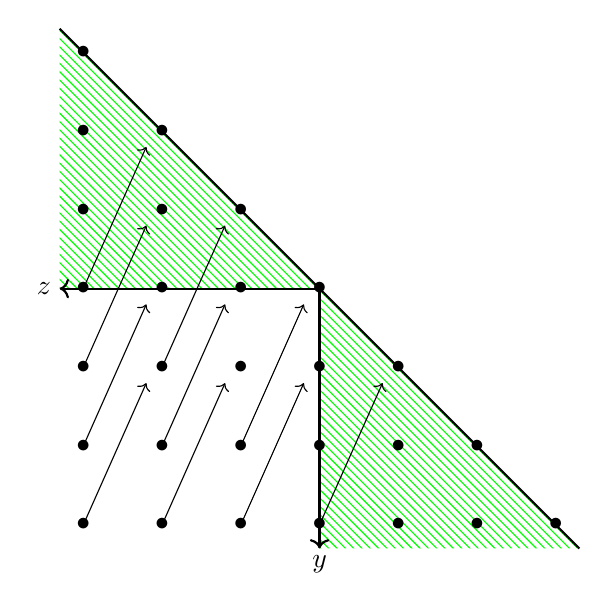
\begin{tikzpicture}
%    \foreach\ang in {60,120,...,360}{
%     \draw[->,blue!80!black,dotted] (0,0) -- (\ang:3cm);
%    }
%    \foreach\ang in {60,180, 300}{
%     \draw[->,black!80!black] (0,0) -- (\ang:1cm);
%    }
    \fill[pattern=north west lines, pattern color=green]    (0,0) -- (-3.3,0) -- (-3.3,3.3) -- (0,0) -- (0,-3.3) -- (3.3, -3.3) -- (0,0);
    \draw[->,black!80!black,thick] (0,0) -- (0,-3.3);
    \draw[->,black!80!black,thick] (0,0) -- (-3.3,0);
        \draw[-,black!80!black,thick] (-3.3,3.3) -- (3.3,-3.3);
    \node at (0,0) {$\bullet$};
    \node at (0,-1) {$\bullet$};
    \node at (0,-2) {$\bullet$};
    \node at (0,-3) {$\bullet$};
    \node at (1,-1) {$\bullet$};
    \node at (1,-2) {$\bullet$};
    \node at (1,-3) {$\bullet$};
    \node at (2,-2) {$\bullet$};
    \node at (2,-3) {$\bullet$};
    \node at (3,-3) {$\bullet$};
    \node at (-1,1) {$\bullet$};
    \node at (-1,0) {$\bullet$};
    \node at (-1,-1) {$\bullet$};
    \node at (-1,-2) {$\bullet$};
    \node at (-1,-3) {$\bullet$};
    \node at (-2,2) {$\bullet$};
    \node at (-2,1) {$\bullet$};
    \node at (-2,0) {$\bullet$};
    \node at (-2,-1) {$\bullet$};
    \node at (-2,-2) {$\bullet$};
    \node at (-2,-3) {$\bullet$};
    \node at (-3,3) {$\bullet$};
    \node at (-3,2) {$\bullet$};
    \node at (-3,1) {$\bullet$};
    \node at (-3,0) {$\bullet$};
    \node at (-3,-1) {$\bullet$};
    \node at (-3,-2) {$\bullet$};
    \node at (-3,-3) {$\bullet$};
    
    \node at (0,-3.5) {$y$};
    \node at (-3.5,0) {$z$};
    
    \draw[->,black!80!black] (-1,-2) -- (-.2,-.2);
    \draw[->,black!80!black] (-2,-2) -- (-1.2,-.2);
    \draw[->,black!80!black] (-3,-2) -- (-2.2,-.2);

    \draw[->,black!80!black] (-3,-3) -- (-2.2,-1.2);
    \draw[->,black!80!black] (-2,-3) -- (-1.2,-1.2);
    \draw[->,black!80!black] (-1,-3) -- (-0.2,-1.2);
    \draw[->,black!80!black] (0,-3) -- (0.8,-1.2);
    
    
    \draw[->,black!80!black] (-3,-1) -- (-2.2,0.8);
    \draw[->,black!80!black] (-2,-1) -- (-1.2,0.8);

    
    \draw[->,black!80!black] (-3,0) -- (-2.2,1.8);
  \end{tikzpicture}
\end{center}
where the shaded green (including boundaries) indicates the image of $k[x/z,y/z]$ and $k[x/y, z/y]$ in $k[x/z,x/y,z/y,y/z]$ and the arrows indicate reductions.  In particular, we see that the monomial $x^2/yz$ cannot be reduced, and therefore is the generator for $H^1$.

%In particular, this implies that $f$ is not flat, since the Euler characteristic is also drops since $h^0(X_t, \OO_{X_t}) = 1$ for all fibers.
\end{exmp}


\begin{exmp}[Degeneration to a node; Legrende family]
One can run the above example, with a little bit more work, for the degeneration of elliptic curves to a nodal rational curve given by the equation
$$y^2 = x(x+z)(x-zt).$$.  
%Here, the intuition is that the topological Euler characteristic for a nodal rational curve is $1$ (i.e. $\chi(S^1) - 1$ for the two points that get identified).  \todo{???}

%First, note that generically, we have $h^1(X_\xi, \mathcal{F}|_{X_\xi}) = 1$ by Riemann-Roch.  We claim that $h^1(X_0, \mathcal{F}|_{X_0}) = 0$.  Let us investigate what happens in this example.  Note that the basic opens obtained by setting $y = 1$ and $z = 1$ cover $X_0 \subset \PP^2$.  We wish to investigate the surjectivity of the map
%$$\frac{k[x/z, y/z]}{(y/z)^2 = (x/z)^2(x/z + 1)} \bigoplus \frac{k[x/y, z/y]}{1 = (x/y)^2(x/y+z/y)} \rightarrow \frac{k[x/z,x/y,z/y, y/z]}{(y/z)^2 = (x/z)^2(x/z + 1), 1 = (x/y)^2(x/y+z/y)}.$$
%The game is as follows.  Except for $(x/z) \cdot (y/z)$, the product of any two generators on the right-hand side is in the image of the map.  Thus we wish to investigate monomials of the form $x^{n+m}/y^n z^m$ where $n,m>0$.  We will use the equations on the right-hand side to make some reductions.  The first equation multiplied by $(z/y)^2$ tells us that
%$$\frac{x^3}{y^2 z} = 1 - \frac{x^2}{y^2}$$
%and so we can rewrite any monomial as a sum of monomials in the image and monomials $x^{1+m}/yz^m$.  Now, take the second equation and multiply it by $y/z$ to get
%$$\frac{y}{z} = \frac{x^3}{yz^2} + \frac{x^2}{yz}.$$
\end{exmp}

\newpage



\newpage





\section{Flatness as a notion of good behavior in families}

Slogan: lots of things very nicely in flat families, e.g. cohomology, dimension, Euler characteristic (and everything derived from Euler characteristic).


\subsection{Definition of flat and faithfully flat}

Recall that an $R$-module $M$ is \emph{flat} if $M \otimes_R -$ is left-exact.

\begin{exmp}
Projective $R$-modules are flat.  Localizations $S^{-1}R$ are not projective, but still flat.  We also have a partial converse: a flat finitely related module $M$ is projective.
\end{exmp}


\begin{prop}[On stalks]
An $R$-module $M$ is flat if and only if $M_{\mf{p}}$ is flat over $R_{\mf{p}}$ for all $\mf{p}$.
\end{prop}
\begin{proof}
The forward direct follows by transitivity of tensor product, and the fact that localizations are flat.  For the backwards direction, consider an injective morphism $N \rightarrow P$ and let $K = \ker(N \otimes_R M \rightarrow P \otimes_R M)$.  We want to show that $K = 0$.  Since localization is exact and commutes with tensor products, $K_{\mf{p}} = \ker(N_{\mf{p}} \otimes_{R_{\mf{p}}} M_{\mf{p}} \rightarrow P_{\mf{p}} \otimes_{R_{\mf{p}}} M_{\mf{p}})$, so $K_{\mf{p}} = 0$ for every prime, so $K = 0$.
\end{proof}


\begin{prop}
A finitely presented flat $R$-module is projective.
\end{prop}
\begin{proof}
We can assume $R$ is a local ring, i.e. check on stalks.  Use Nakayama to choose a presentation
$$0 \rightarrow K \rightarrow R^n \rightarrow M \rightarrow 0$$
where $n$ is the number of minimal generators of $M$ and $K$ is finitely generated (which we can guarantee using finite presentation of $M$).  We can tensor with $R/\mf{m}$, and since $\Tor^1_R(M, -) = 0$, the sequence is still exact, thus $K/\mf{m}K = 0$, therefore $K = 0$ by Nakayama.
\end{proof}

\begin{defn}
Let $f: X \rightarrow Y$ be a morphism of schemes, and $\mathcal{F}$ an $\OO_X$-module.  We say that $\mathcal{F}$ is \emph{flat over $Y$ at $x \in X$} if the stalk $\mathcal{F}_x$ is flat as an $\OO_{Y, y}$-module (where $y=f(x)$).  If $\mathcal{F}$ is flat over $Y$ for every $x \in X$ then we say that $\mathcal{F}$ is \emph{flat over $Y$}.  If $\OO_X$ is flat over $Y$ then we say \emph{$f$ is flat} or \emph{$X$ is flat over $Y$}.
\end{defn}

\begin{exmp}
Consider $\Spec k[t][x,y]/xy-t \rightarrow \Spec k[t]$.  This map is flat.
\end{exmp}

\begin{exmp}
Consider $\Spec k[t][x,y]/y^3 - (x^3 + x^2 + tx) \rightarrow \Spec k[t]$.  This map is flat.  It is a smooth curve generically and singular when $t=0, 1/4$.
\end{exmp}



Also useful will be the following.  We will soon see it geometrically corresponds to a flat surjective morphism.
\begin{defn}
We say an $R$-module $M$ is \emph{faithfully flat} if a sequence 
$$0 \rightarrow N' \rightarrow N \rightarrow N'' \rightarrow 0$$
is exact if and only if
$$0 \rightarrow N' \otimes_R M \rightarrow N \otimes_R M \rightarrow N'' \otimes_R M \rightarrow 0$$
is exact.  We say a map of schemes $f: X \rightarrow Y$ is \emph{faithfully flat} if it is flat and surjective on points.
\end{defn}

The following characterization is often useful.  Note that an exact functor of abelian categories $F$ is faithful if and only if $F(X) = 0$ implies $X = 0$, so this can serve as justification of the terminology.
\begin{lemma}
A flat $R$-module $M$ is faithfully flat if and only if $M \otimes_R N = 0$ implies that $N = 0$. 
\end{lemma}
\begin{proof}
Suppose $M$ is faithfully flat.  Consider the sequence 
$$0 \rightarrow N \rightarrow 0$$
as well as the sequence after applying $- \otimes_R M$.  Exactness means being zero, so we find that $N = 0$ if and only if $N \otimes_R M = 0$.  Conversely, let $N' \rightarrow N \rightarrow N''$ be a sequence which is exact after applying $- \otimes_R M$, i.e. middle homology $H(N)$ is zero.  By flatness of $M$, $H(N) \otimes_R M = H(N \otimes_R M) = 0$, so $H(N) = 0$, i.e. the original sequence was exact.
\end{proof}

\begin{exmp}
Let $M$ be $R[1/f]$ where $f$ is not a unit.  Then, $M$ is not faithfully flat, since $M \otimes_R R/f = 0$.
\end{exmp}


\begin{prop}
A map of affine schemes if faithfully flat if and only if the corresponding map on rings is faithfully flat.
\end{prop}
\begin{proof}
Take $f: X = \Spec(A) \rightarrow Y = \Spec(B)$.  Suppose $B \rightarrow A$ is faithfully flat, and let $y \in Y$ be a point downstairs.  The fiber $f^{-1}(y) = A \otimes_B \kappa(y)$ is nonzero if and only if $\kappa(y)$ is nonzero by the above lemma.  

Conversely, we will show that a flat map $f$ is surjective on points if and only if it is surjective on closed points.  Suppose that $f$ is surjective on closed points.  Let $N$ be a $B$-module, choose a cyclic $B$-submodule of $N$ isomorphic to $B/I$, and choose $\mf{m}$ containing $I$.  We have a diagram
$$\begin{tikzcd}
B/I \arrow[r, hook] \arrow[d, two heads] & N \\
B/\mf{m}
\end{tikzcd}$$
Tensoring $- \otimes_B A$, and using flatness so that injections and surjections are preserved, and the fact that $B/\mf{m} \otimes_B A$ is nonzero due to surjectivity on points, we find that $N$ is nonzero.
\end{proof}

In the above we proved the following.
\begin{prop}
A map of schemes $f: X \rightarrow Y$ is faithfully flat if and only if it is surjective on closed points.
\end{prop}


\subsection{Flat limits}

Remember that an associated prime of a ring $R$ is a prime $\mf{p}$ which is the annihilator of some $r \in R$.  Note that $r$ is not in any associated prime if and only if $r$ is a non-zerodivisor.
\begin{prop}
Let $f: X \rightarrow Y$ be a flat morphism of locally Noetherian schemes.  Then, $f$ sends associated points to associated points.
\end{prop}
\begin{proof}
Let $x \in X$ be an associated point, and $y = f(x)$.  We can check on local rings, i.e. let $f^\sharp: (A, \mf{p}_y) \rightarrow (B, \mf{p}_x)$ be a map of Noetherian local rings.  If $\mf{p}_y$ is not an associated prime, then there is $a \in \mf{p}_y$ not in any associated prime by prime avoidance\footnote{Geometrically, prime avoidance says that for any collection of points $x_1, \dots, x_n$ of a scheme $X$ and any closed subscheme $Z$ not containing any of the points, then affine locally, there is a function $f$ vanishing on $Z$ but not vanishing on any of the points $x_i$ (i.e. there is a Cartier divisor vanishing on $Z$ but not on any $x_i$).} and therefore a non-zerodivisor, i.e. the multiplication by $a$ map $\mu_a$ is injective.  Since $B$ is flat over $A$, $\mu_a \otimes_A B = \mu_{f^\sharp(a)}$ is injective, i.e. $f^\sharp(a) \in \mf{p}_x$ is a non-zerodivisor, i.e. $\mf{p}_x$ cannot be an associated prime.
\end{proof}

\begin{exmp}
We can see that $\Spec k[x,y]/xy \rightarrow \Spec k[x]$ is not flat.  The blow up of a point in a plane is not flat since flatness is preserved by base change, and we can take the fiber over any line in the plane through that point.
\end{exmp}

\begin{cor}
Let $f: X \rightarrow Y$ be a morphism of schemes with $Y$ integral and regular, and $\dim(Y) = 1$.  Then, $f$ is flat if and only if every associated point of $X$ maps to the generic point of $Y$.  If $X$ is reduced, then every irreducible component of $X$ dominantes $Y$.
\end{cor}

%\begin{exmp}
%Let $f: \tilde{X} \rightarrow X$ be a normalization map of a curve.  Then, $f$ cannot be flat. Since $f$ is affine, flatness of $f$ is equivalence to flatness of $f_* \OO_{\tilde{X}}$, a coherent sheaf.  By flatness, it is locally free, and in particular a line bundle.  
%\end{exmp}


%This isn't quite what we promised yet, since the inclusion of a closed point is not flat.
%\begin{cor}
%In the set-up above, let $y \in Y$ be any point, $X_y = X \times_Y \Spec \kappa(y)$ the fiber, and $\mathcal{F}_y$ pullback of $\mathcal{F}$ to the fiber.  We abusively let $\kappa(y)$ denote the constant sheaf on $Y' = \overline{\{y\}}$.  Then, there are natural isomorphisms
%$$H^i(X_y, \mathcal{F}_y) \simeq H^i(X, \mathcal{F} \otimes \kappa(y)).$$
%\end{cor}
%\begin{proof}
%We can assume that $Y$ is affine, and let $X' = Y' \times_Y X$.  Note that $\Spec \kappa(y) \rightarrow Y$ factors through $Y'$.  
%\end{proof}


\begin{exmp}
The normalization of a node is not flat.
\end{exmp}

We can take ``flat limits'':
\begin{prop}
Let $Y$ be one-dimensional Noetherian scheme and $y \in Y$ a regular point, and $X$ a locally Noetherian scheme with a map $f: X \rightarrow Y$.  Let $Y* := Y - \{y\}$.  Given a closed subscheme $Z \subset f^{-1}(Y*)$ flat over $Y*$, the scheme theoretic closure $\overline{Z}$ is flat over $Y$.  Furthermore, it is the unique extension which is flat over $Y$.
\end{prop}

\begin{defn}
We call $\overline{Z}_y$ the \emph{flat limit} of $Z$.
\end{defn}

\begin{proof}
The associated points of $\overline{Z}$ are the associated points of $Z$, so $\overline{Z}$ is flat over $Y$ if $Z$ is flat over $Y*$.
\end{proof}

\begin{rmk}
What this says is that the Hilbert scheme is proper, by taking $X = \PP^n_Y$.
\end{rmk}

\begin{exmp}
The limit can be empty if $f$ is not proper.  For example, take $Y = \Spec k[t]$, and $X = \Spec k[t, x]/xt-1$.  The map is an isomorphism away from $t=0$.
\end{exmp}

\begin{exmp}
Take the limit of two skew axes in $\mathbb{A}^3$ which limit together (intersecting at a point).  Claim: the limit is not reduced and has an embedded point.  We take the family over $t$ in variables $x,y,z$ given by the equations $y=z=0$ and $x=z-t=0$.  At $t = 0$, it is defined by the ideal $(y,z)(x,z)$ which is not reduced.
\end{exmp}

%\begin{exmp}[Asymptotics]
%Let $X \subset \PP^n_k$ be a closed subscheme, and assume that $[0:\cdots:0:1] \not\in X$.  We consider a constant family $X \times \G_m \rightarrow \G_m$ with an embedding $X \times \G_m \subset \PP^n_k \times \G_m$ given by $([x_0:\cdots:x_n], t) \mapsto [x_0:\cdots:x_{n-1}:tx_n]$.  The limit has the same underlying space as the projection away from $[0:\cdots:0:1]$, but may be a different scheme structure that ``remembers'' that it came from a family.
%
% \todo{???} hartshorne 9.8.4 and vakil 24.4.L and 24.4.14
%\end{exmp}
%




\subsection{Dimension is constant in flat families}

We will first review two commutative algebra notions: going up and going down.  We will translate the commutative algebra language into a more geometric language.

\begin{defn}
Let $f: X = \Spec(A) \rightarrow Y = \Spec(B)$ be map of affine schemes.  We say a prime $x = \mf{p} \subset A$ \emph{lies over} $y = \mf{q} \subset B$ if $\phi^{-1}(\mf{p}) = \mf{q}$.  Geometrically, this just means that $f(x) = y$.

A map of rings has the \emph{going up property} if for any \underline{increasing}\footnote{Going ``up'' refers to the chain of prime ideals, not to the fact that we are ''going up'' in the lifting.} chain of prime ideals $\mf{p}_1 \subset \cdots \subset \mf{p}_n \subset B$ and corresponding chain $\mf{q}_1 \subset \cdots \subset \mf{q}_m \subset A$ with $m<n$ and $\phi^{-1}(\mf{p}_i) = \mf{q}_i$, one can complete the chain of prime ideals in $A$ to lie over the chain in $B$.

Geometrically, primes correspond to points.  If $x,x' \in X$ such that $\mf{p}_x \subset \mf{p}_{x'}$, we say that $x'$ is a \emph{specialization} of $x$, or $x'$ is a \emph{generalization} of $x$.  We say $f$ has the \emph{going up property} or the \emph{specialization lifting property} if for $x \in X$ and $y = f(x)$, and any specialization $y'$ of $y$, there is a lift $x'$ such that $f(x') = y'$.
\end{defn}



\begin{exmp}
The map $\mathbb{A}^2_k \rightarrow \mathbb{A}^1_k$ does not have the lying over property.  To see this, take $y_1$ to be the generic point of $\AAA^1$, and $y_2 = \{0\}$.  Take $x_1$ to be the generic point of the closed subscheme defined by $xy-1$.  There is no point of this closed subscheme over $0$, so the sequence cannot be completed.
\end{exmp}

%We recall the following without proof.
%\begin{thm}[Lying over theorem]
%Let $\phi: B \rightarrow A$ be an integral extension (i.e. injective).  Then $f: \Spec(A) \rightarrow \Spec(B)$ is surjective.
%\end{thm}

We state the following without proof for completeness.
\begin{thm}[Going up theorem]
Let $\phi: B \rightarrow A$ be integral\footnote{A map of rings $\phi: B \rightarrow A$ is \emph{integral} if every $a \in A$ satisfies a monic polynomial with coefficients in $\phi(B)$.}.  Then $\phi$ has the going up property.
\end{thm}

We are, instead, interested in the going down property, which is the analogous property for a \underline{decreasing} chain of ideals.
\begin{defn}
We say $f: X \rightarrow Y$ has the \emph{going down property} or the \emph{generalization lifting property} if for $x \in X$ and $y = f(x)$, and any generalization $y'$ of $y$, there is a lift $x'$ such that $f(x') = y'$.
\end{defn}

\begin{exmp}
The inclusion of a point $\pt \rightarrow \AAA^1$ does not satisfy the going down property.
\end{exmp}

\begin{thm}[Going down theorem for flat morphisms]
Flat morphisms have the going down property.
\end{thm}
\begin{proof}
Take $f: X = \Spec(A) \rightarrow Y = \Spec(B)$.  Let $y, y' \in Y$ such that $\mf{p}_{y'} \subset \mf{p}_{y}$ (i.e. $y'$ is a generalization of $y$), and let $x \in X$ such $f(x) = y$.  We claim that the localization of $f$ at $y$ is \emph{faithfully} flat; it is flat since localizations of flat maps are flat, and it is faithful since it is surjective on the only closed point (this uses the fact that one can lift $y$).  Thus, $f$ is surjective on points, and in particular one can lift $y'$.
\end{proof}



This allows us to prove the following.
\begin{thm}
Let $f: X \rightarrow Y$ be a flat morphism of locally Noetherian schemes.  Let $x \in X$ and $y = f(x)$.  Then
$$\codim_X(x) = \codim_Y(y) + \codim_{f^{-1}(y)}(x).$$
In particular, if $X$ and $Y$ are irreducible, then the fibers of $f$ have dimension $\dim(X) - \dim(Y)$.
\end{thm}
\begin{proof}
We proved earlier that
$$\codim_X(x) \leq \codim_Y(y) + \codim_{f^{-1}(y)}(x).$$
For the $\geq$, we use the going down theorem.  The codimension of $y$ is the maximal length of a chain of increasingly general ideals contained in $y$.  By the going down theorem, this can be lifted to $X$.  The inverse image of any chain of ideals containing $\mf{p}_x$ in $f^{-1}(y)$ gives a chain in $X$ containing $\mf{p}_y$, and the concatenation of these two chains gives a (possibly not maximal) chain in $X$ which gives the desired inequality.
\end{proof}


\subsection{Euler characteristic is constant in flat families}


The the following theorem we will use the following two facts.
\begin{lemma}
Let $M_0 \rightarrow \cdots \rightarrow M_n$ be an exact sequence of $R$-modules.  Then, (1) if each $M_i$ is flat, then tensoring $- \otimes_R N$ with any $N$ is exact, and (2) if $M_0 = 0$ and the $M_i$ are flat for $i \ne 1$, then $M_1$ is also flat.
\end{lemma}
\begin{proof}
There are two more or less equivalent proofs: one using long exact sequences and induction, and one using spectral sequences.  Let us sketch the latter.  Write out the sequence in the proposition as the $0$th ``row'' of a double complex.  Let $N$ be some $R$-module.  Resolve $N$ via a free resolution in each column (i.e. each column is tensored with $F_0 \rightarrow F_1 \rightarrow \cdots$).  

For (1), if we take the spectral sequence by taking cohomology with respect to the rows first, everything dies since free modules are flat and therefore preserves exactness.  If we take the spectral sequence by taking cohomology with respect to the columns first, we get back the original sequence tensored with $N$.  Since the spectral sequence converges to $0$, this sequence must be exact.

For (2), we take cohomology with respect to the columns first; the columns are $\Tor_j(M_i, N)$ which vanishes when $i \ne 1$, and the sequence must degenerate here since everything is in a single column.  If we took cohomology with respect to the rows instead, we find that everything dies since free modules are flat, i.e. all the higher Tor vanish, i.e. $M_1$ is also flat. 
\end{proof}

\begin{thm}
Let $f: X \rightarrow Y$ be a projective morphism of locally Noetherian schemes, and $\mathcal{F} \in \Coh(X)$ is flat over $Y$.  Then, $\chi(X_y, \mathcal{F}_y)$ is a locally constant function of $y \in Y$.
\end{thm}
\begin{proof}
We may assume $Y = \Spec B$ is affine.  We may assume that $X = \PP^n_B$ is projective space by pushing forward $\mathcal{F}$.  Take $r$ large enough so that $\mathcal{F}(r)$ has vanishing higher cohomology.

Let
$$0 \rightarrow f_* \mathcal{F}(r) \rightarrow \rightarrow \mathcal{C}^0 \rightarrow \cdots \rightarrow \mathcal{C}^n \rightarrow 0$$
be the augmented Cech complex.  The terms $\mathcal{C}^i$ are flat, since flatness is closed under restriction, and pushforward along maps of affines.  Thus, the term $f_* \mathcal{F}(r)$ is flat as well by the above lemma.  It is also coherent, which means it is locally free of finite rank.

Since the augmented Cech complex consists of flat modules, it is still exact after tensoring with $\kappa(y)$ by the lemma above, and so the alternating sum of the fibers at $y$ in the Cech complex is just
$$\chi(X_y, \mathcal{F}_y(r)) = \dim_{\kappa(y)}(f_*\mathcal{F}(r) \otimes_B \kappa(y))$$
by exactness of the complex.  Thus $\chi(X_y, \mathcal{F}_y(r))$ is the rank of $f_* \mathcal{F}(r)$ which is locally constant on $Y$.  In particular, the Hilbert polynomial (which we know is a polynomial, not just a function) $p_{\mathcal{F}_y}(t)$ locally constant for $t \gg 0$, meaning it is locally constant for all $t$.
\end{proof}

\begin{cor}
In the above setup, the Hilbert polynomial, arithmetic genus, fiber degree and fiber dimension are locally constant in $Y$.
\end{cor}
\begin{proof}
The Hilbert polynomial and arithmetic genus are defined in terms of the Euler characteristic.  The fiber degree is defined in terms of the Hilbert polynomial.  The fiber dimension is the degree of the Hilbert polynomial.
\end{proof}

\newpage


\section{Base change and upper semicontinuity}


We begin with the ``tautological'' base change.
\begin{prop}[Flat base change]
Let $f: X \rightarrow Y$ be a quasi-compact quasi-separated morphism.  Consider the Cartesian square
$$\begin{tikzcd}
X' \arrow[r, "g'"] \arrow[d, "f'"] & X \arrow[d, "f"] \\
Y' \arrow[r, "g"] & Y.
\end{tikzcd}$$
For $\mathcal{F} \in \QCoh(X)$, there is a natural morphism of functors 
$$\psi: g^* R^i f_* \rightarrow R^if'_*, g'^*$$
which is an isomorphism if  $g: Y' \rightarrow Y$ is flat.
\end{prop}
\begin{proof}
We reduce to the case when $Y', Y$ are affine.  By the sheaf property it suffices to compute at small open neighborhoods at every point $y' \in Y'$.  Choose an open affine $\Spec B \subset Y$ containing $y = g(y')$ and an open affine $\Spec A \subset g^{-1}(\Spec B)  \subset Y'$.  We will simply take $Y = \Spec B$ and $Y' = \Spec A$.


We want to define a map
$$H^i(X, \mathcal{F}) \otimes_B A \rightarrow H^i(X', g'^* \mathcal{F}).$$
We can compute $H^i$ using a finite Cech complex since $f$ (and therefore $X$, now that $Y$ is affine) is quasi-separated and quasi-compact.  Take $U$ to be a finite open affine cover of $X$ and $U' := g'^{-1}U_i = U_i \times_Y Y'$ the corresponding finite open affine\footnote{Since now $Y, Y'$ are affine.} cover of $X'$.  Since the Cech complexes are finite, products are sums, which commute with tensor products, and we have a canonical identification of Cech complexes (more or less by definition of fiber product):
$$C^\bullet(U',g'^* \mathcal{F}) =  C^\bullet(U, \mathcal{F}) \otimes_B A.$$
Thus the desired map should take the form
$$H^i(C^\bullet(U, \mathcal{F})) \otimes_B A \rightarrow H^i(C^\bullet(U, \mathcal{F}) \otimes_B A)).$$
The universal property of extension of scalars gives the map via the map $H^i(C^\bullet(U, \mathcal{F})) \rightarrow H^i(C^\bullet(U, \mathcal{F}) \otimes_B A))$ coming from the underlying map on complexes.  If $A$ is flat over $B$, then $- \otimes_B A$ is exact so the map is an isomorphism.
\end{proof}

\begin{rmk}
The above is true without the flatness assumption by replacing $g^*, g'^*$ with $Lg^*, Lg'^*$ by essentially the same argument.  That is, there is a natural quasi-equivalence of functors on $D^-(\QCoh(Y'))$:
$$Lg^* Rf_* \rightarrow Rf'_* Lg'^*.$$
When $g$ is flat, $g'$ is also flat and we have $Lg^* = g^*$ and $Lg'^* = g'^*$, and also $g^*$ commutes with cohomology, so $H^i(g^* Rf_*) = g^* R^i f_*$.  However, we are still interested in the morphism $\psi$ in the non-flat case, which does not really make sense in the derived category.
\end{rmk}

\begin{defn}
We call the morphism $\psi$ constructed above the \emph{base change morphism}.  We will sometimes write $\psi_{Y'}$ to indicate what we are base-changing to.  We are interested in studying when it is an equivalence, in particular when $Y = \Spec \kappa(y)$ for $y \in Y$, i.e. ``fiber of cohomology is cohomology of fiber.''
\end{defn}

The above tells us that ``fiber of cohomology is cohomology of the fiber'' at the generic point.
\begin{cor}
Let $f: X \rightarrow Y$ be a separated morphism of finite type, and $X, Y$ Noetherian schemes with $Y$ integral.  Let $\xi$ be the generic point of $Y$.  Then,
$$(Rf_* \mathcal{F})_\xi \simeq Rf'_*(\mathcal{F}|_{X_\xi}).$$
\end{cor}

\subsection{Upper semicontinuity}

Our goal is to prove the following theorem.  Recall that any map out of a locally Noetherian scheme is quasi-separated, so we may replace the quasi-separated condition with $X$ being locally Noetherian.
\begin{thm}[Upper semicontinuity]
Let $f: X \rightarrow Y$ be a proper quasi-separated morphism with $Y$ locally Noetherian, and $\mathcal{F} \in \Coh(X)$ flat over $Y$.  Then, the function
$$y \mapsto \dim_{\kappa(y)}(H^i(X_y, \mathcal{F}|_{X_y}))$$
is upper semicontinuous\footnote{This means that the inverse image of $(-\infty, a]$ must be open, i.e. cohomology groups can ``jump.''}  for every $i$.
\end{thm}

\begin{exmp}[Counterexamples]
This can fail without the hypotheses.  Take any open embedding ($f$ fails to be proper), or take $f$ to be the identity and push forward along a basic open embedding ($\mathcal{F}$ is not coherent).  Without the flatness assumption, take $f: X = \mathrm{Bl}_{(0,0)}(\mathbb{A}^2) \rightarrow Y = \mathbb{A}^2$ to be the blow-up of of the plane at a point.  There is a closed embedding $i: X \rightarrow \mathbb{P}^1 \times \mathbb{A}^2$; take $\mathcal{F} = i^* (\OO_{\mathbb{P}^1}(-1) \boxtimes \OO_{\mathbb{A}^1})$.  Then, for $y \ne (0,0)$, $X_y = \pt$ is a point so $h^0 = 1$, while $X_{(0,0)} = \mathbb{P}^1$ and $\mathcal{F}|_{X_{(0,0)}} = \OO(-1)$, so $h^0 = 0$.
\end{exmp}



\begin{exmp}[Example of jumping cohomology]
Take the projection $f: E \times E \rightarrow E$ where $E$ is an elliptic curve.  Fix a point $p_0 \in E$ and let $\mathcal{L}$ be a line bundle which is $\LL(p - p_0)$ over $p \in E$.  Then, $Rf_* \mathcal{L} = 0$ away from $p_0$ and is $R^0f_* \mathcal{L} = R^1 f_* \mathcal{L} = k$ at $p_0$.
\end{exmp}

Our main tool is the following result of Mumford, which essentially gives a procedure for replacing right-bounded complexes with coherent cohomology which may have very complicated terms with right-bounded finitely rank free complexes.
\begin{lemma}[Key lemma]
Let $f: X \rightarrow Y  = \Spec B$ be a proper quasi-separated morphism where $B$ is Noetherian, and $\mathcal{F} \in \Coh(X)$ flat over $Y$.  Let $g: Y = \Spec A \rightarrow Y$ be a map of affine schemes.  Then there is a complex (the ``Grothendieck complex'')
$$\cdots \rightarrow K^{-1} \rightarrow K^0 \rightarrow \cdots \rightarrow K^n \rightarrow 0$$
of finitely generated free $B$-modules and an isomorphism of functors
$$H^i(X \times_Y Y', g'^* \mathcal{F}) \simeq H^i(K^\bullet \otimes_B A)$$
\end{lemma}
\begin{proof}
Fix a finite open cover $U$ of $X$.  Let $\mathcal{C}^\bullet(U_i, \mathcal{F})$ denote the (alternating, i.e. ``reduced'') Cech complex.  Then $f_* \mathcal{C}^\bullet(U_i, \mathcal{F}))$ is a complex whose terms which has bounded and finitely generated cohomology, but whose terms are flat and not finitely generated.  We will decsribe a procedure for producing a complex $K^\bullet$ which is only right-bounded with finite-rank free terms, and a quasi-isomorphism
$$K^\bullet \rightarrow f_* \mathcal{C}^\bullet(U_i, \mathcal{F})).$$
Let us prove the lemma assuming this.  Note that $U' := g^{-1}(U)$ is an open affine cover of $X \times_Y Y'$, so we can use it to compute the Cech complex, and in particular we find that
$$\begin{tikzcd}
f'_* \mathcal{C}^\bullet(U', g'^*\mathcal{F}) \arrow[r, "\cong"] & f_* \mathcal{C}^\bullet(U, \mathcal{F}) \otimes_B A & \arrow[l, "\simeq"'] K^\bullet \otimes_B A\end{tikzcd}$$
where the last isomorphism uses the fact\footnote{Quick proof: the mapping cone of flat complexes is flat, and a map is a quasi-isomorphism if and only if the mapping cone is acyclic.  Thus, it suffices to show that $- \otimes_B A$ applied to the mapping cone is acyclic.  This follows from the usual Tor argument for complexes with flat terms.} that $- \otimes_B A$ preserves quasi-isomorphisms between complexes of right-bounded flat $B$-modules (even though $A$ is not flat over $B$).  This is where we use the fact that $\mathcal{F}$ is flat; so that $f_* C^\bullet(U, \mathcal{F})$ consists of flat $B$-modules.




Now we construct $K^\bullet$.  More generally, let $M^\bullet$ be a right-bounded complex of $B$-modules with coherent cohomology.  We will describe the inductive step of producing this complex.  Suppose we are at the stage
$$\begin{tikzcd}
& & K^{i+1} \arrow[r] \arrow[d] & K^{i+2} \arrow[r] \arrow[d] & \cdots \\
\cdots \arrow[r] & M^i \arrow[r] & M^{i+1} \arrow[r] &M^{i+2} \arrow[r]&\cdots
\end{tikzcd}$$
where the map of complexes is an isomorphism on $H^{\geq i+2}$ and surjective on $H^{i+1}$.  We produce generators for $K^i$ corresponding to
\begin{enumerate}[(1)]
\item generators for $\ker(K^{i+1} \rightarrow H^{i+1}(M^\bullet)$, which will kill $\ker(H^{i+1}(K^\bullet) \rightarrow H^{i+1}(M^\bullet))$,
\item generators for $H^i(M^\bullet)$ which will produce a surjective map on $H^i$.
\end{enumerate}
Build $K^i$ as above and map as described above and describe how to map the generators to $M^i$ and $K^{i+1}$ to get a map of complexes.  Note we use the fact that $B$ is Noetherian to get finitely many generators at each stage.
\end{proof}




\begin{proof}[Proof of upper semicontinuity]
We may assume $Y$ is affine.  Take $y \in Y$, $K^\bullet$ as in the above lemma, and $Y = \Spec \kappa(y)$.  Then,
$$\dim_{\kappa(y)}(H^i(X_y, \mathcal{F}|_{X_y}) = \dim_{\kappa(y)}(H^i(K^\bullet \otimes_B \kappa(y))).$$
By rank nullity, this is the rank of the $i$th term in $K^\bullet$ minus the ranks of adjacent differentials in the complex $K^\bullet \otimes_B \kappa(y)$, we want that ranks of matrices are lower semicontinuous, which is true since the locus on $\Spec(B)$ where a given matrix has rank $\leq n$ is cut out by setting all $n \times n$ minors equal to $0$.
\end{proof}

\begin{rmk}
This can be used to extend the fact that Euler characteristic is locally constant in flat families to the proper case, since Euler characteristic is equal to the alternating sum of ranks which is locally constant.
\end{rmk}

\subsection{Grauert's theroem and base change theorem}


\begin{rmk}[Relationship to base change]
Base change holds for $B \rightarrow A$ if and only if $$H^i(K^\bullet \otimes_B A) = H^i(K^\bullet) \otimes_B A$$
where $K^\bullet$ is the complex obtained in the key lemma.
\end{rmk}

We will use the following technical lemma.
\begin{prop}
Let $X$ be a reduced scheme and $\mathcal{F}$ a constant rank finite type sheaf on $X$.  Then, $\mathcal{F}$ is locally free.
\end{prop}
\begin{proof}
Let $r$ be the rank of $\mathcal{F}$ (which is constant).  Let $x \in X$ be any point; we will show $\mathcal{F}_x$ is free over $\OO_{X, x}$.  Use Nakayama to lift generators of the $r$-dimensional vector space $\mathcal{F} \otimes_{\OO_X} \kappa(x)$ to $\mathcal{F}_x$.  By ``deleting denominators'' we can find an open affine $U = \Spec(A) \subset X$, lift the generators to $\mathcal{F}(U)$, and define a map $A^{\oplus n} \rightarrow \mathcal{F}(U)$.  Suppose $(a_1, \ldots, a_n)$ is in the kernel of this map and reorder so that $a_1 \ne 0$.  Since $A$ is reduced, the nilradical of $A$ is zero, and in particular there is a prime $\mf{p}_y \in U$ which does not contain $a_1 \ne 0$.  Then, $a_1$ is invertible in $R_{\mf{p}_{y}}$, so $\mathcal{F}_y$ can be written in terms of $n-1$ generators, contradicting constant rank.
\end{proof}

\begin{exmp}
The above can fail without the reducedness hypothesis, e.g. $X = \Spec k[x]/x^2$ and $\mathcal{F} = k[x]/x$.
\end{exmp}
%
%We will use the following homological algebra lemma.
%\begin{lemma}
%Let $\mathcal{M}^\bullet$ be a complex of $B$-modules, and let $N$ be a $B$-module with free resolution $F^\bullet \rightarrow N$.  Let $\tau^{\leq i}$ denote the soft truncation.  Then, $(\tau^{\leq i} M^\bullet) \otimes_B F^\bullet \rightarrow M^\bullet \otimes_B F^\bullet$ induces an isomorphism on $H^i$.
%\end{lemma}
%\begin{proof}
%Write down the double complex and run the spectral sequence.
%\end{proof}


The following gives us a condition for when the cohomology of fibers is isomorphic to fiber of cohomology.  
\begin{thm}[Grauert]
Let $f: X \rightarrow Y$ be a proper quasi-separated morphism with $Y$ reduced.  Let $\mathcal{F} \in \Coh(X)$ which is flat over $Y$.  Fix $i \in \Z$.  Assume that  $h^i(X_y, \mathcal{F}|_{X_y})$ is locally constant in $y \in Y$.  Then, $R^if_*\mathcal{F}$ is locally free and the base change morphism is an isomorphism for all $g: Y' \rightarrow Y$.
\end{thm}
\begin{proof}
We may assume both $Y = \Spec B$, $Y' = \Spec A$ are affine.  We may also assume that $h^i(X_y, \mathcal{F}|_{X_y})$ is constant on $Y$.  By the same argument as in the proof of upper semicontinuity, we have that the differentials adjacent to $K^i$ have constant rank:
$$\begin{tikzcd}
K^{i-1} \arrow[r, "d"] & K^i \arrow[r, "d'"] & K^{i+1} 
\end{tikzcd}$$
Thus the cokernels $W^i, W^{i+1}$ have constant rank (since cokernels commute with tensor products).  By the above Lemma, using reducedness, we have that the cokernels (of the adjacent differentials) are locally free.  Furthermore, we have the coboundaries $B^{i+1}$ are locally free via the short exact sequence:
$$0 \rightarrow B^{i+1} \rightarrow K^{i+1} \rightarrow W^{i+1} \rightarrow 0.$$
Then, by the short exact sequence
$$0 \rightarrow H^i(K^\bullet) \rightarrow W^i \rightarrow B^{i+1} \rightarrow 0$$
we have that $H^i(K^\bullet)$ is locally free.  To see that base change induces an isomorphism, note that applying $- \otimes_B A$ to the second short exact sequence implies that $H^i(K^\bullet) \otimes_B A \simeq H^i(K^\bullet \otimes_B A)$.
\end{proof}

\begin{rmk}
The converse is easy to verify: if $R^if_* \mathcal{F}$ is locally free and the base change morphism for $\kappa(y) \rightarrow Y$ is an isomorphism, then $h^i(X_y, \mathcal{F}|_{X_y})$ is locally constant.
\end{rmk}


We leave the proof of the following as an exercise, see Vakil 28.G-K.
\begin{thm}[Base change theorem]
Let $f: X \rightarrow Y$ be a proper morphism with $Y$ locally Noetherian.  Let $\mathcal{F} \in \Coh(X)$ which is flat over $Y$.  Fix $i \in \Z$.  Assume that the base change map is surjective for $\kappa(y) \rightarrow Y$.  Then: \\
\indent (i) There is an open neighborhood $U$ of $y$ such that for any $Y' \rightarrow Y$ factoring through $U$, the base change map is an isomorphism on $H^i$. \\
\indent (ii) The base change map for $i-1$th cohomology is surjective if and only if $(R^if_* \mathcal{F})_y$ is free.
\end{thm}

\begin{rmk}
Note that (ii) above means that we can continue ``inducting down'' the cohomology, and that surjectivity of the base change map for $i$ and $i-1$ implies that $h^i$ is constant in a neighborhood of $y$.
\end{rmk}

%\begin{proof}
%Assume that both $Y = \Spec B$ and $Y' = \Spec A$ are affine, where $B$ is Noetherian.  Recall the local criterion for flatness: if $(B, \mf{n}) \rightarrow (A, \mf{m})$ is a map of local rings and $M$ an $A$-module, then $M$ is flat over $B$ if and only if $\Tor_1^A(M, A/\mf{m}) = 0$.
%
%
%\end{proof}


\newpage


\section{Hilbert and Quot schemes}

\subsection{Definition, statements, and plan}

We first recall some notation.
\begin{defn}[Functor of points notation]
Let $X, T$ be schemes.  Then, $X(T) = \Hom_{\cat{Sch}}(T, X)$ are the \emph{$T$-points} of $X$.  Given $s \in X(T)$ and $p: X' \rightarrow X$, we write $s^*X' = X' \times_X T$ to be the pullback of $X'$ along $s$ and $s^* p: X' \times_X T \rightarrow T$ the pullback of $p$ along $s$.  If $\mathcal{F}$ is a sheaf on $X'$, we abusively use $s^* \mathcal{F}$ to denote the pullback to $s^*X'$.
\end{defn}

\begin{defn}
Let $F: \cat{Sch}^{op} \rightarrow \cat{Set}$ be a functor.
\begin{itemize}
\item A \emph{fine moduli space} for $F$ is a scheme $M$ and an isomorphism of functors $\phi: F \rightarrow \Hom_{\cat{Sch}}(-, M)$.  
\item A \emph{coarse moduli space} for $F$ is a scheme $M$ which is initial amongst schemes $X$ equpped with functors $F \rightarrow \Hom_{\cat{Sch}}(-, M)$, and such that $F(\Spec k) = M(k)$ for $k = \overline{k}$.
\end{itemize}
A fine moduli space is evidently also a coarse moduli space.
\end{defn}


\begin{rmk}
There is another equivalent way to say what it means to be a fine moduli space.  Note that the isomorphism $\phi$ determines a universal element $u \in F(M)$ corresponding to the identity map, universal in the sense that for every $x \in F(T)$ there is a unique $f: T \rightarrow M$ such that $f^*(u) = x$.
\end{rmk}

\begin{rmk}
The definition of moduli space can be tweaked:
\begin{itemize}
\item The category $\cat{Sch}$ can be replaced with a different category of schemes.  For example, we can work over a base shceme $S$ and take $\cat{Sch}_S$ the category of schemes over $S$.
\item We will simplify the exposition by making the following assumption: $\cat{Sch}_S$ is the category of \underline{locally Noetherian} schemes over the locally Noetherian scheme $S$.  Most statements will be true in greater generality.
\item The target category $\cat{Set}$ can be replaced with another category.  For example, replacing $\cat{Set}$ with $\cat{Grp}$ means that the moduli space is a \emph{group scheme}.  This is easy to check using Yoneda: if the functor-of-points of a representable functor induces group objects in sets, then it comes from a group object in schemes.
\end{itemize}
\end{rmk}

\begin{defn}[Hilbert functors]
Let $S$ be a Noetherian scheme, and $X$ a finite-type scheme over $S$ (for example, $X = \mathbb{P}^n_S$).  The \emph{Hilbert functor} associated to this data is the functor\footnote{It is a functor since properness and flatness is preserved by base change.} $H_{X/S}: \cat{Sch}_S^{op} \rightarrow \cat{Set}$ where, for $s \in S(T)$ we have
$$H_{X/S}(s) = \left\{i: Z \subset X \text{ closed subscheme} \mid s \circ i: Z \rightarrow T \text{ flat, proper} \right\}.$$
Note there are no automorphisms to quotient by.  The fine moduli space, if it exists, is the \emph{Hilbert scheme} and is denoted $\Hilb_{X/S}$.
\end{defn}

\begin{defn}[Quot functors]
In the set-up above, fix in addition $\mathcal{E} \in \Coh(X)$ (not necessarily flat).  The \emph{Quot functor} $Q_{\mathcal{E}/S}: \cat{Sch}_S^{op} \rightarrow \cat{Set}$ is given by\footnote{Note there is no need to consider equivalence classes under the first definition, but we often think in terms of the second.  In the case that $\mathcal{E} = \OO_X$, this is the difference between thinking in terms of an ideal sheaf versus the structure sheaf of the corresponding closed subscheme.}
$$Q_{\mathcal{E}/S}(s)  = \{ \mathcal{K} \subset s^* \mathcal{E} \mid s^*\mathcal{E}/\mathcal{K} \text{ flat and proper over } T\} = 
\left. \left\{ \begin{array}{l}  q: s^* \mathcal{E} \twoheadrightarrow \mathcal{F} \\ \mathcal{F} \in \Coh(s^* X) \end{array} \middle| \mathcal{F} \text{ flat and proper over } T  \right\}  \middle/ \sim  \right.$$
where by proper over $T$ we mean the scheme-theoretic support (equivalently the reduced set-theoretic support) is proper over $T$.  The fine moduli space, if it exists, is the \emph{Quot scheme}, denoted $\Quot_{\mathcal{E}/S}$.
\end{defn}

\begin{rmk}
The Hilbert functor is a special case of the Quot functor, where we take $\mathcal{E} = \OO_X$.  We will generally not discuss Hilbert functors from now on and subsume them as a special case of Quot functors.
\end{rmk}

%\begin{exmp}
%If $X = S$ and $\mathcal{E} \in \Coh(X)$ is flat (in particular, locally free), then $Q_{\mathcal{E}/S}$ is a \emph{Grassmannian functor}.  In particular, if $S = \Spec k$ for a field $k$, this is always the case.  We will explore this ``easy'' case in detail in the next section, and it will be an important step in proving the main representability theorem below.
%\end{exmp}

\begin{defn}[Hilbert polynomials in generality]
We can define the notion of a Hilbert polynomial for a non-projective scheme over a field $k$ (though we will only prove things in the projective case, so this isn't strictly necessary).  Let $X$ be a finite-type Noetherian scheme over a field $k$, and $\mathcal{L}$ a line bundle\footnote{The line bundle is almost always assumed to be very ample, but it does not have to be for the definition to make sense.} on $X$.  For $\mathcal{F} \in \Coh(X)$ whose \underline{support is proper} over $S$ we define
$$h^{\LL}_{\mathcal{F}}(t) = \chi(X, \mathcal{F} \otimes_{\OO_X} \mathcal{L}^{\otimes t}).$$
A priori, it is not clear that this is a polynomial (since we do not have the Hilbert syzygy theorem at our disposal).  This is due to ``Snapper's lemma.''
\end{defn}

\begin{defn}[Quot functor with a specified Hilbert polynomial]
In the set-up above, and letting $h \in \Q[t]$, we define by $Q^h_{\mathcal{E}/S}$ to be the subfunctor of $Q_{\mathcal{E}/S}$ define at $s \in S(T)$ to be the subset of sheaves $\mathcal{F} \in \Coh(s^*X)$ whose Hilbert polynomial at every scheme point $t \in T$ is $h(t)$.  Since the Hilbert polynomial is locally constant in flat families and $\mathcal{F}$ is flat over $T$, we have that $Q^h_{\mathcal{E}/S} \subset Q_{\mathcal{E}/S}$ is both a relative open and closed embedding.
\end{defn}

The following Grassmannian functor is an easy case of the above Quot functor where $X = S$.  We will construct its moduli space explicitly in the next section.
\begin{defn}
Fix a base scheme $S$.  Let $X = S$ and $\mathcal{E}$ a rank $n$ vector bundle on $S$.  Consider the constant (Hilbert) polynomial $h(t) = r$ where $r \in \Z^{\geq 0}$.  We define the \emph{Grassmannian functor} to be the Quot functor $Q_{\mathcal{E}/S}^h$, i.e. we are specifying that the quotient has rank $r$.  We sometimes write this $G_{\mathcal{E}/S}^r$ to emphasize that it is the Grassmannian.  If it is representable, we denote its representing scheme by $\Gr_S(r, E)$.
\end{defn}

\begin{rmk}
If $\mathcal{E}$ is not locally free, we can still construct a fine moduli space as follows by surjecting\footnote{This is always possible if $S$ has the \emph{resolution property}, e.g. if $S$ is separated, Noetherian, and locally factorial (local rings are UFDs).} from a locally free sheaf $\mathcal{E}' \twoheadrightarrow \mathcal{E}$, inducing a closed embedding on Grassmanians by the proposition below.  Very roughly, we can think of $E$ as a subbundle of a vector bundle $E'$ over $S$ with ``jumping fiber dimension'' and we are parameterizing sub-bundles of $E'$ of fixed rank which stay inside of $E$.  In particular, $\Gr_S(r, E') \rightarrow \Gr_S(r, E)$ is the closed subscheme of rank $r$ sub-bundles subject to the condition they are ``inside'' $E \subset E'$.
\end{rmk}



Our goal will be to eventually prove the following theorem.
\begin{thm}[Grothendieck]
Let $S$ be a Noetherian scheme, $p: X \rightarrow S$ projective, and $\mathcal{L}$ a very ample line bundle on $X$ defining a closed embedding into $\mathbb{P}_S(V)$ for some vector bundle $V$ over $S$.  %Let $\mathcal{E} = p^* \mathcal{W}(a)$ where $\mathcal{W}$ is a locally free sheaf on $S$ and $a \in \Z$, 
Let $\mathcal{E} \in \Coh(X)$ be a coherent sheaf which is a quotient of a locally free sheaf of the form $p^*\mathcal{W}(a)$, and let $h(t) \in \Q[t]$ be a (Hilbert) polynomial.  Then the functor $Q_{\mathcal{E}/S}^h$ is representable by a scheme $\Quot_{\mathcal{E}/S}^h$ which is a projective over $S$.
\end{thm}

\begin{rmk}
The statement above can be generalized to allow for $\mathcal{E}$ to be any coherent sheaf.
\end{rmk}

\begin{proof}[Proof strategy]
The idea of the proof is to (0) reduce to the case when $X = \PP_S(V)$ and $\mathcal{E} = p^*\mathcal{W}(a)$, (1) explicitly construct a fine moduli space in the case when $X = S$, essentially a study of the Grassmannian, (2) use Catelnuovo-Mumford regularity to embed into the Grassmannian for some other bundle (i.e. reduce to the case $X = S$), (3) use the flattenining stratification allows us to prove this embedding is representable, and (4) use the valuative criterion to prove that it is a closed embedding, therefore projective.
\end{proof}


\begin{proof}[Proof step 0 of Quot representability: reducing to $X = \PP_S(V)$ and $\mathcal{E} = p^* \mathcal{W}(a)$]
The reduction to $\mathcal{E} = p^* \mathcal{W}(a)$ is by the next proposition.  For the other reduction, let $i: X \hookrightarrow \PP_S(V)$.  Surjective maps of coherent sheaves $\mathcal{E} \twoheadrightarrow \mathcal{F}$ on $X$ are in bijection with surjective maps of coherent sheaves $i_* \mathcal{E} \twoheadrightarrow \mathcal{F}'$, where $\mathcal{F}'$ is scheme-theoretically supported on $X$.  This is clear since a sheaf cannot surject onto a sheaf with larger scheme-theoretic support.  Furthermore, flatness and properness over $S$ are preserved under this correspondence.  Thus, $Q^h_{\mathcal{E}/S} = Q^h_{i_*\mathcal{E}/S}$.  The reduction follows by the next proposition.
\end{proof}

\begin{prop}
Let $f: \mathcal{E}' \rightarrow \mathcal{E}$ be a surjective map in $\Coh(X)$.  Then, the corresponding map $Q^h_{\mathcal{E}/S} \rightarrow Q^h_{\mathcal{E}'/S}$ is a closed embedding.
\end{prop}
\begin{proof}
We will use the shorthand $Q = Q^h_{\mathcal{E}/S}$ and $Q' = Q^h_{\mathcal{E}'/S}$.  Let $p: Y \rightarrow S$ be a scheme over $S$.  Natural maps $h_Y \rightarrow Q$ are in bijection by Yoneda with $Q'(p)$, i.e. a sheaf $\mathcal{F}' \in \Coh(Y)$ flat and proper over $S$, and a surjection $q': p^* \mathcal{E}' \twoheadrightarrow \mathcal{F}'$.   We want to study factorizations
$$\begin{tikzcd}
p^* \mathcal{E}' \arrow[r, "f", two heads] \arrow[rr, bend left, "q'", two heads] & p^*\mathcal{E} \arrow[r, dotted, two heads] & \mathcal{F}
\end{tikzcd}$$
Let $\mathcal{K} = \ker(p^* f: p^* \mathcal{E}' \rightarrow \mathcal{E})$; the map factors if and only if $q'(\mathcal{K}) = 0$.  Define 
$$i: Z = \supp(\coker(\mathcal{K} \hookrightarrow p^*\mathcal{E}' \twoheadrightarrow \mathcal{F})) \hookrightarrow Y$$
which is a closed subscheme with the property that $q'(\mathcal{K}) = 0$ if and only if $\mathcal{F}|_Z = \mathcal{F}$.

Choose $s \in S(T)$.  We wish to study the diagram
$$\begin{tikzcd}
h_Z(s) \arrow[dr, dotted] \arrow[drr] \arrow[ddr, dashed]& & \\
& h_Y(s) \times_{Q'(s)} Q(s) \arrow[d] \arrow[r] & h_Y(s) \arrow[d] \\
& Q(s) \arrow[r] & Q'(s)
\end{tikzcd}$$
where the dashed line is given by the map $s^*\mathcal{E} \twoheadrightarrow s^*i^*\mathcal{F}$.  We leave it as an exercise to verify that the dotted line is an isomorphism (in the case where $T = Y$ and $s$ is the identity, it has already been shown above).
\end{proof}


\subsection{The Grassmannian}

We briefly discuss a construction of the fine moduli space for Grassmannian functors.
\begin{defn}
Let $S$ be a scheme and $V$ a finite rank vector bundle over $S$.  The Grassmannian $\Gr_S(r, V)$ is a variety which parameterizes rank $r$-subbundles of $V$.  For example, $\Gr_S(V, 1) \simeq \mathbb{P}_S(V)$ and $\Gr_k(V, n-1) \simeq \mathbb{P}_S(V^*)$.  Sometimes, we write $\Gr_S(r, n) := \Gr_S(r, \Spec_S \Sym_S \OO_S^{\oplus n}).$  Assume that $V$ is a trivial bundle over $S$; then we expect that a choice of basis of sections $\beta$ of $V$ determines an isomorphism $\Gr_S(r, V) \simeq GL_r(\OO_S)\bs M_{r \times n}^{full}(\OO_S)$, the superscript ``full'' indicates that the matrix should be full rank.  More explicitly, we choose a basis of any given rank $r$ sub-bundle and take its coordinates in $\beta$ which we put in as the rows of a matrix; this is well-defined up to choice of basis (i.e. up to row operations) and the resulting matrix must be full rank.  

Any such presentation has a corresponding \emph{open Schubert cell} corresponding to the set of matrices of the form $\begin{pmatrix} I &  *\end{pmatrix}$; note that the stabilizer of $GL_r(\OO_S)$ on such a matrix is trivial so the open Schubert cell of $GL_r(\OO_S)\bs M_{r \times n}^{full}(\OO_S)$ is isomorphic to $\mathbb{A}^{r(n-r)}_S$.  This open Schubert cell consists exactly of matrices whose ``pivots'' in the row-reduced form are in the first $r$ columns.  We leave it as an exercise to check the gluing on this cover.
%
%Given a bases $\beta, \beta'$ such that $\beta' = g \beta $ for $g \in GL_n(\OO_S)$, so that for $A \in \mathrm{Mat}_{r \times n}^{full}(\OO_S)$, we have $Ag$ \todo{???}
%
%Motivated by the above, we define the \emph{Grassmannian variety} $\Gr_S(r, V)$ explicily as follows.  We will assume that $V$ is trivial over $S$; to obtain the general case, we make the construction below over an open cover of $S$ trivializing $V$ and glue.  Let $\beta = \{v_1, \ldots, v_n\}$ be a basis of global sections of $V$. We define $U_\beta = \Spec_S \Sym_S \OO_S^{\oplus r(n-r)}$. 
%
%
%
%We leave it as an exercise to show that if $g \in GL_n$ takes $\beta$ to $\beta'$, then we have a corresponding isomorphism $g: U_{\beta,\beta'} \rightarrow U_{\beta',\beta}$ (idea: $GL_k\bs M$ has a right $GL_n$-action.  Let $A$ be the matrix, then we have $bAg = A'$ for some $b$ which tells us how .  ).
%
%\todo{???} to write this canonically, let $I$ be the index set of the entries of the matrix written in the given basis away from the identity minor.  Then we take $\OO_S^{\oplus I}$.
%
%
%Things can be made more explicit if we fix a basis... and take subsets... \todo{JFHADLKJFHALKJDHFALKDF}
\end{defn}

\begin{rmk}
Once we choose, once and for all, a basis of $V$ we find a finite open cover of $\Gr_S(k, V)$ consisting of $\binom{n}{k}$ open sets, corresponding to subsets $I \subset \{1, \ldots, n\}$ of columns which contain ``pivots.''
\end{rmk}

\begin{thm}[Proof step 1 of Quot representability]
The variety $\Gr_S(r, \mathcal{E})$ represents the functor $G^r_{\mathcal{E}/S}$.  Furthermore, $\Gr_S(r, \mathcal{E})$ is projective over $S$.
\end{thm}
\begin{proof}
We leave this as an exercise.  The idea is to observe that $G$ is a sheaf in the Zariski topology, so it suffices to cover it with representable open subfunctors\footnote{A subfunctor $F' \subset F$ is \emph{open} if for any representable $h_X$, there is an open subscheme $U \subset X$ and an isomorphism of functors $h_U \simeq h_X \times_F F'$.} which we can show are in correspondence to the open cover used to define $\Gr_S(r, \mathcal{E})$ (or some finite subcover thereof).


%Let $I \subset \{1, \ldots, n\}$ with $|I|=r$.  We define a subfunctor $Q_I$ as follows.  A choice of $I$ determines a map $\OO_T^{\oplus r} \rightarrow \OO_T^{\oplus n}$; we take the subfunctor of $Q$ consisting of surjections such that the map $\OO_T^{\oplus r} \rightarrow \OO_T^{\oplus n} \rightarrow \mathcal{F}$ is injective (i.e. the images of corresponding sections are linearly independent).   

%Then show that this open subfunctor is representable.  \todo{just map... fro mthe right stuff -- should be "dual"} i.e. take $\phi_1 \oplus 
%\cdots \oplus \phi_r$ should be an iso onto image, i.e. how to "complete the map"

To see that $\Gr_S(r, \mathcal{E})$ is projective, we do so affine locally on $S$.  The embedding is constructed explicitly via Pl\"ucker coordinates.
\end{proof}




\subsection{Castelnuovo-Mumford regularity}

The idea of Castelnuovo-Mumford regularity is to impose a condition so that we can embed into Grassmannians.  Let us first examine a toy example: an alternative ``geometric'' definition of the Grassmannian moduli functor.
\begin{defn}
Let $V$ be a rank $n$ vector bundle over $S$, and let $X = \mathbb{P}_S(V)$ and $\mathcal{E} = \OO_X$.  Let $h(t) = \frac{(t+1)\cdots(t+r-1)}{(r-1)!}$ be the Hilbert polynomial for $\PP^{r-1}$.  We define the functor\footnote{This functor will not be important later, so we don't name it.} $G'^r_{V/S}: \cat{Sch}^{op}_S \rightarrow \cat{Set}$.  In particular, it is the Hilbert scheme of closed subschemes of $\PP_S(V)$ such that the restriction to any scheme point $s \in S$ is a linearly embedded $\mathbb{P}^{r-1}_{\kappa(s)}$.
\end{defn}

\begin{rmk}
Note that a subscheme of $\PP^{n-1}$ is a linear $\PP^{r-1}$ if and only if it has the Hilbert polynomial $h(t)$ above.  The forward direction is obvious.  For the converse, note that by examining the leading coefficient we see that the degree is 1 (so it is cut out by hyperplanes), and by examining the degree we see that the codimension is $n-r$ (so it is $\PP^{r-1}$).
\end{rmk}


\begin{prop}
Let $\mathcal{E}$ denote the sheaf of sections of a rank $n$ vector bundle $V$ over $S$.  There is an isomorphism of functors $G^r_{\mathcal{E}/S} \simeq G'^r_{V/S}$.
\end{prop}
\begin{proof}
For ease of notation, we will denote the functors by $G$ and $G'$ respectively.   Let $s \in S(T)$.  The map $G(s) \rightarrow G'(s)$ is given by applying the functor $\Proj(\Sym_{\OO_T}(-))$ to the surjection $q: \mathcal{E} \twoheadrightarrow \mathcal{F}$.  The fibers are linearally embedded since the map comes from a linear map.

The map $G'(s) \rightarrow G(s)$ is defined as follows.  We have a closed subscheme $i: Z \hookrightarrow s^*X = \mathbb{P}^{n-1}_T$.  To reverse the construction $\Proj(\Sym_{\OO_T}(-))$, we apply $p_*(- \otimes_{\OO_{\PP^{n-1}_T}} \OO_{\PP^{n-1}_T}(1))$ where $p: \PP^{n-1}_T \rightarrow T$ is the natural projection (we also use it to denote the projection $p: Z \rightarrow T$).  We have a short exact sequence (writing $s^*X = \PP^{n-1}_T$):
$$0 \rightarrow \mathcal{I}_Z(1) \rightarrow \OO_{s^*X}(1) \rightarrow \OO_Z(1) \rightarrow 0.$$
We need to show that the condition that the fibers are linearly embedded implies that $p_* \OO_Z(1)$ is locally free (which we might expect to be difficult since $p_*$ is left-exact but taking fibers is right-exact).  We use the base change theorem extensively.  Let $t \in T$ be a scheme point.  Consider the base change map
$$\phi^i_t: \kappa(t) \otimes_{\OO_T} R^ip_* \OO_Z(1) \rightarrow R^i\Gamma(Z_t, \OO_Z(1)|_{Z_t}).$$
\begin{itemize}
\item The map $\phi^i_t$ is surjective for $i \geq 1$ since the right hand side is zero: $Z_t \simeq \mathbb{P}^{r-1}_{\kappa(t)}$ so we have $H^i(\PP^{r-1}_{\kappa(t)}, \OO(1)) = 0$.
\item By the base change theorem, for $i \geq 1$ the sheaf $R^ip_*\OO_Z$ has vanishing fibers, and since it is coherent, $R^ip_*\OO_Z = 0$.
\item Furthermore, $R^1p_* \OO_Z(1) = 0$ is locally free, so we may conclude that $\phi^0_t$ is surjective as well, therefore an isomorphism.  Furthermore, $\phi^{-1}$ is tautologically surjective, and since $\phi^0$ is surjective we can conclude that $p_* \OO_Z(1)$ is locally free of rank $r$.
\item All together, we have that $Rp_* \OO_Z(1) = p_* \OO_Z(1)$ is a locally free sheaf of rank $r$.
\item The same argument works for $\OO_X(1)$, so we find $Rp_*\OO_X(1) = p_* \OO_X(1)$ is a locally free sheaf of rank $n$.
\item We claim that the map $p_* \OO_X(1) \rightarrow p_* \OO_Z(1)$ is surjective.  It suffices to check on fibers.  Since $\phi^0$ is an isomorphism and base change is functorial, this follows since the map $R^0\Gamma(\mathbb{P}^{n-1}_\kappa(t), \OO_{\PP^{n-1}_{\kappa(t)}}) \rightarrow R^0\Gamma(X_t, \OO_{X_t})$ is a surjection.
\item In particular, by the long exact sequence, $R^ip_* \mathcal{I}_Z(1) = 0$ for $i \geq 0$, and so $Rp_* \mathcal{I}_Z(1) = p_*\mathcal{I}_Z(1))$ is a locally free sheaf of rank $n-r$.
\item In summary, we have a short exact sequence
$$0 \rightarrow p_* \mathcal{I}_X(1) \rightarrow p_* \OO_{\PP^{n-1}_T}(1) \rightarrow p_* \OO_X(1) \rightarrow 0$$
of locally free sheaves with ranks $n-r, n, r$.
\end{itemize}
We do not need the last two bullet points to show that the two functors are inverses, but we will need it later for the general argument.
\end{proof}


The main argument in the above proof was essentially to use the vanishing of  cohomology in some range on \underline{fibers} to satisfy the assumptions of the base change theorem, \underline{allowing us to conclude ``global'' statements fiber-by-fiber}.  This motivates the following definition, where we assume we are studying the Quot functor for $X = \mathbb{P}_S(V)$.
\begin{defn}
Let $k$ be a field, $\mathcal{F} \in \Coh(\PP^n_k)$ and $m \in \Z$.  We say that $\mathcal{F}$ is \emph{$m$-regular} if
$$H^i(\PP^n_k, \mathcal{F}(m-i)) = 0 \;\;\;\;\;\;\; \forall i \geq 1.$$
\end{defn}


\begin{exmp}
Let $X = \mathbb{P}^r_k$, linearly embedded into $\PP^n_k$.  Then, $\OO_X$ is $0$-regular.
\end{exmp}



We will not prove the following, and refer the reader to \cite{Ni}.
\begin{lemma}[Castelnuovo's lemma]
Let $k$ be a field and $\mathcal{F} \in \Coh(\PP^n_k)$ be $m$-regular.  Then, \\
\indent (a) the map $H^0(\PP^n_k, \OO_{\PP^n_k}(1)) \otimes_k H^0(\PP^n_k, \mathcal{F}(r)) \rightarrow H^0(\PP^n_k, \mathcal{F}(r+1))$ is surjective for $r \geq m$, \\
\indent (b) $H^i(\PP^n_k, \mathcal{F}(r)) = 0$ for $i \geq 1$ and $r \geq m-i$.  Equivalently, $m$-regular implies $m'$-regular for $m' \geq m$.  In particular, $H^i(\PP^n_k, \mathcal{F}(r)) = 0$ for all $i \geq 1$ when $r \geq m-1$. \\
\indent (c) the sheaf $\mathcal{F}(r)$ is globally generated when $r \geq m$.
\end{lemma}
%\begin{proof}
%Assume that $k$ is infinite (otherwise, base change to the algebraic closure).  We induct on $n$, with the base case $n=0$ being trivial.  Choose a hyperplane $H \subset \PP^n_k$ which does not contain an associated point of $\mathcal{F}$.  Then, there is a short exact sequence
%$$0 \rightarrow \mathcal{F}(m-i-1) \rightarrow \mathcal{F}(m-i) \rightarrow \mathcal{F}(m-i)|_H \rightarrow 0.$$
%Using the long exact sequence, we see that $\mathcal{F}|_H$ is $m$-regular.  To obtain (b), fix $i$ and induct on $r \geq m-i$, using the same long exact sequence.
%
%\end{proof}

\begin{rmk}
By the above lemma, if $\mathcal{F}$ is $m$-regular then the Hilbert function of $\mathcal{F}$ agrees with the Hilbert polynomial for $t \geq m-1$.  Further, if $\mathcal{F}$ is $m$-regular, then ``linearly embedded'' (e.g. if it is a quotient of $\OO_X$, or some generalized notion) into the degree $m$ Segre embedding.
\end{rmk}


\begin{thm}[Mumford]
Let $k$ be a field.  Let $\mathcal{F}$ be a subsheaf of $\OO_{\PP^n_k}^{\oplus p}$.  Suppose that
$$h_{\mathcal{F}}(t) = \sum_{i=0}^n a_i \binom{t}{i}.$$
There is a polynomial $P_{n,p}$ depending only on $n, p$ in $n+1$-variables such that $\mathcal{F}$ is $P_{n,p}(a_0, \ldots, a_n)$.
\end{thm}

\begin{proof}[Proof step 2 of Quot representability: embedding into Grassmannian]
We will abbreviate $Q = Q^h_{\mathcal{E}/S}$ and $G = G^{h(r)}_{p_* \mathcal{E}(r)/S}$ for some $r$ to be determined later and $p: X \rightarrow S$.  Note that
$$p_*\mathcal{E}(r) = \mathcal{W} \otimes_{\OO_S} \Sym^r \mathcal{V}.$$ 
The goal is to produce a functor $\Phi: Q \rightarrow G$.  Recall that we have reduced to the setting where $X= \PP_S(V)$ and $\mathcal{E} = p^* \mathcal{W}(a)$ where $\mathcal{W}$ is a locally free sheaf on $S$ of rank $\ell$.  The twist $a$ evidently does not matter, so we let $a=0$.  Let $s \in T(S)$ and let us examine $Q^h_{\mathcal{E}/S}(s)$, which is the set consisting of $\mathcal{F} \in \Coh(s^* X)$ flat and proper over $T$ along with a surjection $q: s^* \mathcal{E} \twoheadrightarrow \mathcal{F}$ with kernel $\mathcal{K}$.  We will see that $\Phi(s)(q) = p_*(q(r))$.

Our first goal is to show that the sheaves $\mathcal{K}, s^*\mathcal{E}, \mathcal{F}$ are $m$-regular for some $m$.  It is immediate that $s^*\mathcal{E}|_{X_t}$ is 0-regular.  Taking fibers at scheme points $t \in T$, we have that $X_t = \PP^{n-1}_{\kappa(t)}$ and $\mathcal{E}|_{X_t} \simeq \OO_{X_t}^{\oplus \ell}$.  We have a short exact sequence of sheaves on $X_t$:
$$0 \rightarrow \ker(q|_{X_t}) \rightarrow s^*\mathcal{E}|_{X_t} \rightarrow \mathcal{F}|_{X_t} \rightarrow 0$$
where the Hilbert polynomial of $\ker(q|_{X_t})$ can be written in terms of $\ell$, $n$, and the Hilbert polynomial $h(t)$ of $\mathcal{F}$.  By Mumford's theorem, we have that $\ker(q|_{X_t})$ is $m$-regular where $m$ can be written in terms of $\ell, n$ and $h(t)$. By examining the long exact sequence, $\mathcal{F}|_{X_t}$ is also $m$-regular.  By Castelnuovo's lemma, we have that
$$H^i(X_t, s^*\mathcal{E}|_{X_t}(r)) = H^i(X_t, \mathcal{F}|_{X_t}(r)) = 0$$
when $r \geq m$ and $i \geq 1$.  Mimicking the argument via base change theorem in our toy example, we have that for any $r \geq m$ we have vanishing higher cohomology and a short exact sequence of locally free sheaves
$$0 \rightarrow p_* \mathcal{K}(r) \rightarrow p_* s^*\mathcal{E}(r) \rightarrow p_* \mathcal{F}(r) \rightarrow 0.$$
Note that $p_* \mathcal{F}(r)$ has rank $h(r)$ (higher cohomologies vanish so its rank is its Euler characteristic).  Since $\mathcal{E}$ is flat we have base change, i.e. $p_*s^* \mathcal{E} = s^*p_* \mathcal{E}$, defining the map $Q(s) \rightarrow G(s)$.

It remains to show that this map is injective.  We recover the surjection $\mathcal{E} \twoheadrightarrow \mathcal{F}$ by applying the pullback functor $p^*$, whereupon we have the following surjective map of short exact sequences:
$$\begin{tikzcd}
0 \arrow[r] & p^* p_*\mathcal{K}(r) \arrow[r] \arrow[d, two heads] & p^* p_* \mathcal{E}(r) \arrow[r] \arrow[d, two heads] & p^* p_* s^*\mathcal{F}(r) \arrow[r] \arrow[d, two heads] & 0 \\
0 \arrow[r] & \mathcal{K}(r) \arrow[r] & s^*\mathcal{E}(r) \arrow[r] & \mathcal{F}(r) \arrow[r] & 0.
\end{tikzcd}$$
Note that $\mathcal{F}(r)$ can be recovered as the cokernel of the ``clockwise'' map $p^*p_*\mathcal{K}(r) \rightarrow \mathcal{E}(r)$ (note that $\mathcal{E}(r)$ is part of the set-up, and we go clockwise so we use the counit map).  Undoing the twist, we recover the map $\mathcal{E} \twoheadrightarrow \mathcal{F}$.
\end{proof}



\subsection{Flattening stratification}

In the previous section we realized the Quot functor as a subfunctor of a Grassmannian.  In this section we deal with its failure to be surjective.  We assume the following deep theorem.
\begin{thm}[Flattening stratification]
Let $Y$ be a Noetherian scheme, $U$ a vector bundle over $Y$,  and $\mathcal{F} \in \Coh(\PP_Y(U))$.  Then the set of Hilbert polynomials on fibers
$$P = \{h_{\mathcal{F}_{\kappa(y)}}(t) \in \Q[t] \mid y \in Y\}$$
is finite.  We order $P$ by defining $f < g$ when $f(n) < g(n)$ for $n \gg 0$.  Then, there is a stratification of $Y$ by locally closed subschemes $Y_f$ where $f \in H$, such that:
\begin{itemize}
\item (stratified by Hilbert polynomial) the underlying set is $Y_f = \{y \in Y \mid h_{\mathcal{F}_{\kappa(y)}} = f\}$,
\item (compatibility of ordering) the order on $P$ agrees with the closure ordering on strata\footnote{I.e. $f \leq g$ if and only if $Y_g \subset \overline{Y_f}$, i.e. bigger means deeper strata.},
\item (universal flattening) $i: \tilde{Y} := \coprod_{f \in P} Y_f \rightarrow Y$ is final amongst schemes over $Y$ such that the pullback of $\mathcal{F}$ to $\Coh(\PP_{\tilde{Y}}(i^*U))$ is flat.
\end{itemize}
\end{thm}

\begin{cor}
In the above set-up, the locally closed subscheme $Y_f$ has the universal property that it is final amongst schemes such that the pullback of $\mathcal{F}$ is flat with Hilbert polynomial $f$.
\end{cor}

Before diving into the proof, let us work out an example.

\begin{exmp}[Degree $d$ hypersurfaces]
Let $S = \Spec k$ and $V = k^{n+1}$.  The Hilbert polynomial of a degree $d$ hypersurface is
$$h_d(t) = \binom{n+t}{n} - \binom{n-d+t}{n} = \dim(\Sym^t(V)) - \dim(\Sym^{t-d}(V)).$$
Furthermore, any degree $d$ hypersurface is cut out by an ideal sheaf $\OO_{\PP^n_k}(-d)$, which is $d$-regular, implying that $\OO_H$ is also $d$-regular (where $H$ is the hypersurface.  We have an embedding
$$\Hilb^{h_d}_{\PP^n_k/k} \hookrightarrow \Gr_k(\dim(\Sym^dV) - \dim(\Sym^0V), \Sym^dV) = \Gr_k(\dim(\Sym^0 V), \Sym^dV^*).$$
We leave it as an exercise to check that this map is an equality.  This makes sense intuitively: degree $d$ hypersurfaces are parameterized by the coefficients of the defining equation, corresponding to a 1-dimensional subspace of $\Sym^dV^*$.

If we take $r > d$ as the regularity index, then we have
$$\Hilb^{h_d}_{\PP^n_k/k} \hookrightarrow \Gr_k(\dim(\Sym^{r}V) - \dim(\Sym^{r-d}V), \Sym^rV)) = \Gr_k(\dim(\Sym^{r-d}V), \Sym^rV^*)$$
Let $f \in \Sym^d(V^*)$ be the definition (degree $d$) equation for a hypersurface; then the corresponding subspace in the above Grassmannian is the intersection of the ideal $(f)$ with $\Sym^r(V^*)$.  Note that these equations cut out the same hypersurface\footnote{For example, $x^2 = xy = z = 0$ cuts out the same projective space as $x = 0$.} as $f$ does in $\PP^n_k$.

We will abbreviate the above Grassmannian by $\Gr$.  The Grassmannian $\Gr$ comes equipped with a universal scheme $\widetilde{\Gr}$ whose fiber over a vector subspace of $\Sym^rV^*$ consists of the scheme cut out of $\PP^n_k$ by the equations in that subspace.  Phrased sheaf-theoretically (i.e. in terms of the Quot functor), this universal scheme can also be viewed as a universal sheaf $\mathcal{G} \in \Coh(\Gr \times \PP^n_k)$ such that for any $k$-point of $\Gr$ corresponding to a surjection of vector space $\Sym^rV^* \twoheadrightarrow F$ with kernel $K$, the pullback of the universal sheaf to $\PP^n_k$ is the ideal sheaf $\mathcal{K}$ of $\OO_{T \times \PP^n_k}$ generated by $K$ (i.e. cutting out the universal scheme).  Equivalently, we can take the quotient $\OO_{T \times \PP^n_k}/\mathcal{K}$.

Note that when $r$ is much larger than $n$, we expect that the locus cut out by $\dim(\Sym^{r-d}V)$ equations to be empty generically (i.e. in an open subscheme of $\Gr$).  In particular, the universal scheme $\widetilde{\Gr}$ (and the corresponding sheaf $\mathcal{G}$) are very much not flat, since it is supported over a closed subscheme of $\Gr$ -- so we expect the flattening stratification to give us something interesting.  The intermediate strata can be difficult to describe; in particular they are not proper and therefore (as we will see) cannot be Quot schemes.
\end{exmp}


\begin{exmp}
Let us consider a very concrete example of the above.  Take $n=2$, $d=1$ and $r=2$, so the Grassmannian is $\Gr_k(3, 6)$, i.e. 3-dimensional subspaces of degree 2 equations in 3 variables, which is 9 dimensional (look at open cell).  Generically, the Hilbert polynomial is zero.  There are intermediate strata, consisting of equations like $x^2 = y^2 = xy = 0$ (Hilbert polynomial $h(t) = 1$) or $xy = z^2 = xz = 0$ (Hilbert polynomial $h(t) = 2$).  Note that once we impose $x^2 = y^2 = 0$, then there is an $\mathbb{P}^2$-worth of equations we can impose (i.e. any linear combination of $xy, yz, xz$) to achieve the same result as the first example.  In particular, there is a many-to-one correspondence from subspaces of $\Sym^2(k^3)$ and closed subschemes of $\PP^2_k$.  Note that a subspace cutting out $x = y = 0$ does not have to contain $x^2$ or $y^2$; for example, take $(x+y)^2 = (x-y)^2 = xz = 0$.

One can ask: what is the subscheme of $\Gr_k(3,6)$ corresponding to the subscheme $\{[0:0:1]\}$?  We expect it to be neither open nor closed (since the open orbit is the empty subscheme).  Let us at least see that it is not closed: assume that $x^2, yz$ are in the subspace, which is a closed condition.  We also see that no equation can involve $z^2$, which is also a closed condition.  Therefore, candidates for the final equation are of the form $ay^2 + bxz + cyz$.  Setting $x=0$ we find $ay^2 + cyz$, so we must have that $a \ne 0$, which is an open condition.  Describing the strata other than the (deepest) closed strata appears to be difficult.
\end{exmp}

\begin{proof}[Proof step 3 of Quot representability: representability of embedding]
Recall the set-up: $S$ is a Noetherian scheme, $V$ a vector bundle on $S$ with $X = \PP_S(V)$, $\mathcal{E}$ is a locally free sheaf on $X$, and $h(t) \in \Q[t]$ a Hilbert polynomial.  We have fixed an integer $r$ and constructed an injective map of functors $Q^h_{\mathcal{E}/S} \rightarrow G^{h(r)}_{p_*\mathcal{E}(r)/S}$, which we will abbreviate by $Q \rightarrow G$, and $G$ is represented by a Grassmannian $Y = \Gr$.  Let $U = V_{\Gr}$ over $Y = \Gr$ (of rank $h(r)$).  We want to show that $Q$ satisfies the universal property in the above corollary for this sheaf.  In particular, this means that $Q$ is the same functor as $\Gr_h$, so $Q$ is representable by a scheme $\Quot$.

Let $s \in S(T)$ and suppose we have a $g \in G(T)$ corresponding to the subsheaf with flat and proper quotient $\mathcal{K} \subset s^*p_*\mathcal{E}(r)$ on $T$.  We wish to factor the bottom map:
$$\begin{tikzcd}
X_T \arrow[rr, bend left] \arrow[d] & & X_Y \arrow[d] \\
T \arrow[rr, bend left] \arrow[r, dotted] & Q \arrow[r] & Y = \Gr.
\end{tikzcd}$$
We claim there is a ``universal'' sheaf $\mathcal{F}$ on $X_Y$ such that the pullback to $X_T$ is the quotient of the map 
$$p^* \mathcal{K} \rightarrow p^* p_* s^*\mathcal{E}(r) \rightarrow s^* \mathcal{E}(r).$$
By the earlier injectivity argument, this would give us the factorization, i.e. by untwisting by $r$.  We leave it as an exercise that if $\mathcal{K}^u$ is the universal kernel of the universal surjection $(p_* \mathcal{E}(r))_{\Gr} \twoheadrightarrow \mathcal{F}^u$, then the quotient $p^* p_* \mathcal{E}_Y/p_Y^* \mathcal{K}^u$ is the desired universal sheaf.
\end{proof}


%Pulling back along $p^*$ and composing with the counit map, we have $p^* \mathcal{K} \subset s^* p^*p_*\mathcal{E}(r) \twoheadrightarrow \mathcal{E}(r)$, whose image is a subsheaf of $\mathcal{E}(r)$ which also has flat and proper quotient and Hilbert polynomial $h(t)$, i.e. a map to $Q(T)$, giving the desired factorization.


Finally, we prove that $\Quot \rightarrow S$ is projective, which implies that $\Quot$ is the ``deepest'' stratum of the Grassmannian.
\begin{proof}[Proof step 4 of Quot representability: properness]
We leave the details to the reader, but the idea is to use the valuative criterion of properness.  That is, if $R$ is a DVR over $S$ via the map $p: \Spec R \rightarrow S$ and $K$ its quotient field, then a map $\Spec K \rightarrow \Quot$ is given by a subsheaf $\mathcal{K} \subset p^* \mathcal{E}$ on $X_K$ with  quotient flat and proper over $S$.  Let $j: X_K \rightarrow X_R$.  Then, there is a morphism $\mathcal{E}_R \rightarrow j_*\mathcal{E}_K$ and define $\mathcal{K}'$ to be the inverse image of $\mathcal{K}$, defining an extension (since $j^* \mathcal{K}' = \mathcal{K}$) to a map $\Spec R \rightarrow \Quot$.
\end{proof}



\newpage




%\section{Picard scheme, Albanese, jacobian variety?}
%
%
%
%\subsection{The Jacobian scheme}
%
%
%
%\begin{defn}
%Let $X$ be a scheme over $k$ and $S$ a scheme over $k$.  We define the \emph{relative degree 0 Picard group} $\Pic^0_S(X \times S)$ to be the subgroup of $\Pic(X \times S)$ whose restriction to each fiber over $s \in S$ has degree 0.  
%
%Note that if $\LL \in \Pic(S)$, then $p^* \LL \in \Pic^0_S(X \times S)$ so we define $\Pic^0(X/S) = \Pic^0_S(X \times S)/p^*\Pic(S)$.
%\end{defn}
%
%
%\begin{rmk}
%Let us motivate the definition of $\Pic^0(X/S)$.  Think of $\Pic^0(X/-)$ as a functor which we want to represent some scheme of degree 0 line bundles on $X$.  In this case, it should be a sheaf.  Suppose we have such a family such that for every $s \in S$, that line bundle is $\OO_X$.  By the sheaf property, this should determine the element in $\Pic^0(X/S)$, so we have to identify all line bundles with this property, i.e. $p^* \Pic(S)$.
%\end{rmk}
%
%
%We are going to look for a fine moduli space for $\Pic^0(X/-)$.
%\begin{defn}
%Let us fix $\cat{Sch}$ to be the category of schemes of finite type over $k$.  Let $X$ be a curve over $k$.  The \emph{Jacobian variety} of $X$ is a fine moduli space for $\Pic(X/-)$.
%\end{defn}
%
%
%\begin{rmk}[Deformation theory slogan]
%Deformation theory slogan: the tangent space at a point of a moduli space controls deformations of that object.  We can compute the 
%\end{rmk}
%
%\begin{thm}
%Let $(E, p_0)$ be an elliptic curve.  Then, the Jacobian exists and is equal to $E$ with universal bundle 
%$$\LL(\Delta) \otimes p_1^* \LL(-p_0) \in \Pic^0(J/J) = \Pic^0_J(E \times E/E)/p_2^*\Pic^0(E).$$
%\end{thm}
%
%\begin{rmk}
%Note that restriting to $\{p\} \times E$ gives $\LL(p-p_0)$ on $E$.
%\end{rmk}
%
%\todo{need cohomology and base change}
%
%
%\subsection{Moduli stack of elliptic curves}
%
%We may want something stronger.
%
%
%\begin{exmp}
%If $F$ is the functor where $F(S)$ is the set of line bundles on $S$ with a choice of $n+1$ globally generating sections (check that this is indeed a functor), then the corresponding coarse moduli space is $\PP^n_{\Z}$.   \todo{???}
%\end{exmp}
%
%
%Even stronger is the following.
%\begin{prop}
%The coarse moduli space for elliptic curves with one marked point is
%$$M_{1,1} \simeq \mathbb{A}^1_k.$$
%\end{prop}
%\begin{proof}
%\todo{????}
%\end{proof}


\newpage


\begin{thebibliography}{99}

\bibitem[BK]{BK}
	A. I. Bondal and M. M. Kapranov,
	Enhanced triangulated categories,
	Mat. Sb., Vol. 181, no. 5, pp. 669–683,
	1990.

\bibitem[Ne]{Neeman:GDBR}
	Amnon Neeman,
	The Grothendieck duality theorem via Bousfield's techniques and Brown representability,
	 J. Amer. Math. Soc. 9 (1996), no. 1, 205–236.
		
\bibitem[Ni]	{Ni}
	Nitin Nitsure,
	Construction of Hilbert Schemes and Quot Schees,
	arXiv:math/0504590v1,
	2005.
		
\end{thebibliography}


\end{document}
